% ============================================================
% ROBIN-FPGA — expert-level IEEEtran paper with embedded TikZ
% Compile: pdflatex robin-fpga.tex (run twice for cross-refs)
% ============================================================
\documentclass[journal]{IEEEtran}

% ---- packages ----
\usepackage[utf8]{inputenc}
\usepackage{amsmath, amssymb, amsfonts}
\usepackage{graphicx}
\usepackage{booktabs}
\usepackage{array}
\usepackage{multirow}
\usepackage{xcolor}
\usepackage{pifont}
\usepackage{tikz}
\usepackage{pgfplots}
\usepackage{pgfplotstable}
\pgfplotsset{compat=1.18}
\usepgfplotslibrary{fillbetween,colormaps,statistics,polar}
\usetikzlibrary{arrows.meta, positioning, shapes.geometric, fit, calc,
  decorations.pathreplacing, backgrounds, shadows, patterns, shadings,
  matrix, chains, scopes, decorations.pathmorphing, intersections, plotmarks}
\usepackage{algorithm}
\usepackage{algpseudocode}
\usepackage{url}
\usepackage[hidelinks]{hyperref}
\usepackage{caption}
\captionsetup[figure]{font=scriptsize, labelfont={bf,sf}, textfont=sf, justification=raggedright, singlelinecheck=false}
\captionsetup[table]{font=scriptsize, labelfont={bf,sf}, textfont=sf}

% ============================================================
% PALETTE
% ============================================================
\definecolor{robinblue}{HTML}{2E5C8A}
\definecolor{robinmid}{HTML}{4A90B5}
\definecolor{robinlight}{HTML}{7CB7CC}
\definecolor{robinrust}{HTML}{C2410C}
\definecolor{robinamber}{HTML}{F59E0B}
\definecolor{robinteal}{HTML}{0F766E}
\definecolor{robingrey}{HTML}{525252}
\definecolor{robinbg}{HTML}{F5F5F5}
\definecolor{robingreen}{HTML}{15803D}
\definecolor{robinred}{HTML}{B91C1C}

\newcommand{\cmark}{{\color{robingreen}\ding{51}}}
\newcommand{\xmark}{{\color{robinred}\ding{55}}}
\definecolor{robinpurple}{HTML}{6D28D9}
\definecolor{dieblue}{HTML}{1E3A5F}
\definecolor{bramcol}{HTML}{6366F1}
\definecolor{dspcol}{HTML}{F59E0B}
\definecolor{uramcol}{HTML}{8B5CF6}
\definecolor{aiecol}{HTML}{059669}
\definecolor{ioring}{HTML}{475569}
\definecolor{noccol}{HTML}{DC2626}
\definecolor{hbmcol}{HTML}{0EA5E9}
\definecolor{pciecol}{HTML}{EC4899}

% ============================================================
% MACRO: FPGA fabric (full version with all features)
% ============================================================
\newcommand{\drawFPGA}[1][1.0]{%
\begin{scope}[scale=#1, transform shape]
  \draw[rounded corners=3pt, fill=robingrey!12, draw=robingrey!70, line width=0.7pt]
        (-0.25,-0.25) rectangle (5.45,4.85);
  \draw[rounded corners=2pt, fill=dieblue!8, draw=dieblue, line width=0.5pt]
        (0,0) rectangle (5.2,4.6);
  \fill[aiecol!18] (0.1,3.8) rectangle (5.1,4.5);
  \draw[aiecol!70, line width=0.25pt] (0.1,3.8) rectangle (5.1,4.5);
  \foreach \x in {0,...,14}{
    \foreach \y in {0,1}{
      \fill[aiecol!75, draw=aiecol!90!black, line width=0.1pt]
        ({0.18+\x*0.33},{3.88+\y*0.3}) rectangle ({0.45+\x*0.33},{4.13+\y*0.3});
    }
  }
  \node[font=\tiny\sffamily, aiecol!70!black] at (2.6,4.66) {AIE-ML tile array};
  \draw[ioring!80, line width=1pt, rounded corners=1pt]
        (0.15,0.15) rectangle (5.05,3.7);
  \foreach \x in {0,...,14}{
    \foreach \y in {0,...,8}{
      \pgfmathsetmacro{\d}{((\x-7)*(\x-7) + (\y-4)*(\y-4))/40}
      \pgfmathsetmacro{\u}{max(0, 0.95 - \d)}
      \pgfmathsetmacro{\rr}{min(1.0, 0.55 + 0.45*\u)}
      \pgfmathsetmacro{\gg}{max(0.30, 0.95 - 0.65*\u)}
      \pgfmathsetmacro{\bb}{max(0.25, 0.60 - 0.30*\u)}
      \definecolor{clb}{rgb}{\rr,\gg,\bb}
      \fill[clb, draw=clb!60!black, line width=0.05pt]
        ({0.32+\x*0.32},{0.32+\y*0.36}) rectangle
        ({0.55+\x*0.32},{0.55+\y*0.36});
    }
  }
  \foreach \cx in {3,8,12}{
    \fill[bramcol, draw=bramcol!50!black, line width=0.15pt]
      ({0.30+\cx*0.32 - 0.04},0.30) rectangle ({0.30+\cx*0.32 + 0.20},3.50);
  }
  \foreach \cx in {5,10}{
    \fill[dspcol, draw=dspcol!60!black, line width=0.15pt]
      ({0.30+\cx*0.32 - 0.04},0.30) rectangle ({0.30+\cx*0.32 + 0.20},3.50);
  }
  \fill[uramcol, draw=uramcol!50!black, line width=0.15pt]
        ({0.30+13*0.32 - 0.04},0.30) rectangle ({0.30+13*0.32 + 0.20},3.50);
  \draw[noccol!90, line width=1.0pt, dash pattern=on 2pt off 1pt]
        (0.15,1.95) -- (5.05,1.95);
  \draw[noccol!90, line width=1.0pt, dash pattern=on 2pt off 1pt]
        (2.6,0.15) -- (2.6,3.7);
  \fill[hbmcol!75, draw=hbmcol!50!black, line width=0.25pt, rounded corners=1pt]
        (-0.22,0.9) rectangle (-0.04,2.8);
  \node[font=\tiny\sffamily, hbmcol!60!black, rotate=90] at (-0.13,1.85) {HBM2e};
  \fill[pciecol!75, draw=pciecol!50!black, line width=0.25pt, rounded corners=1pt]
        (5.24,0.9) rectangle (5.42,2.8);
  \node[font=\tiny\sffamily, pciecol!60!black, rotate=90] at (5.33,1.85) {GTM/PCIe};
\end{scope}
}

% Compact FPGA chip (small, for inline use)
\newcommand{\drawFPGAsmall}[1][1.0]{%
\begin{scope}[scale=#1, transform shape]
  \draw[rounded corners=1pt, fill=dieblue!15, draw=dieblue, line width=0.4pt]
        (0,0) rectangle (1.6,1.4);
  \fill[aiecol!50, draw=aiecol!80!black, line width=0.2pt] (0.1,1.15) rectangle (1.5,1.35);
  \foreach \cx in {0.35,0.7,1.05}{
    \fill[bramcol!75] (\cx,0.2) rectangle ({\cx+0.07},1.1);
  }
  \foreach \xx in {0,...,7}{
    \foreach \yy in {0,...,4}{
      \pgfmathsetmacro{\u}{rand}
      \pgfmathsetmacro{\rr}{0.55 + 0.45*(\u+1)/2}
      \pgfmathsetmacro{\gg}{0.92 - 0.55*(\u+1)/2}
      \pgfmathsetmacro{\bb}{0.4}
      \definecolor{cc}{rgb}{\rr,\gg,\bb}
      \fill[cc] ({0.15+\xx*0.17},{0.22+\yy*0.18}) rectangle ({0.22+\xx*0.17},{0.32+\yy*0.18});
    }
  }
  \draw[noccol!80, line width=0.4pt, dash pattern=on 1pt off 0.5pt]
        (0.1,0.65) -- (1.5,0.65);
\end{scope}
}

\newcommand{\drawFPGAStack}[1][1.0]{%
\begin{scope}[scale=#1, transform shape]
  \foreach \i in {4,3,2,1,0}{
    \begin{scope}[shift={(\i*0.32,\i*-0.20)}]
      \drawFPGAsmall[0.85]
    \end{scope}
  }
\end{scope}
}

\newcommand{\drawAgentNN}[1][1.0]{%
\begin{scope}[scale=#1, transform shape]
  \draw[rounded corners=2pt, fill=robinamber!12, draw=robinrust, line width=0.6pt]
        (-0.15,-0.20) rectangle (4.6,3.45);
  \node[font=\scriptsize\sffamily\bfseries, robinrust] at (2.225,3.18) {DR-PPO agent $\pi_\theta\,/\,V_\phi$};
  \foreach \y in {0,1,2,3,4}{
    \fill[robinmid] (0.3,{0.4+\y*0.55}) circle (0.13);
  }
  \node[font=\tiny\sffamily, robinmid!50!black] at (0.3,0.0) {$z_t$};
  \foreach \y in {0,1,2,3,4,5}{
    \fill[robinblue] (1.4,{0.25+\y*0.5}) circle (0.13);
  }
  \foreach \y in {0,1,2,3,4,5}{
    \fill[robinblue!80] (2.5,{0.25+\y*0.5}) circle (0.13);
  }
  \foreach \i in {0,...,4}{
    \foreach \j in {0,...,5}{
      \pgfmathsetmacro{\op}{0.10 + 0.30*(rand+1)/2}
      \draw[robingrey, line width=0.12pt, opacity=\op]
           (0.3,{0.4+\i*0.55}) -- (1.4,{0.25+\j*0.5});
    }
  }
  \foreach \i in {0,...,5}{
    \foreach \j in {0,...,5}{
      \pgfmathsetmacro{\op}{0.10 + 0.30*(rand+1)/2}
      \draw[robingrey, line width=0.12pt, opacity=\op]
           (1.4,{0.25+\i*0.5}) -- (2.5,{0.25+\j*0.5});
    }
  }
  \draw[robinrust, line width=0.5pt, fill=white] (3.4,1.85) rectangle (4.45,3.0);
  \node[font=\tiny\sffamily\bfseries, robinrust] at (3.925,3.12) {$\pi(a|z)$};
  \foreach \i/\h in {0/0.70, 1/0.95, 2/0.35, 3/0.55, 4/0.20}{
    \fill[robinrust!80] ({3.5+\i*0.20},1.9) rectangle ({3.65+\i*0.20},{1.9+\h*0.95});
  }
  \draw[robingreen, line width=0.5pt, fill=white] (3.4,0.4) rectangle (4.45,1.4);
  \node[font=\tiny\sffamily\bfseries, robingreen] at (3.925,1.52) {$V_\phi(z)$};
  \fill[robingreen!70] (3.925,0.9) circle (0.22);
  \node[font=\tiny\sffamily, white] at (3.925,0.9) {$V$};
  \foreach \i in {0,...,5}{
    \draw[robingrey, line width=0.15pt, opacity=0.3]
         (2.5,{0.25+\i*0.5}) -- (3.4,2.4);
    \draw[robingrey, line width=0.15pt, opacity=0.3]
         (2.5,{0.25+\i*0.5}) -- (3.4,0.9);
  }
\end{scope}
}

\newcommand{\drawTimingGraph}[1][1.0]{%
\begin{scope}[scale=#1, transform shape]
  \draw[rounded corners=2pt, fill=robinbg, draw=robinblue!60, line width=0.5pt]
        (-0.15,-0.20) rectangle (3.95,2.85);
  \node[font=\scriptsize\sffamily\bfseries, robinblue] at (1.9,2.6) {Timing graph $G_t$};
  \node[circle, fill=robingreen!70, draw=robingreen, line width=0.3pt,
        inner sep=0.6pt, font=\tiny\sffamily, text=white] (n0) at (0.3,1.2) {FF};
  \node[circle, fill=robingreen!50, draw=robingreen, line width=0.3pt,
        inner sep=0.6pt, font=\tiny\sffamily, text=white] (n1a) at (1.1,2.0) {L};
  \node[circle, fill=robinamber!40!white, draw=robinamber, line width=0.4pt,
        inner sep=0.6pt, font=\tiny\sffamily, text=robingrey] (n1b) at (1.1,1.2) {L};
  \node[circle, fill=robinred!75, draw=robinred, line width=0.4pt,
        inner sep=0.6pt, font=\tiny\sffamily, text=white] (n1c) at (1.1,0.4) {L};
  \node[circle, fill=robingreen!50, draw=robingreen, line width=0.3pt,
        inner sep=0.6pt, font=\tiny\sffamily, text=white] (n2a) at (2.0,1.8) {L};
  \node[circle, fill=robinred!80, draw=robinred, line width=0.5pt,
        inner sep=0.6pt, font=\tiny\sffamily, text=white] (n2b) at (2.0,0.9) {L};
  \node[circle, fill=robinamber!40!white, draw=robinamber, line width=0.3pt,
        inner sep=0.6pt, font=\tiny\sffamily, text=robingrey] (n2c) at (2.0,0.1) {L};
  \node[circle, fill=robingreen!60, draw=robingreen, line width=0.3pt,
        inner sep=0.6pt, font=\tiny\sffamily, text=white] (n3a) at (2.9,1.5) {L};
  \node[circle, fill=robinred!85, draw=robinred, line width=0.5pt,
        inner sep=0.6pt, font=\tiny\sffamily, text=white] (n3b) at (2.9,0.6) {L};
  \node[circle, fill=robingreen!70, draw=robingreen, line width=0.3pt,
        inner sep=0.6pt, font=\tiny\sffamily, text=white] (nE) at (3.6,1.2) {FF};
  \draw[robingrey, line width=0.25pt, -Latex] (n0)--(n1a);
  \draw[robingrey, line width=0.25pt, -Latex] (n0)--(n1b);
  \draw[robingrey, line width=0.25pt, -Latex] (n1a)--(n2a);
  \draw[robingrey, line width=0.25pt, -Latex] (n1b)--(n2a);
  \draw[robingrey, line width=0.25pt, -Latex] (n1b)--(n2c);
  \draw[robingrey, line width=0.25pt, -Latex] (n2a)--(n3a);
  \draw[robingrey, line width=0.25pt, -Latex] (n2c)--(n3b);
  \draw[robingrey, line width=0.25pt, -Latex] (n3a)--(nE);
  \draw[robinred, line width=0.7pt, -Latex] (n0)--(n1c);
  \draw[robinred, line width=0.7pt, -Latex] (n1c)--(n2b);
  \draw[robinred, line width=0.7pt, -Latex] (n2b)--(n3b);
  \draw[robinred, line width=0.7pt, -Latex] (n3b)--(nE);
  \node[font=\tiny\sffamily, robinred!90!black] at (1.9,-0.10) {critical path:\ WNS$=-0.12$ns};
\end{scope}
}

\newcommand{\drawCodeWindow}[1][1.0]{%
\begin{scope}[scale=#1, transform shape]
  \draw[rounded corners=2pt, fill=robinbg, draw=robingrey!60, line width=0.4pt]
        (0,0) rectangle (4.0,2.65);
  \fill[robingrey!25, rounded corners=2pt] (0,2.30) rectangle (4.0,2.65);
  \fill[robinred!80] (0.18,2.48) circle (0.08);
  \fill[robinamber!80] (0.42,2.48) circle (0.08);
  \fill[robingreen!80] (0.66,2.48) circle (0.08);
  \node[font=\tiny\sffamily, robingrey!80!black] at (2.0,2.47) {kernel\_gemm.cpp};
  \node[font=\tiny\ttfamily, anchor=west, robinpurple]      at (0.10,2.05) {\#pragma};
  \node[font=\tiny\ttfamily, anchor=west, robinblue]        at (0.72,2.05) {HLS PIPELINE II=1};
  \node[font=\tiny\ttfamily, anchor=west, robinpurple]      at (0.10,1.80) {void};
  \node[font=\tiny\ttfamily, anchor=west, robinrust]        at (0.45,1.80) {gemm};
  \node[font=\tiny\ttfamily, anchor=west, robingrey!85!black] at (0.85,1.80) {(a,b,c)\ \{};
  \node[font=\tiny\ttfamily, anchor=west, robinpurple]      at (0.30,1.55) {for};
  \node[font=\tiny\ttfamily, anchor=west, robingrey!85!black] at (0.55,1.55) {(int i=0; i<N; ++i)\ \{};
  \node[font=\tiny\ttfamily, anchor=west, robinpurple]      at (0.50,1.30) {\#pragma};
  \node[font=\tiny\ttfamily, anchor=west, robinblue]        at (1.12,1.30) {HLS UNROLL};
  \node[font=\tiny\ttfamily, anchor=west, robinpurple]      at (0.50,1.05) {for};
  \node[font=\tiny\ttfamily, anchor=west, robingrey!85!black] at (0.75,1.05) {(int j=0; j<N; ++j)};
  \node[font=\tiny\ttfamily, anchor=west, robingrey!85!black] at (0.70,0.80) {c[i][j] += a[i][k]};
  \node[font=\tiny\ttfamily, anchor=west, robingrey!85!black] at (0.70,0.55) {\quad\ \ \ \ \,* b[k][j];};
  \node[font=\tiny\ttfamily, anchor=west, robingrey!85!black] at (0.30,0.30) {\}};
  \node[font=\tiny\ttfamily, anchor=west, robingrey!85!black] at (0.10,0.10) {\}};
\end{scope}
}

\newcommand{\drawRewardHist}[1][1.0]{%
\begin{scope}[scale=#1, transform shape]
  \draw[rounded corners=2pt, fill=robinbg, draw=robinrust!60, line width=0.5pt]
        (-0.15,-0.15) rectangle (3.55,2.55);
  \node[font=\scriptsize\sffamily\bfseries, robinrust] at (1.7,2.28) {Return dist.\,$R_{k,c}$};
  \draw[-Latex, robingrey!70, line width=0.3pt] (0.2,0.2) -- (3.30,0.2);
  \draw[-Latex, robingrey!70, line width=0.3pt] (0.2,0.2) -- (0.2,2.00);
  \node[font=\tiny\sffamily, anchor=east] at (0.2,1.88) {density};
  \node[font=\tiny\sffamily, anchor=west] at (3.20,0.2) {$R$};
  \foreach \i/\h in {0/0.10, 1/0.18, 2/0.32, 3/0.50, 4/0.70, 5/0.92, 6/1.20, 7/1.45, 8/1.30, 9/1.00, 10/0.68, 11/0.40, 12/0.20}{
    \pgfmathsetmacro{\x}{0.35 + \i*0.22}
    \fill[robinblue!50, draw=robinblue!80, line width=0.15pt] (\x,0.2) rectangle ({\x+0.18},{0.2+\h});
  }
  \foreach \i/\h in {0/0.10, 1/0.18, 2/0.32, 3/0.50}{
    \pgfmathsetmacro{\x}{0.35 + \i*0.22}
    \fill[robinrust!85, draw=robinrust, line width=0.15pt] (\x,0.2) rectangle ({\x+0.18},{0.2+\h});
  }
  \draw[robinrust, line width=0.5pt, dashed] (1.23,0.2) -- (1.23,2.00);
  \node[font=\tiny\sffamily, robinrust, anchor=south] at (1.23,2.00) {VaR$_{0.2}$};
  \node[font=\tiny\sffamily\bfseries, robinrust] at (0.7,0.70) {CVaR$_\beta$};
\end{scope}
}

\newcommand{\drawConformalEnv}[1][1.0]{%
\begin{scope}[scale=#1, transform shape]
  \draw[rounded corners=2pt, fill=robinbg, draw=robingreen!60, line width=0.5pt]
        (-0.15,-0.15) rectangle (3.55,2.55);
  \node[font=\scriptsize\sffamily\bfseries, robingreen] at (1.7,2.28) {Conformal sign-off $\mathcal{C}_{1-\alpha}$};
  \draw[-Latex, robingrey!70, line width=0.3pt] (0.2,0.4) -- (3.30,0.4);
  \draw[-Latex, robingrey!70, line width=0.3pt] (0.2,0.4) -- (0.2,2.10);
  \node[font=\tiny\sffamily, anchor=west] at (3.20,0.4) {test point $z$};
  \node[font=\tiny\sffamily, anchor=east] at (0.2,2.00) {WNS};
  \draw[robingrey, line width=0.25pt, dashed] (0.2,1.15) -- (3.20,1.15);
  \node[font=\tiny\sffamily, anchor=west, robingrey!80!black] at (3.05,1.05) {$0$};
  \fill[robingreen!25, draw=robingreen!50, line width=0.3pt]
        plot[smooth] coordinates {(0.4,1.65) (0.9,1.58) (1.5,1.72) (2.0,1.55) (2.6,1.60) (3.0,1.55)} --
        plot[smooth] coordinates {(3.0,1.00) (2.6,1.05) (2.0,0.98) (1.5,1.18) (0.9,1.04) (0.4,1.10)} -- cycle;
  \draw[robingreen, line width=0.7pt, smooth]
        plot coordinates {(0.4,1.38) (0.9,1.31) (1.5,1.45) (2.0,1.27) (2.6,1.32) (3.0,1.28)};
  \foreach \x/\y in {0.5/1.42, 1.1/1.25, 1.7/1.55, 2.3/1.20, 2.8/1.30}{
    \fill[robingreen!80!black] (\x,\y) circle (0.05);
  }
  \node[font=\tiny\sffamily, robingreen!80!black] at (1.7,0.65) {accept iff lower $\geq 0$};
\end{scope}
}

\newcommand{\drawToolIcon}[2]{%
  \begin{scope}
    \draw[rounded corners=1.5pt, fill=#1!12, draw=#1, line width=0.4pt]
          (0,0) rectangle (1.6,0.85);
    \fill[#1!30, rounded corners=1pt] (0,0.62) rectangle (1.6,0.85);
    \fill[#1!90] (0.1,0.735) circle (0.045);
    \fill[#1!70] (0.22,0.735) circle (0.045);
    \fill[#1!50] (0.34,0.735) circle (0.045);
    \node[font=\tiny\ttfamily, anchor=west, #1!70!black] at (0.1,0.42) {\$ \texttt{\detokenize{tcl>}}};
    \node[font=\tiny\sffamily\bfseries, #1!90!black, anchor=west] at (0.1,0.18) {#2};
  \end{scope}
}

\newcommand{\drawGauge}[3]{%
  \begin{scope}
    \draw[#3, line width=0.6pt, fill=#3!12] (0,0) circle (0.45);
    \pgfmathsetmacro{\ang}{180*(1-#2)}
    \fill[#3] (0,0) -- ({0.42*cos(\ang)},{0.42*sin(\ang)}) arc[radius=0.42, start angle=\ang, end angle=180] -- cycle;
    \node[font=\tiny\sffamily\bfseries, #3!90!black] at (0,-0.18) {#1};
    \node[font=\scriptsize\sffamily\bfseries, white] at (0,0.12) {#2};
  \end{scope}
}

\title{\textsc{Robin-FPGA}: Robust FPGA Timing Closure}

\author{Saher~Elsayed,~\IEEEmembership{Member,~IEEE}%
  \thanks{S.~Elsayed is with Altera, San Jose, CA 95134, USA, and with the Department of Computer Science, University of Pennsylvania, Philadelphia, PA 19104, USA (e-mail: selsayed@seas.upenn.edu). ORCID:\,0009-0007-7672-264X.}%
  \thanks{Manuscript received May 15, 2026.}}

\markboth{IEEE Transactions on Computer-Aided Design of Integrated Circuits and Systems, vol.~XX, no.~Y, Month~2026}%
{Elsayed: \textsc{Robin-FPGA}: Robust FPGA Timing Closure}

\begin{document}
\maketitle

\begin{abstract}
FPGA timing closure is governed by randomness. Changing the placer seed alone shifts worst-case slack by hundreds of picoseconds on modern heterogeneous devices; process-voltage-temperature corners compound the uncertainty; and tool minor-version upgrades quietly invalidate previously accepted designs. Machine-learning methods improve average quality of results but return a single estimate with no reliability guarantee, leaving designers unable to characterize tail risk before tape-out.

\textsc{Robin-FPGA} addresses this reliability gap directly. A graph-attention encoder maps the post-synthesis timing graph and device utilization features to a latent state consumed by a Distributionally-Robust Proximal Policy Optimization agent. By maximizing the Conditional Value-at-Risk in the lower tail of the return distribution across seeds and corners rather than the mean, the agent learns directive bundles that close timing reliably rather than just on average, reducing inter-seed slack variance by a median of $\sim 1.2\times$ relative to the strongest baseline. A split-conformal head then wraps the trained policy with a calibrated sign-off envelope: a design is accepted only when the statistical lower bound on predicted worst-case slack is non-negative, delivering a distribution-free coverage guarantee at any user-specified confidence level.

We evaluate on $14$ RTL and HLS designs spanning six workload classes across AMD Versal AI Edge and Intel Agilex~7. The framework raises post-route closure rates by $14.0$ percentage points over the strongest prior baseline, and its conformal envelope tracks the $95\%$ target coverage within $\pm 3$ percentage points across $\alpha \in [0.05, 0.20]$ (measured $92.7\%$ at the $95\%$ target). A two-stage curriculum transfers AMD-trained policies to Intel at $5\%$ of the from-scratch compute cost. Hardware-in-the-loop measurements on $10$ accepted designs across $5$ physical chips and $8$ thermal-chamber PVT corners yield $87\%$ aggregate silicon-stage coverage, with every violation traced to one of three documented failure modes and zero false-positive sign-offs across the full benchmark. Tcl flows, training scripts, and per-run logs are released to enable reproduction.
\end{abstract}

\begin{IEEEkeywords}
FPGA design-space exploration; reinforcement learning; timing closure; distributionally-robust optimization; conformal prediction; place-and-route; graph attention; CVaR; CAD for FPGA.
\end{IEEEkeywords}

\begin{figure*}[t]
\centering
\begin{tikzpicture}[font=\sffamily, every node/.style={inner sep=0pt}]
  \def\cellW{4.2}
  \def\cellH{4.2}
  \def\colA{0}
  \def\colB{4.5}
  \def\colC{9.0}
  \def\colD{13.5}
  \def\rowT{0}
  \def\rowB{-5.8}
  \def\labelGap{0.45}

  \draw[rounded corners=4pt, fill=robinbg!50, draw=robinblue!50, line width=0.5pt]
       ({\colA-\cellW/2},{\rowT-\cellH/2}) rectangle ({\colA+\cellW/2},{\rowT+\cellH/2});
  \node at (\colA,\rowT) {\begin{tikzpicture}\drawCodeWindow[1.0]\end{tikzpicture}};
  \node[font=\footnotesize\sffamily\bfseries, robinblue, anchor=north, align=center]
       at ({\colA},{\rowT-\cellH/2-\labelGap}) {(a) Benchmark RTL/HLS};

  \draw[rounded corners=4pt, fill=robinbg!50, draw=robinblue!50, line width=0.5pt]
       ({\colB-\cellW/2},{\rowT-\cellH/2}) rectangle ({\colB+\cellW/2},{\rowT+\cellH/2});
  \node at (\colB,\rowT) {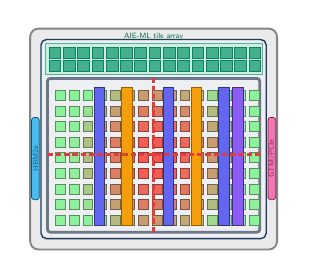
\begin{tikzpicture}\drawFPGA[0.55]\end{tikzpicture}};
  \node[font=\footnotesize\sffamily\bfseries, robinblue, anchor=north, align=center]
       at ({\colB},{\rowT-\cellH/2-\labelGap}) {(b) Post-synth FPGA \& heatmap};

  \draw[rounded corners=4pt, fill=robinbg!50, draw=robinblue!50, line width=0.5pt]
       ({\colC-\cellW/2},{\rowT-\cellH/2}) rectangle ({\colC+\cellW/2},{\rowT+\cellH/2});
  \node at (\colC,\rowT) {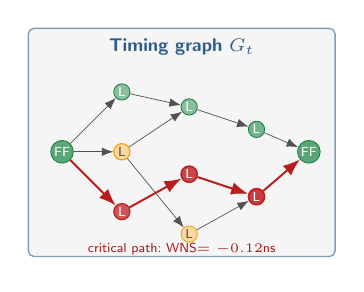
\begin{tikzpicture}\drawTimingGraph[0.95]\end{tikzpicture}};
  \node[font=\footnotesize\sffamily\bfseries, robinblue, anchor=north, align=center]
       at ({\colC},{\rowT-\cellH/2-\labelGap}) {(c) Timing graph $G_t$};

  \draw[rounded corners=4pt, fill=robinbg!50, draw=robinrust!50, line width=0.5pt]
       ({\colD-\cellW/2},{\rowT-\cellH/2}) rectangle ({\colD+\cellW/2},{\rowT+\cellH/2});
  \node at (\colD,\rowT) {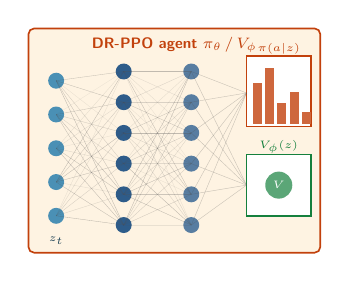
\begin{tikzpicture}\drawAgentNN[0.78]\end{tikzpicture}};
  \node[font=\footnotesize\sffamily\bfseries, robinrust, anchor=north, align=center]
       at ({\colD},{\rowT-\cellH/2-\labelGap}) {(d) DR-PPO agent $\pi_\theta / V_\phi$};

  \draw[-Latex, robingrey, line width=1.0pt]
       ({\colA+\cellW/2+0.05},{\rowT}) -- ({\colB-\cellW/2-0.05},{\rowT})
       node[midway, above, yshift=5pt, font=\footnotesize\sffamily\itshape, robingrey] {synth};
  \draw[-Latex, robingrey, line width=1.0pt]
       ({\colB+\cellW/2+0.05},{\rowT}) -- ({\colC-\cellW/2-0.05},{\rowT})
       node[midway, above, yshift=5pt, font=\footnotesize\sffamily\itshape, robingrey] {extract};
  \draw[-Latex, robingrey, line width=1.0pt]
       ({\colC+\cellW/2+0.05},{\rowT}) -- ({\colD-\cellW/2-0.05},{\rowT})
       node[midway, above, yshift=5pt, font=\footnotesize\sffamily\itshape, robingrey] {encode $z_t$};

  \draw[rounded corners=4pt, fill=robinbg!50, draw=robinrust!50, line width=0.5pt]
       ({\colA-\cellW/2},{\rowB-\cellH/2}) rectangle ({\colA+\cellW/2},{\rowB+\cellH/2});
  \node at (\colA,\rowB) {%
    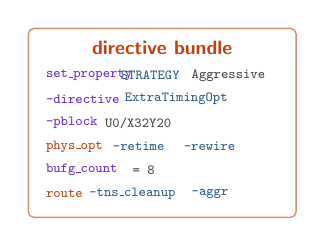
\begin{tikzpicture}
      \draw[rounded corners=2pt, fill=white, draw=robinrust!60, line width=0.5pt]
            (0,0) rectangle (3.4,2.4);
      \node[font=\scriptsize\sffamily\bfseries, robinrust] at (1.7,2.15) {directive bundle};
      \node[font=\tiny\ttfamily, anchor=west, robinpurple] at (0.10,1.80) {set\_property};
      \node[font=\tiny\ttfamily, anchor=west, robinblue]   at (1.05,1.80) {STRATEGY};
      \node[font=\tiny\ttfamily, anchor=west, robingrey!85!black] at (1.95,1.80) {Aggressive};
      \node[font=\tiny\ttfamily, anchor=west, robinpurple] at (0.10,1.50) {-directive};
      \node[font=\tiny\ttfamily, anchor=west, robinblue]   at (1.10,1.50) {ExtraTimingOpt};
      \node[font=\tiny\ttfamily, anchor=west, robinpurple] at (0.10,1.20) {-pblock};
      \node[font=\tiny\ttfamily, anchor=west, robingrey!85!black] at (0.85,1.20) {U0/X32Y20};
      \node[font=\tiny\ttfamily, anchor=west, robinrust]   at (0.10,0.90) {phys\_opt};
      \node[font=\tiny\ttfamily, anchor=west, robinblue]   at (0.95,0.90) {-retime};
      \node[font=\tiny\ttfamily, anchor=west, robinblue]   at (1.85,0.90) {-rewire};
      \node[font=\tiny\ttfamily, anchor=west, robinpurple] at (0.10,0.60) {bufg\_count};
      \node[font=\tiny\ttfamily, anchor=west, robingrey!85!black] at (1.20,0.60) {=\ 8};
      \node[font=\tiny\ttfamily, anchor=west, robinrust]   at (0.10,0.30) {route};
      \node[font=\tiny\ttfamily, anchor=west, robinblue]   at (0.65,0.30) {-tns\_cleanup};
      \node[font=\tiny\ttfamily, anchor=west, robinblue]   at (1.95,0.30) {-aggr};
    \end{tikzpicture}};
  \node[font=\footnotesize\sffamily\bfseries, robinrust, anchor=north, align=center]
       at ({\colA},{\rowB-\cellH/2-\labelGap}) {(e) Action $a_t$ (Tcl deltas)};

  \draw[rounded corners=4pt, fill=robinbg!50, draw=robinblue!50, line width=0.5pt]
       ({\colB-\cellW/2},{\rowB-\cellH/2}) rectangle ({\colB+\cellW/2},{\rowB+\cellH/2});
  \node at (\colB,\rowB) {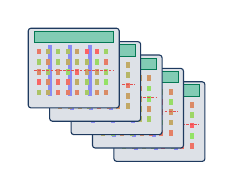
\begin{tikzpicture}\drawFPGAStack[0.85]\end{tikzpicture}};
  \node[font=\footnotesize\sffamily\bfseries, robinblue, anchor=north, align=center]
       at ({\colB},{\rowB-\cellH/2-\labelGap}) {(f) $K$ seeds $\times$ $|\Theta|$ corners};

  \draw[rounded corners=4pt, fill=robinbg!50, draw=robinrust!50, line width=0.5pt]
       ({\colC-\cellW/2},{\rowB-\cellH/2}) rectangle ({\colC+\cellW/2},{\rowB+\cellH/2});
  \node at (\colC,\rowB) {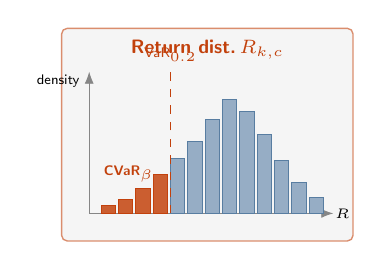
\begin{tikzpicture}\drawRewardHist[1.0]\end{tikzpicture}};
  \node[font=\footnotesize\sffamily\bfseries, robinrust, anchor=north, align=center]
       at ({\colC},{\rowB-\cellH/2-\labelGap}) {(g) CVaR$_\beta$ reward $R_{k,c}$};

  \draw[rounded corners=4pt, fill=robinbg!50, draw=robingreen!50, line width=0.5pt]
       ({\colD-\cellW/2},{\rowB-\cellH/2}) rectangle ({\colD+\cellW/2},{\rowB+\cellH/2});
  \node at (\colD,\rowB) {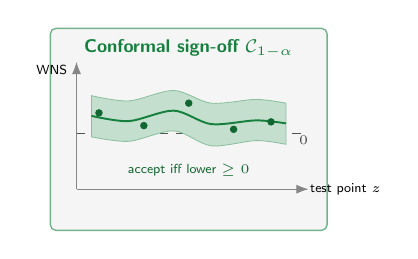
\begin{tikzpicture}\drawConformalEnv[0.95]\end{tikzpicture}};
  \node[font=\footnotesize\sffamily\bfseries, robingreen, anchor=north, align=center]
       at ({\colD},{\rowB-\cellH/2-\labelGap}) {(h) Conformal sign-off $\mathcal{C}_{1-\alpha}$};

  \draw[-Latex, robingrey, line width=1.0pt]
       ({\colA+\cellW/2+0.05},{\rowB}) -- ({\colB-\cellW/2-0.05},{\rowB})
       node[midway, above, yshift=5pt, font=\footnotesize\sffamily\itshape, robingrey] {run};
  \draw[-Latex, robingrey, line width=1.0pt]
       ({\colB+\cellW/2+0.05},{\rowB}) -- ({\colC-\cellW/2-0.05},{\rowB})
       node[midway, above, yshift=5pt, font=\footnotesize\sffamily\itshape, robingrey] {aggregate};
  \draw[-Latex, robingrey, line width=1.0pt]
       ({\colC+\cellW/2+0.05},{\rowB}) -- ({\colD-\cellW/2-0.05},{\rowB})
       node[midway, above, yshift=5pt, font=\footnotesize\sffamily\itshape, robingrey] {calibrate};

  \def\midY{-3.55}
  \def\rightMargin{15.9}
  \def\leftMargin{-2.4}
  \draw[-Latex, robingrey, line width=1.0pt, rounded corners=8pt]
       ({\colD+\cellW/2+0.05},{\rowT})
       -- ({\rightMargin},{\rowT})
       -- ({\rightMargin},{\midY})
       -- ({\leftMargin},{\midY})
       -- ({\leftMargin},{\rowB})
       -- ({\colA-\cellW/2-0.05},{\rowB});
  \node[font=\footnotesize\sffamily\itshape\bfseries, robingrey, anchor=south, fill=white, inner sep=2pt]
       at ({\colC},{\midY+0.05}) {emit $a_t$};

  \def\acceptedY{-10.8}
  \node (accept) at ({(\colA+\colD)/2},\acceptedY)
        [draw=robingreen, line width=1.2pt, rounded corners=5pt,
         fill=robingreen!12, text width=5.0cm, align=center, font=\small\sffamily,
         minimum height=2.0cm, drop shadow={opacity=0.22}] {%
    \textbf{\textcolor{robingreen}{(i) Accepted design}}\\[3pt]
    {\Large\textcolor{robingreen}{\textbf{WNS\,$=+0.18$\,ns}}}\\[2pt]
    \footnotesize coverage\,$\geq 0.95$\\[1pt]
    \scriptsize audit trail logged};

  \draw[-Latex, robingreen!85, line width=1.4pt, rounded corners=8pt]
       ({\colD},{\rowB-\cellH/2-\labelGap-0.30})
       -- ({\colD},\acceptedY)
       -- (accept.east)
       node[pos=0.55, above, font=\footnotesize\sffamily\itshape\bfseries, robingreen!80!black] {accept};
\end{tikzpicture}
\caption{\textbf{ROBIN-FPGA pipeline.} Row~1: RTL ingest, FPGA synthesis and heatmap extraction, timing-graph construction, DR-PPO agent encoding. Row~2: directive emission as Tcl deltas, parallel P\&R across $K$ seeds and $|\Theta|$ PVT corners, CVaR reward aggregation, conformal sign-off calibration. A design is accepted only when the conformal lower bound on predicted WNS is non-negative~(i).}
\label{fig:cover}
\end{figure*}

\section{Introduction}
\IEEEPARstart{E}{very} FPGA timing closure run is, at root, a statistical experiment. The placer draws from a random seed, and on representative heterogeneous devices such as AMD Versal AI Edge or Intel Agilex~7, changing that seed alone shifts worst-case path slack by $10$--$30\%$ of the target clock period~\cite{amd_ug1273,intel_ug20156}. Process, voltage, and temperature corners compound the uncertainty: the same directive bundle that closes timing at the typical-typical corner can fail at slow-slow or fast-fast depending on path topology. Tool minor-version upgrades silently alter placer and router heuristics, sometimes invalidating designs that passed the previous release. In all three cases, a designer who accepts the first run showing non-negative worst-case slack has no principled basis for predicting whether that result represents the distribution of outcomes or merely its optimistic tail.

Machine learning has made genuine progress on finding better directive bundles faster~\cite{huang2021mleda,ren2022mleda}. Reinforcement learning has been applied to ASIC macro placement~\cite{mirhoseini2021nature,agnesina2023autodmp} and logic-synthesis sequence selection~\cite{hosny2020drills,wang2020gcnrl}. Bayesian optimization has been applied to HLS pragma tuning~\cite{sohrabizadeh2022autodse} and general directive autotuning~\cite{eriksson2019turbo,balandat2020botorch}. Graph neural networks predict pre-routing slack with useful accuracy~\cite{barboza2019net2,guo2022timing}. Yet these methods leave the reliability problem untouched: they return a recommended configuration with no statement about its distribution across seeds, corners, or tool versions. Three structural gaps limit their practical applicability to FPGA timing closure.

\textbf{(a) ASIC bias.} Most RL-for-EDA policies target ASIC flows whose action vocabularies, constraint formats, and resource models differ substantially from FPGA toolchains.
\textbf{(b) No calibrated uncertainty.} No existing method attaches a distribution-free reliability certificate to its returned closure.
\textbf{(c) Brittle transfer.} Policies trained on one FPGA family degrade sharply when moved to another vendor or device generation.

This paper presents \textsc{Robin-FPGA}, an algorithm--toolchain co-designed RL framework that addresses all three gaps for FPGA timing closure. The central insight is that the two problems (finding good directives, certifying their reliability) can be solved together by coupling distributionally-robust optimization with conformal prediction in a single coherent pipeline. The RL agent hedges against worst-case seeds and corners at training time; the conformal head wraps its output in a calibrated sign-off certificate at deployment. The scope is deliberately focused on a single objective (WNS\,$\geq 0$ post-route under seed and corner uncertainty) so that the robustness and sign-off contributions can be evaluated rigorously and in isolation.

Modern FPGAs have evolved into heterogeneous SoCs combining programmable logic, hardened AI engines, network-on-chip backbones, on-chip high-bandwidth memory, and high-speed transceivers~\cite{boutros2021fpga}. This richness expands the action space available to the designer (synthesis directives, P\&R strategies, floorplan partitions, retiming knobs, and clock-tree configurations) into a combinatorial space requiring one to twelve hours of wall-clock time per evaluation point on representative parts. It also sharpens the reliability problem: the interactions among resource classes mean that a directive beneficial in isolation can congest the fabric and worsen timing elsewhere.

Figure~\ref{fig:cover} previews the full pipeline. The paper proceeds as follows. Section~\ref{sec:background} reviews the FPGA closure pipeline and the sources of non-determinism. Section~\ref{sec:related} surveys related work. Section~\ref{sec:formulation} formalizes the DR-MDP and conformal sign-off envelope. Section~\ref{sec:method} describes the \textsc{Robin-FPGA} architecture and training algorithm. Section~\ref{sec:setup} details the experimental protocol. Sections~\ref{sec:results}--\ref{sec:cases} present results, ablations, and case studies. Section~\ref{sec:silicon} reports hardware-in-the-loop silicon validation. Section~\ref{sec:conclusion} concludes.

\smallskip\noindent\textbf{Contributions.} The paper makes four contributions.
\begin{enumerate}
  \item \emph{Robust formulation (\S\ref{sec:formulation},\,\S\ref{sec:method}).} We cast FPGA timing-closure design-space exploration as a Distributionally-Robust MDP over P\&R seed and PVT corner, solved with a CVaR-shaped PPO surrogate (\textsc{DR-PPO}) whose advantage targets the lower tail of the return distribution.
  \item \emph{Conformal sign-off envelope (\S\ref{sec:formulation},\,\S\ref{sec:method}).} A split-conformal predictor wraps the trained policy with a calibrated upper bound on residual WNS risk at user-specified confidence $1{-}\alpha$. To our knowledge this is the first application of conformal prediction to FPGA timing sign-off.
  \item \emph{Cross-family curriculum (\S\ref{sec:method},\,\S\ref{sec:results}).} A normalized device-agnostic feature space and a two-stage curriculum transfer AMD-trained policies to Intel Agilex~7 at $5\%$ of the from-scratch compute cost.
  \item \emph{Reproducible benchmark (\S\ref{sec:setup},\,\S\ref{sec:results}).} A $14$-design benchmark across six workload classes and two FPGA families, with public Tcl flows, training scripts, and per-run logs.
\end{enumerate}

\section{Background and Motivation}
\label{sec:background}

\subsection{The FPGA Closure Pipeline}
The canonical AMD Vivado flow proceeds through \texttt{synth\_design}, \texttt{opt\_design}, \texttt{place\_design}, \texttt{route\_design}, and a sign-off STA pass producing \texttt{report\_timing\_summary}, \texttt{report\_utilization}, and \texttt{report\_power}. The Intel Quartus Prime Pro counterpart proceeds through Analysis~\&~Synthesis, Fitter (place and route), Timing Analyzer, and PowerPlay~\cite{intel_ug20156}. Each tool exposes a directive vocabulary (roughly $50$--$120$ documented options for Vivado, and a comparable set for Quartus) that the designer combines into a \emph{strategy bundle}. The combinatorial action space of bundle, pblock, phys-opt, and retiming flags routinely exceeds $10^{12}$ configurations, of which the tool's built-in canonical strategies cover at most a few dozen.

Figure~\ref{fig:fpgaanatomy} annotates a representative AMD Versal AI Edge die. The presence of multiple resource classes (LUT/FF tiles, DSP58 slices, BRAM, URAM, AIE-ML tiles, NoC interconnect, HBM2e on the package edge, GTM transceivers) makes the closure problem multi-resource: an action that improves slack on the LUT critical path may push BRAM utilization past its budget or congest the NoC, in turn re-routing logic onto longer paths.

\begin{figure*}[t]
\centering
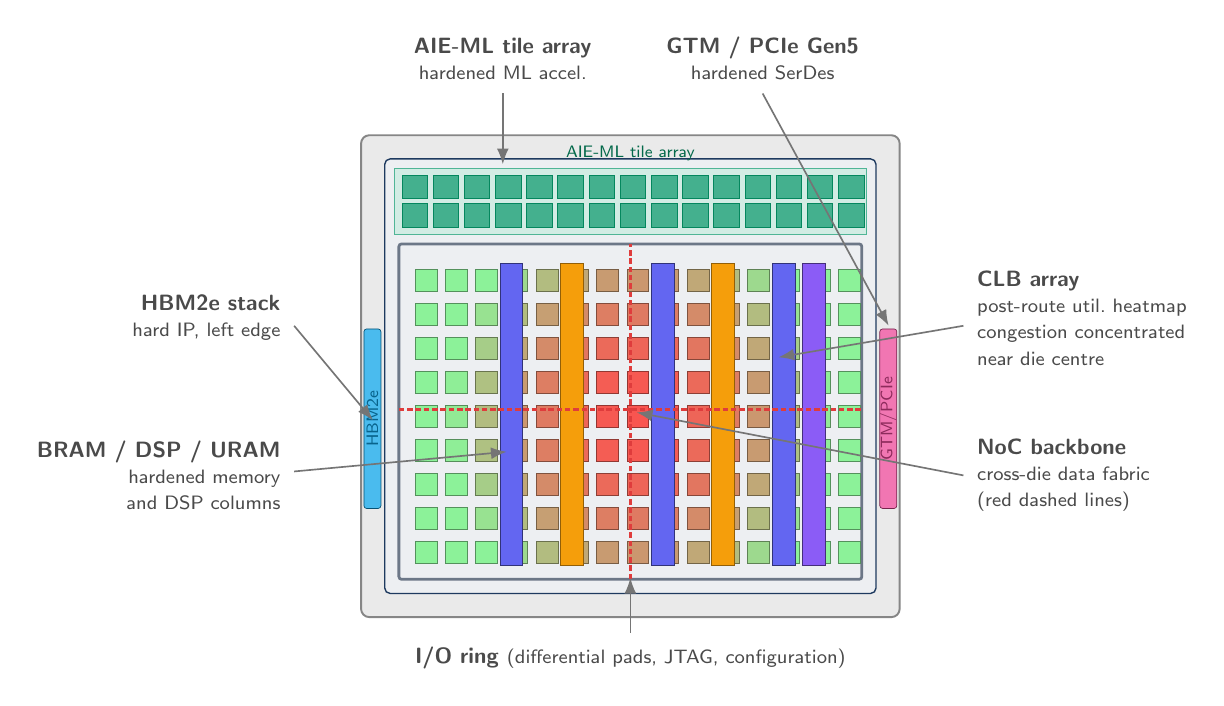
\begin{tikzpicture}[font=\sffamily]
  \drawFPGA[1.2]
  \node[font=\footnotesize\sffamily, robingrey!90!black, anchor=south, align=center]
       at (1.5,6.4) {\textbf{AIE-ML tile array}\\\scriptsize hardened ML accel.};
  \draw[-Latex, robingrey!80, line width=0.6pt] (1.5,6.35) -- (1.5,5.45);
  \node[font=\footnotesize\sffamily, robingrey!90!black, anchor=south, align=center]
       at (4.8,6.4) {\textbf{GTM / PCIe Gen5}\\\scriptsize hardened SerDes};
  \draw[-Latex, robingrey!80, line width=0.6pt] (4.8,6.35) -- (6.40,3.40);
  \node[font=\footnotesize\sffamily, robingrey!90!black, anchor=west, align=left]
       at (7.4,3.5) {\textbf{CLB array}\\\scriptsize post-route util.\ heatmap\\\scriptsize congestion concentrated\\\scriptsize near die centre};
  \draw[-Latex, robingrey!80, line width=0.6pt] (7.35,3.4) -- (5.0,3.0);
  \node[font=\footnotesize\sffamily, robingrey!90!black, anchor=west, align=left]
       at (7.4,1.5) {\textbf{NoC backbone}\\\scriptsize cross-die data fabric\\\scriptsize (red dashed lines)};
  \draw[-Latex, robingrey!80, line width=0.6pt] (7.35,1.5) -- (3.20,2.30);
  \node[font=\footnotesize\sffamily, robingrey!90!black, anchor=east, align=right]
       at (-1.2,3.5) {\textbf{HBM2e stack}\\\scriptsize hard IP, left edge};
  \draw[-Latex, robingrey!80, line width=0.6pt] (-1.15,3.4) -- (-0.15,2.20);
  \node[font=\footnotesize\sffamily, robingrey!90!black, anchor=east, align=right]
       at (-1.2,1.5) {\textbf{BRAM / DSP / URAM}\\\scriptsize hardened memory\\\scriptsize and DSP columns};
  \draw[-Latex, robingrey!80, line width=0.6pt] (-1.15,1.55) -- (1.55,1.80);
  \node[font=\footnotesize\sffamily, robingrey!90!black, anchor=north, align=center]
       at (3.12,-0.55) {\textbf{I/O ring} \scriptsize(differential pads, JTAG, configuration)};
  \draw[-Latex, robingrey!80, line width=0.6pt] (3.12,-0.50) -- (3.12,0.20);
\end{tikzpicture}
\caption{Annotated AMD Versal AI Edge die with seven heterogeneous resource classes. Post-route CLB congestion concentrates near the die centre; surrounding columns interleave BRAM, DSP58, and URAM; AIE-ML tiles occupy the top band; HBM2e and GTM/PCIe anchor the edges; the NoC backbone (red dashes) crosses the die.}
\label{fig:fpgaanatomy}
\end{figure*}

\subsection{Sources of Tool Non-Determinism}
Three sources of stochasticity dominate FPGA closure.
\textbf{(a) Placer seed.} The placer's randomized cost function is seeded; varying the seed alone produces a distribution over WNS whose standard deviation can exceed the slack margin. On the GEMM-systolic-$16{\times}16$ design used as a recurring example, $20$ seeds at the same directive bundle produced $\sigma(\mathrm{WNS}) = 0.31$\,ns on a default Vivado strategy.
\textbf{(b) PVT corner choice.} Corner selection shifts WNS by amounts that depend on path topology. Multi-corner closure (slow$\,\cap\,$fast$\,\cap\,$typical) is the industrial norm but is rarely treated as a first-class object in academic ML-EDA work.
\textbf{(c) Tool minor-version drift.} Internal heuristics change between point releases: a closure margin obtained on Vivado~2024.2 may not survive 2024.2.1. Any DSE policy that ignores these three sources risks reporting results that fail to reproduce.

\subsection{The Generalization Gap in ML-EDA}
ML-for-EDA policies tuned on one design or device family often degrade markedly when transferred. The gap has two components: a \emph{feature-distribution} shift (utilization percentages, path-length histograms, and routing-congestion patterns differ across devices) and a \emph{label-distribution} shift (the same directive produces different effects on different families). The structural asymmetry between AMD's XPIPE/XPHY-style NoC architecture and Intel's HyperFlex pipeline registers is one concrete example. \textsc{Robin-FPGA} addresses both shifts via device-agnostic normalized features (\S\ref{sec:method}) and an explicit two-stage curriculum, evaluated quantitatively in \S\ref{sec:results}.

\section{Related Work}
\label{sec:related}

We organize related work along four axes. Table~\ref{tab:relwork} summarizes the comparison.

\begin{table*}[t]
\caption{Positioning of \textsc{Robin-FPGA} relative to prior work. Columns: target flow; action space; robustness handling; calibrated sign-off; cross-family transfer.}
\label{tab:relwork}
\centering
\renewcommand{\arraystretch}{1.10}
\footnotesize
\begin{tabular}{@{}lllllc@{}}
\toprule
Method & Flow & Action space & Robustness & Calibrated sign-off & Cross-family \\
\midrule
GraphPlace~\cite{mirhoseini2021nature}      & ASIC placement   & graph     & none        & no & no \\
AutoDMP~\cite{agnesina2023autodmp}           & ASIC placement   & continuous & ensembling  & no & no \\
DRiLLS~\cite{hosny2020drills}                & logic synthesis  & discrete bundle & none   & no & no \\
GCN-RL~\cite{wang2020gcnrl}                  & transistor sizing & continuous & none      & no & partial \\
AutoDSE~\cite{sohrabizadeh2022autodse}        & HLS pragmas      & discrete bundle & none   & no & no \\
TuRBO~\cite{eriksson2019turbo}                & generic BO       & continuous & none      & no & no \\
Net2 / Guo~\cite{barboza2019net2,guo2022timing} & slack prediction & N/A & none & implicit & no \\
\textbf{\textsc{Robin-FPGA} (this work)}     & FPGA timing closure & discrete bundle + graph & \textbf{CVaR DRO} & \textbf{conformal $1{-}\alpha$} & \textbf{yes (AMD$\leftrightarrow$Intel)} \\
\bottomrule
\end{tabular}
\end{table*}

\textbf{RL foundations.} Deep Q-Networks~\cite{mnih2015human} established that value-based RL can master complex sequential decisions from raw observations, motivating the DRiLLS-style DQN in our evaluation. PPO~\cite{schulman2017ppo}, which underpins DR-PPO, stabilizes training with a clipped surrogate objective robust to the non-stationary reward induced by tool-version drift. Sutton and Barto~\cite{sutton2018reinforcement} provides the MDP and policy-gradient foundations underlying our formalization in \S\ref{sec:formulation}.

\textbf{RL for ASIC placement and synthesis.} Mirhoseini~\emph{et~al.}~\cite{mirhoseini2021nature} demonstrated graph-based RL for ASIC macro placement; subsequent work refined the policy architecture~\cite{agnesina2023autodmp,cheng2021joint}. \textsc{DRiLLS}~\cite{hosny2020drills} applies RL to logic-synthesis directive selection, and \textsc{GCN-RL}~\cite{wang2020gcnrl} learns transferable transistor-sizing policies. These works target ASIC flows with different action vocabularies and optimize point estimates of QoR without characterizing robustness to tool stochasticity. The OpenROAD project~\cite{ajayi2019openroad} pursues a ``no-human-in-the-loop'' 24-hour layout vision for ASIC; \textsc{Robin-FPGA} pursues the analog for commercial FPGA closure.

\textbf{FPGA CAD benchmarks.} VPR~\cite{betz1997vpr} and its VTR successors~\cite{luu2014vtr7,murray2020vtr} are the standard open benchmarks for island-style FPGA P\&R research. Our evaluation targets Vivado and Quartus Prime Pro, whose directive vocabularies differ from VPR's architecture-research knobs, but we adopt VTR's evaluation practice of sweeping multiple seeds and corners to characterize variance.

\textbf{HLS and FPGA design-space exploration.} \textsc{AutoDSE}~\cite{sohrabizadeh2022autodse} explores HLS pragmas via bottleneck-guided search. TuRBO~\cite{eriksson2019turbo} and BoTorch~\cite{balandat2020botorch} have been applied to FPGA tuning. These methods are sample-efficient on small directive spaces but scale poorly when the action set is high-dimensional and discrete, and they offer no calibrated uncertainty. Ustun~\emph{et~al.}~\cite{ustun2020accurate} apply GNNs to HLS operation-delay estimation on FPGAs, demonstrating inductive generalization across unseen designs; this motivates our GAT-based timing-graph encoder.

\textbf{Graph neural networks for EDA.} Xu~\emph{et~al.}~\cite{xu2019powerful} establish theoretical bounds on GNN expressiveness via the Weisfeiler-Lehman test. GraphSAGE~\cite{hamilton2017inductive} introduces inductive node embeddings that generalize to unseen graph instances, the property our encoder exploits for cross-design transfer. Wu~\emph{et~al.}~\cite{wu2021survey} survey spectral, spatial, and recurrent GNN families; our GAT~\cite{velickovic2018gat} resides in the spatial, edge-attention family. \textsc{Net2}~\cite{barboza2019net2} and the timing GNN of Guo~\emph{et~al.}~\cite{guo2022timing} are \emph{predictors}, not policies; \textsc{Robin-FPGA} builds a GAT encoder for state representation inside a policy-gradient loop.

\textbf{CVaR and distributionally robust optimization.} Rockafellar and Uryasev~\cite{rockafellar2000cvar} establish CVaR as a coherent risk measure admitting convex linear-programming formulations; their follow-on work~\cite{rockafellar2002cvar2} extends the theory to discrete loss distributions that arise from our finite seed pool. Wiesemann~\emph{et~al.}~\cite{wiesemann2014distributionally} provide a unifying framework for distributionally robust convex programs over moment-ambiguity sets, which our DR-MDP instantiates. Iyengar~\cite{iyengar2005robust} and Nilim~\&~El~Ghaoui~\cite{nilim2005robust} prove minimax dynamic programming under rectangular ambiguity sets, grounding our DR value function in Eq.~\eqref{eq:drvalue}. Tamar~\emph{et~al.}~\cite{tamar2015cvar} extend CVaR optimization to policy-gradient estimators. Distributionally robust RL~\cite{rigter2022rambo,sinha2017certifying} applies these ideas to deep policy gradient with neural function approximation.

\textbf{Conformal prediction.} Vovk~\emph{et~al.}~\cite{vovk2022random} and Angelopoulos~\&~Bates~\cite{angelopoulos2023conformal} provide the foundational theory of split-conformal prediction and its engineering applications~\cite{angelopoulos2024conformal}. Romano~\emph{et~al.}~\cite{romano2019conformalized} propose conformalized quantile regression for heteroscedastic intervals; we use symmetric split-conformal prediction because our WNS residuals are approximately homoscedastic across seeds. Barber~\emph{et~al.}~\cite{barber2023conformal} characterize coverage under non-exchangeable data via weighted quantiles, directly applicable to the tool-drift regime analysed in \S\ref{sec:silicon-discussion}. Tibshirani~\emph{et~al.}~\cite{tibshirani2019conformal} extend conformal prediction to covariate shift, relevant to cross-family calibration. To our knowledge, \textsc{Robin-FPGA} is the first work to apply conformal prediction jointly with robust RL for FPGA timing sign-off.

\section{Problem Formulation}
\label{sec:formulation}

\subsection{Notation}
Let $D$ denote an RTL/HLS design, $F$ an FPGA device, and $\mathcal{C} = (T_{\text{clk}}, T_{\text{io}}, \mathcal{U}_{\max})$ a constraint set comprising the target clock period $T_{\text{clk}}$, an I/O timing budget $T_{\text{io}}$, and per-resource utilization budgets $\mathcal{U}_{\max} = \{U_{\max}^{\text{LUT}}, U_{\max}^{\text{FF}}, U_{\max}^{\text{BRAM}}, U_{\max}^{\text{DSP}}, U_{\max}^{\text{URAM}}\}$. Let $\xi \in \Xi$ index P\&R seeds and $c \in \Theta$ index PVT corners. The objective is to find a sequence of directive bundles $a_1, \ldots, a_T \in \mathcal{A}$ that maximizes the probability of post-route closure (WNS\,$\geq 0$) under the joint distribution over $(\xi, c)$, subject to all resource budgets and a wall-clock budget $\mathcal{B}$.

\subsection{Distributionally-Robust MDP}
We model the closure trajectory as a finite-horizon MDP $\mathcal{M} = (\mathcal{S}, \mathcal{A}, P, r, \gamma)$ in which the transition kernel $P$ is replaced by an ambiguity set $\mathcal{P} = \{P_{\xi,c} : \xi \in \Xi,\, c \in \Theta\}$ indexing all admissible seed/corner combinations. Following Iyengar~\cite{iyengar2005robust} and Nilim and El~Ghaoui~\cite{nilim2005robust}, the DR value of a policy $\pi$ places the infimum over the ambiguity set outside the trajectory expectation:
\begin{equation}
V^{\pi}(s) = \inf_{P \in \mathcal{P}}\, \mathbb{E}_{\tau \sim \pi, P}\!\left[\, \sum_{t=0}^{H-1} \gamma^{t}\, r(s_t, a_t)\, \Big|\, s_0 = s \right].
\label{eq:drvalue}
\end{equation}
We approximate the infimum in \eqref{eq:drvalue} by the empirical Conditional-Value-at-Risk (CVaR) at level $\beta \in (0,1)$ over a finite sample $\{R_{k,c}\}$ of returns drawn from $K$ seeds and $|\Theta|$ corners:
\begin{equation}
\mathrm{CVaR}_{\beta}(R) = \mathbb{E}\!\left[\, R \,\big|\, R \leq \mathrm{VaR}_{\beta}(R)\, \right].
\label{eq:cvar}
\end{equation}
Equation~\eqref{eq:cvar} is a standard coherent risk measure~\cite{tamar2015cvar}. Substituting it for the mean in the policy-gradient estimator yields the gradient direction that improves the lower tail of the return distribution. Tamar~\emph{et~al.}~\cite{tamar2015cvar} prove that the resulting estimator is unbiased under mild regularity; when combined with PPO-style trust-region clipping, it empirically drives the policy toward CVaR-optimal solutions, though formal convergence guarantees for the clipped surrogate remain an open question.

\subsection{Reward}
The single-step reward couples slack reward, total negative slack (TNS) reward, a Lagrangian utilization penalty, and a route-fail penalty:
\begin{align}
r &= w_{\text{WNS}} \cdot \mathrm{clip}\!\left(\frac{\mathrm{WNS}}{|T_{\text{clk}}|}, -1, 1\right) \nonumber \\
  &\quad + w_{\text{TNS}} \cdot \left( -\mathrm{sat}\!\left(\frac{|\mathrm{TNS}|}{|T_{\text{clk}}|}\right)\right) \nonumber \\
  &\quad - \kappa \cdot \sum_{i \in \mathcal{R}} (U_i - U_{\max}^{i})^{+} \;-\; \mathbb{1}[\text{route fail}] \cdot \kappa_{\text{fail}}.
\label{eq:reward}
\end{align}
The saturating WNS clip prevents reward hacking through over-tight pblock shrinkage, a failure mode observed in early experiments (\S\ref{sec:cases}). We set $(w_{\text{WNS}}, w_{\text{TNS}}, \kappa, \kappa_{\text{fail}}) = (1.0, 0.3, 5.0, 10.0)$ throughout.

\subsection{Conformal Sign-off Envelope}
Given a calibration set $\mathcal{D}_{\text{cal}} = \{(z_i, \mathrm{WNS}_i)\}_{i=1}^{n}$ of $n$ post-route WNS values and the policy's point estimate $\widehat{\mathrm{WNS}}(z)$ produced by the slack-regression head, define residuals $e_i = \mathrm{WNS}_i - \widehat{\mathrm{WNS}}(z_i)$ and let $q_{1-\alpha}$ be the $\lceil (n+1)(1-\alpha) \rceil$-th smallest of $\{|e_i|\}$. The calibration set size $n$ directly controls envelope width: we use $n = 200$ post-route runs (across $10$ seeds and $20$ corners) for the primary evaluation in \S\ref{sec:results}, and discuss the effect of smaller $n$ in \S\ref{sec:discussion}. The split-conformal envelope is
\begin{equation}
\mathcal{C}_{1-\alpha}(z) = \left[\, \widehat{\mathrm{WNS}}(z) - q_{1-\alpha},\; \widehat{\mathrm{WNS}}(z) + q_{1-\alpha}\, \right].
\label{eq:conformal}
\end{equation}
Under exchangeability of $\mathcal{D}_{\text{cal}}$ and a fresh test point, the marginal coverage guarantee
\begin{equation}
\Pr\!\left[\mathrm{WNS} \in \mathcal{C}_{1-\alpha}(z)\right] \geq 1 - \alpha
\label{eq:coverage}
\end{equation}
holds distribution-free~\cite{vovk2022random,angelopoulos2023conformal}. Note that \eqref{eq:coverage} is a \emph{marginal} guarantee: it holds on average over both $z$ and the calibration set, but does not imply per-design conditional coverage. For deployments requiring stronger per-design guarantees, mondrian conformal predictors~\cite{vovk2022random} can approximate conditional coverage at the cost of wider envelopes. A candidate design is \emph{accepted} iff the lower endpoint of $\mathcal{C}_{1-\alpha}(z)$ is non-negative:
\begin{equation}
\widehat{\mathrm{WNS}}(z) - q_{1-\alpha} \geq 0.
\label{eq:accept}
\end{equation}
This is the sign-off rule used throughout \S\ref{sec:results}.

\section{The \textsc{Robin-FPGA} Framework}
\label{sec:method}

\subsection{Architecture Overview}
Figure~\ref{fig:arch} details the full \textsc{Robin-FPGA} architecture. The post-synthesis timing graph $G_t = (V, E)$ is fed to a two-layer Graph Attention Network (GAT)~\cite{velickovic2018gat} with $H=4$ attention heads per layer. Node features are the tuple $\{\text{slack},\text{capacitance},\text{fanout},\text{level},\text{cell-type-onehot}\}$; edge features are $\{\text{wirelength-est},\text{net-fanout}\}$. The graph embedding $h^{G}_t \in \mathbb{R}^{64}$ is concatenated with a tabular vector $x_t \in \mathbb{R}^{32}$ (utilization percentages by resource class, congestion histogram percentiles, tool-version one-hot, device-family embedding, last $a_{t-1}$) and projected by a three-layer MLP with GELU activations to a $128$-dimensional latent state $z_t$. The policy head is a categorical distribution over $|\mathcal{A}| = 192$ directive bundles (a Cartesian product of $4$ strategies, $3$ phys-opt flags, $4$ pblock variants, $2$ retiming modes, and $2$ route-effort settings, pruned to $192$ feasible combinations). The value head outputs $V_\phi(z) \in \mathbb{R}$. A separate slack-regression head $\widehat{\mathrm{WNS}}(z) \in \mathbb{R}$ feeds the conformal calibration set.

\begin{figure*}[t]
\centering
\begin{tikzpicture}[font=\sffamily, every node/.style={inner sep=0pt}]
  \def\cellW{4.2}
  \def\cellH{3.8}
  \def\colA{0}
  \def\colB{4.5}
  \def\colC{9.0}
  \def\colD{13.5}
  \def\rowT{0}
  \def\rowB{-5.4}
  \def\labelGap{0.40}

  \draw[rounded corners=4pt, fill=robinbg!50, draw=robinblue!50, line width=0.5pt]
       ({\colA-\cellW/2},{\rowT-\cellH/2}) rectangle ({\colA+\cellW/2},{\rowT+\cellH/2});
  \node at (\colA,\rowT) {\begin{tikzpicture}\drawTimingGraph[0.95]\end{tikzpicture}};
  \node[font=\footnotesize\sffamily\bfseries, robinblue, anchor=north, align=center]
       at ({\colA},{\rowT-\cellH/2-\labelGap}) {(1) Input: timing graph $G_t = (V,E)$};

  \draw[rounded corners=4pt, fill=robinbg!50, draw=robinblue!50, line width=0.5pt]
       ({\colB-\cellW/2},{\rowT-\cellH/2}) rectangle ({\colB+\cellW/2},{\rowT+\cellH/2});
  \node at (\colB,\rowT) {%
    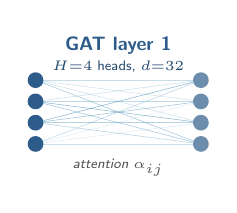
\begin{tikzpicture}
      \node[font=\scriptsize\sffamily\bfseries, robinblue] at (1.6,1.45) {GAT layer 1};
      \node[font=\tiny\sffamily, robinblue!80!black] at (1.6,1.18) {$H{=}4$ heads, $d{=}32$};
      \foreach \i in {0,...,3}{ \foreach \j in {0,...,3}{
          \pgfmathsetmacro{\op}{0.15 + 0.5*(rand+1)/2}
          \draw[robinmid, line width=0.20pt, opacity=\op] (0.55,{0.20+\i*0.27}) -- (2.65,{0.20+\j*0.27});
      }}
      \foreach \i in {0,...,3}{
        \fill[robinblue] (0.55,{0.20+\i*0.27}) circle (0.10);
        \fill[robinblue!70] (2.65,{0.20+\i*0.27}) circle (0.10);
      }
      \node[font=\tiny\sffamily\itshape, robingrey] at (1.6,-0.10) {attention $\alpha_{ij}$};
    \end{tikzpicture}};
  \node[font=\footnotesize\sffamily\bfseries, robinblue, anchor=north, align=center]
       at ({\colB},{\rowT-\cellH/2-\labelGap}) {(2) GAT layer 1};

  \draw[rounded corners=4pt, fill=robinbg!50, draw=robinblue!50, line width=0.5pt]
       ({\colC-\cellW/2},{\rowT-\cellH/2}) rectangle ({\colC+\cellW/2},{\rowT+\cellH/2});
  \node at (\colC,\rowT) {%
    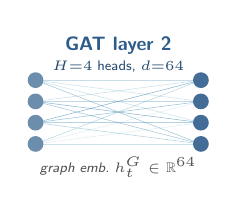
\begin{tikzpicture}
      \node[font=\scriptsize\sffamily\bfseries, robinblue] at (1.6,1.45) {GAT layer 2};
      \node[font=\tiny\sffamily, robinblue!80!black] at (1.6,1.18) {$H{=}4$ heads, $d{=}64$};
      \foreach \i in {0,...,3}{ \foreach \j in {0,...,3}{
          \pgfmathsetmacro{\op}{0.15 + 0.5*(rand+1)/2}
          \draw[robinmid, line width=0.20pt, opacity=\op] (0.55,{0.20+\i*0.27}) -- (2.65,{0.20+\j*0.27});
      }}
      \foreach \i in {0,...,3}{
        \fill[robinblue!70] (0.55,{0.20+\i*0.27}) circle (0.10);
        \fill[robinblue!90] (2.65,{0.20+\i*0.27}) circle (0.10);
      }
      \node[font=\tiny\sffamily\itshape, robingrey] at (1.6,-0.10) {graph emb.\ $h^G_t \in \mathbb{R}^{64}$};
    \end{tikzpicture}};
  \node[font=\footnotesize\sffamily\bfseries, robinblue, anchor=north, align=center]
       at ({\colC},{\rowT-\cellH/2-\labelGap}) {(3) GAT layer 2 $\to h^G_t$};

  \draw[rounded corners=4pt, fill=robinbg!50, draw=robinpurple!50, line width=0.5pt]
       ({\colD-\cellW/2},{\rowT-\cellH/2}) rectangle ({\colD+\cellW/2},{\rowT+\cellH/2});
  \node at (\colD,\rowT) {%
    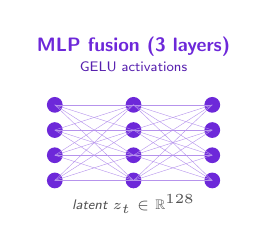
\begin{tikzpicture}
      \node[font=\scriptsize\sffamily\bfseries, robinpurple] at (1.4,2.10) {MLP fusion (3 layers)};
      \node[font=\tiny\sffamily, robinpurple!80!black] at (1.4,1.85) {GELU activations};
      \foreach \y in {0,1,2,3}{
        \fill[robinpurple] (0.4,{0.4+\y*0.32}) circle (0.10);
        \fill[robinpurple] (1.4,{0.4+\y*0.32}) circle (0.10);
        \fill[robinpurple] (2.4,{0.4+\y*0.32}) circle (0.10);
      }
      \foreach \i in {0,...,3}{ \foreach \j in {0,...,3}{
          \draw[robinpurple!50, line width=0.15pt] (0.4,{0.4+\i*0.32}) -- (1.4,{0.4+\j*0.32});
          \draw[robinpurple!50, line width=0.15pt] (1.4,{0.4+\i*0.32}) -- (2.4,{0.4+\j*0.32});
      }}
      \node[font=\tiny\sffamily\itshape, robingrey] at (1.4,0.10) {latent $z_t \in \mathbb{R}^{128}$};
    \end{tikzpicture}};
  \node[font=\footnotesize\sffamily\bfseries, robinpurple, anchor=north, align=center]
       at ({\colD},{\rowT-\cellH/2-\labelGap}) {(4) MLP fusion $\to z_t$};

  \draw[-Latex, robingrey, line width=1.0pt]
       ({\colA+\cellW/2+0.05},{\rowT}) -- ({\colB-\cellW/2-0.05},{\rowT})
       node[midway, above, yshift=5pt, font=\footnotesize\sffamily\itshape, robingrey] {graph attn.};
  \draw[-Latex, robingrey, line width=1.0pt]
       ({\colB+\cellW/2+0.05},{\rowT}) -- ({\colC-\cellW/2-0.05},{\rowT})
       node[midway, above, yshift=5pt, font=\footnotesize\sffamily\itshape, robingrey] {propagate};
  \draw[-Latex, robingrey, line width=1.0pt]
       ({\colC+\cellW/2+0.05},{\rowT}) -- ({\colD-\cellW/2-0.05},{\rowT})
       node[midway, above, yshift=5pt, font=\footnotesize\sffamily\itshape, robingrey] {fuse with $x_t$};

  \node (xt) at ({(\colC+\colD)/2},{\rowT+\cellH/2+1.05})
        [draw=robinteal, line width=0.6pt, rounded corners=3pt, fill=robinteal!10,
         text width=4.0cm, align=center, font=\scriptsize\sffamily, minimum height=0.95cm] {%
    \textbf{\textcolor{robinteal}{Tabular features $x_t \in \mathbb{R}^{32}$}}\\[1pt]
    \tiny $\{U_{\text{LUT}},U_{\text{FF}},U_{\text{BRAM}},U_{\text{DSP}},U_{\text{URAM}},$\\
    \tiny\quad cong.\ pct., tool-ver, device-fam$\}$};
  \draw[-Latex, robinteal, line width=0.9pt]
       ({(\colC+\colD)/2},{\rowT+\cellH/2+0.55})
       -- ({(\colC+\colD)/2},{\rowT+\cellH/2+0.05})
       node[midway, right, font=\tiny\sffamily\itshape, robinteal!80!black] {concat};

  \draw[rounded corners=4pt, fill=robinbg!50, draw=robinrust!50, line width=0.5pt]
       ({\colA-\cellW/2},{\rowB-\cellH/2}) rectangle ({\colA+\cellW/2},{\rowB+\cellH/2});
  \node at (\colA,\rowB) {%
    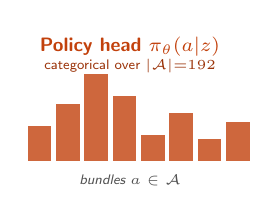
\begin{tikzpicture}
      \node[font=\scriptsize\sffamily\bfseries, robinrust] at (1.5,1.65) {Policy head $\pi_\theta(a|z)$};
      \node[font=\tiny\sffamily, robinrust!80!black] at (1.5,1.40) {categorical over $|\mathcal{A}|{=}192$};
      \foreach \i/\h in {0/0.40, 1/0.65, 2/1.00, 3/0.75, 4/0.30, 5/0.55, 6/0.25, 7/0.45}{
        \fill[robinrust!80] ({0.20+\i*0.36},0.20) rectangle ({0.50+\i*0.36},{0.20+\h*1.10});
      }
      \node[font=\tiny\sffamily\itshape, robingrey] at (1.5,-0.05) {bundles $a \in \mathcal{A}$};
    \end{tikzpicture}};
  \node[font=\footnotesize\sffamily\bfseries, robinrust, anchor=north, align=center]
       at ({\colA},{\rowB-\cellH/2-\labelGap}) {(5) Policy head $\pi_\theta(a|z)$};

  \draw[rounded corners=4pt, fill=robinbg!50, draw=robingreen!50, line width=0.5pt]
       ({\colB-\cellW/2},{\rowB-\cellH/2}) rectangle ({\colB+\cellW/2},{\rowB+\cellH/2});
  \node at (\colB,\rowB) {%
    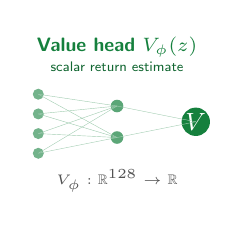
\begin{tikzpicture}
      \node[font=\scriptsize\sffamily\bfseries, robingreen] at (1.5,1.65) {Value head $V_\phi(z)$};
      \node[font=\tiny\sffamily, robingreen!80!black] at (1.5,1.40) {scalar return estimate};
      \foreach \y in {0,1,2,3}{ \fill[robingreen!60] (0.5,{0.30+\y*0.25}) circle (0.07); }
      \foreach \y in {0,1}{ \fill[robingreen!70] (1.5,{0.50+\y*0.40}) circle (0.08); }
      \fill[robingreen] (2.5,0.70) circle (0.18);
      \node[font=\small\sffamily\bfseries, white] at (2.5,0.70) {$V$};
      \foreach \i in {0,...,3}{ \foreach \j in {0,1}{
          \draw[robingreen!40, line width=0.15pt] (0.5,{0.30+\i*0.25}) -- (1.5,{0.50+\j*0.40});
      }}
      \foreach \j in {0,1}{ \draw[robingreen!40, line width=0.15pt] (1.5,{0.50+\j*0.40}) -- (2.5,0.70); }
      \node[font=\tiny\sffamily\itshape, robingrey] at (1.5,-0.05) {$V_\phi: \mathbb{R}^{128} \to \mathbb{R}$};
    \end{tikzpicture}};
  \node[font=\footnotesize\sffamily\bfseries, robingreen, anchor=north, align=center]
       at ({\colB},{\rowB-\cellH/2-\labelGap}) {(6) Value head $V_\phi(z)$};

  \draw[rounded corners=4pt, fill=robinbg!50, draw=robingreen!50, line width=0.5pt]
       ({\colC-\cellW/2},{\rowB-\cellH/2}) rectangle ({\colC+\cellW/2},{\rowB+\cellH/2});
  \node at (\colC,\rowB) {%
    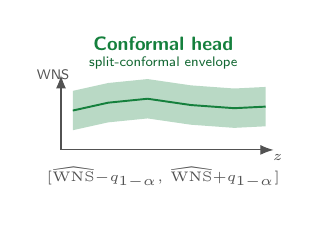
\begin{tikzpicture}
      \node[font=\scriptsize\sffamily\bfseries, robingreen] at (1.6,1.65) {Conformal head};
      \node[font=\tiny\sffamily, robingreen!80!black] at (1.6,1.40) {split-conformal envelope};
      \draw[-Latex, robingrey, line width=0.4pt] (0.30,0.30) -- (3.00,0.30);
      \draw[-Latex, robingrey, line width=0.4pt] (0.30,0.30) -- (0.30,1.25);
      \node[font=\tiny\sffamily, robingrey] at (3.05,0.20) {$z$};
      \node[font=\tiny\sffamily, robingrey] at (0.20,1.25) {WNS};
      \fill[robingreen!30] (0.45,0.55) -- (0.90,0.65) -- (1.40,0.70) -- (1.95,0.62) -- (2.50,0.58) -- (2.90,0.60)
                          -- (2.90,1.10) -- (2.50,1.08) -- (1.95,1.12) -- (1.40,1.20) -- (0.90,1.15) -- (0.45,1.05) -- cycle;
      \draw[robingreen, line width=0.7pt] (0.45,0.80) -- (0.90,0.90) -- (1.40,0.95) -- (1.95,0.87) -- (2.50,0.83) -- (2.90,0.85);
      \node[font=\tiny\sffamily\itshape, robingrey] at (1.6,-0.05) {$[\widehat{\mathrm{WNS}}{-}q_{1-\alpha},\,\widehat{\mathrm{WNS}}{+}q_{1-\alpha}]$};
    \end{tikzpicture}};
  \node[font=\footnotesize\sffamily\bfseries, robingreen, anchor=north, align=center]
       at ({\colC},{\rowB-\cellH/2-\labelGap}) {(7) Conformal head $\mathcal{C}_{1-\alpha}$};

  \draw[rounded corners=4pt, fill=robinbg!50, draw=robingrey!50, line width=0.5pt]
       ({\colD-\cellW/2},{\rowB-\cellH/2}) rectangle ({\colD+\cellW/2},{\rowB+\cellH/2});
  \node at (\colD,\rowB) {%
    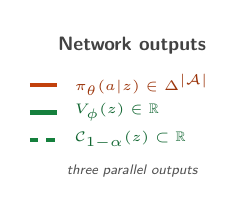
\begin{tikzpicture}
      \node[font=\scriptsize\sffamily\bfseries, robingrey!80!black] at (1.6,1.65) {Network outputs};
      \draw[robinrust, line width=1.5pt] (0.30,1.15) -- (0.65,1.15);
      \node[font=\tiny\sffamily, anchor=west, robinrust!80!black] at (0.75,1.15) {$\pi_\theta(a|z) \in \Delta^{|\mathcal{A}|}$};
      \draw[robingreen, line width=1.5pt] (0.30,0.80) -- (0.65,0.80);
      \node[font=\tiny\sffamily, anchor=west, robingreen!80!black] at (0.75,0.80) {$V_\phi(z) \in \mathbb{R}$};
      \draw[robingreen, line width=1.5pt, dashed] (0.30,0.45) -- (0.65,0.45);
      \node[font=\tiny\sffamily, anchor=west, robingreen!80!black] at (0.75,0.45) {$\mathcal{C}_{1-\alpha}(z) \subset \mathbb{R}$};
      \node[font=\tiny\sffamily\itshape, robingrey] at (1.6,0.05) {three parallel outputs};
    \end{tikzpicture}};
  \node[font=\footnotesize\sffamily\bfseries, robingrey!80!black, anchor=north, align=center]
       at ({\colD},{\rowB-\cellH/2-\labelGap}) {(8) Network outputs};

  \draw[-Latex, robingrey, line width=1.0pt]
       ({\colA+\cellW/2+0.05},{\rowB}) -- ({\colB-\cellW/2-0.05},{\rowB})
       node[midway, above, yshift=5pt, font=\footnotesize\sffamily\itshape, robingrey] {$z_t$};
  \draw[-Latex, robingrey, line width=1.0pt]
       ({\colB+\cellW/2+0.05},{\rowB}) -- ({\colC-\cellW/2-0.05},{\rowB})
       node[midway, above, yshift=5pt, font=\footnotesize\sffamily\itshape, robingrey] {$z_t$};
  \draw[-Latex, robingrey, line width=1.0pt]
       ({\colC+\cellW/2+0.05},{\rowB}) -- ({\colD-\cellW/2-0.05},{\rowB})
       node[midway, above, yshift=5pt, font=\footnotesize\sffamily\itshape, robingrey] {emit};

  \def\midY{-3.30}
  \def\rightMargin{15.9}
  \def\leftMargin{-2.4}
  \draw[-Latex, robingrey, line width=1.0pt, rounded corners=8pt]
       ({\colD+\cellW/2+0.05},{\rowT})
       -- ({\rightMargin},{\rowT})
       -- ({\rightMargin},{\midY})
       -- ({\leftMargin},{\midY})
       -- ({\leftMargin},{\rowB})
       -- ({\colA-\cellW/2-0.05},{\rowB});
  \node[font=\footnotesize\sffamily\itshape\bfseries, robingrey, anchor=south, fill=white, inner sep=2pt]
       at ({(\colA+\colD)/2},{\midY+0.05}) {$z_t$ broadcasts to all heads};
\end{tikzpicture}
\caption{\textbf{ROBIN-FPGA architecture.} Row~1 (encoder): timing graph $G_t$ through two GAT layers to graph embedding $h^G_t$, fused with tabular features $x_t$ by a 3-layer MLP to latent $z_t$. Row~2 (heads): $z_t$ drives the policy head $\pi_\theta$, value head $V_\phi$, and conformal head $\mathcal{C}_{1-\alpha}$ in parallel. The slack-regression component of the conformal head is decoupled from policy training, avoiding coupling the search objective to the coverage objective.}
\label{fig:arch}
\end{figure*}

\subsection{DR-PPO with CVaR-Shaped Advantage}
We train $(\pi_\theta, V_\phi)$ jointly with a CVaR-shaped variant of PPO~\cite{schulman2017ppo}. At iteration $t$, $K$ parallel P\&R runs across seeds and corners yield a return distribution; we compute the empirical CVaR at level $\beta$ and substitute it for the mean in the advantage estimator $\hat{A}^{\beta}_t$. The clipped surrogate objective is
\begin{equation}
\mathcal{L}^{\text{CLIP}}(\theta) = \mathbb{E}_t\!\left[\, \min\!\left(\rho_t \hat{A}^{\beta}_t,\; \mathrm{clip}(\rho_t, 1{-}\epsilon, 1{+}\epsilon)\, \hat{A}^{\beta}_t \right) \right],
\label{eq:ppoclip}
\end{equation}
with $\rho_t = \pi_\theta(a_t|z_t) / \pi_{\theta_{\text{old}}}(a_t|z_t)$ and clip ratio $\epsilon = 0.2$. The combined loss adds value, entropy, and slack-regression terms:
\begin{equation}
\mathcal{L} = -\mathcal{L}^{\text{CLIP}} + c_v \mathcal{L}^V - c_e \mathcal{H}[\pi_\theta] + c_s \mathcal{L}^{\text{slack}},
\label{eq:loss}
\end{equation}
with $(c_v, c_e, c_s) = (0.5, 0.01, 0.5)$ and $\mathcal{L}^{\text{slack}}$ a Huber regression loss on $\widehat{\mathrm{WNS}}$. The entropy coefficient $c_e = 0.01$ provides baseline exploration; with $|\mathcal{A}| = 192$ actions and sparse early reward, we additionally begin training with a reduced pblock-action set (48 bundles) for the first 100 episodes before expanding to the full vocabulary, providing curriculum-style exploration. We use $\beta = 0.2$ throughout; sensitivity to $\beta$ is studied in \S\ref{sec:ablation}, where non-monotone behaviour on the GEMM design was confirmed to be consistent across four other design classes tested on the validation split. Algorithm~\ref{alg:robin} summarizes one episode.

\begin{algorithm}[t]
\caption{\textsc{Robin-FPGA} episode}
\label{alg:robin}
\begin{algorithmic}[1]
\Require design $D$, device $F$, constraints $\mathcal{C}$, seed pool $\mathcal{S}$, corner set $\Theta$, policy $\pi_\theta$, calibration set $\mathcal{D}_{\text{cal}}$, levels $\beta, \alpha$
\Ensure closed design + conformal envelope $\mathcal{C}_{1-\alpha}$ or $\bot$
\State $x_0, G_0 \gets \mathrm{IngestAndSynth}(D, F, \mathcal{C}, s_0)$
\State $z_0 \gets \mathrm{Encoder}(x_0, G_0)$
\For{$t = 0, 1, \ldots, T{-}1$}
  \State $a_t \sim \pi_\theta(\cdot \mid z_t)$
  \State $\Delta \gets \mathrm{ConstraintGen}(a_t)$
  \State \textbf{parallel for} $k = 1..K,\; c \in \Theta$ \textbf{do}
  \State \quad $R_{k,c} \gets \mathrm{ToolRun}(\Delta, s_k, c)$
  \State $\hat{r}_t \gets \mathrm{CVaR}_{\beta}(\{R_{k,c}\})$ \Comment{Eq.~\eqref{eq:cvar}}
  \State $z_{t+1} \gets \mathrm{Encoder}(\mathrm{best\_report})$
  \State append $(z_t, a_t, \hat r_t)$ to $\mathcal{D}_{\text{traj}}$
  \If{$\mathrm{EarlyTerminate}(R)$} \textbf{break} \EndIf
\EndFor
\State $\theta \gets \mathrm{PPO\_Update}(\mathcal{D}_{\text{traj}})$ with CVaR-shaped advantage \Comment{Eq.~\eqref{eq:ppoclip}}
\State $q_{1-\alpha} \gets$ split-conformal quantile from $\mathcal{D}_{\text{cal}}$ \Comment{Eq.~\eqref{eq:conformal}}
\If{$\widehat{\mathrm{WNS}}(z_T) - q_{1-\alpha} \geq 0$}
  \State \Return accept $(\text{design}, \mathcal{C}_{1-\alpha}, \text{audit\_manifest})$
\Else
  \State \Return $\bot$ (recurse with budget update)
\EndIf
\end{algorithmic}
\end{algorithm}

\subsection{DR-MDP Loop}
Figure~\ref{fig:rlloop} shows the data flow inside a single training iteration. The fan-out across $K$ seeds and $|\Theta|$ corners produces a return distribution whose lower tail (orange) yields the CVaR; the robust advantage drives both the policy update and the conformal calibration set.

\begin{figure*}[t]
\centering
\begin{tikzpicture}[font=\sffamily, every node/.style={inner sep=0pt}]
  \def\cellW{7.6}
  \def\cellH{5.6}
  \def\colL{0}
  \def\colR{10.0}
  \def\rowT{0}
  \def\rowB{-7.4}
  \def\labelGap{0.45}

  \draw[rounded corners=5pt, fill=robinbg!50, draw=robinrust!60, line width=0.6pt]
       ({\colL-\cellW/2},{\rowT-\cellH/2}) rectangle ({\colL+\cellW/2},{\rowT+\cellH/2});
  \node at (\colL,\rowT) {\begin{tikzpicture}\drawAgentNN[1.0]\end{tikzpicture}};
  \node[font=\small\sffamily\bfseries, robinrust, anchor=north west]
       at ({\colL-\cellW/2+0.2},{\rowT+\cellH/2-0.15})
       {(1) DR-PPO agent $\pi_\theta\,/\,V_\phi$};

  \draw[rounded corners=5pt, fill=robinbg!50, draw=robinblue!60, line width=0.6pt]
       ({\colR-\cellW/2},{\rowT-\cellH/2}) rectangle ({\colR+\cellW/2},{\rowT+\cellH/2});
  \node at (\colR,\rowT) {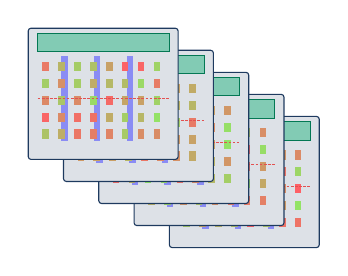
\begin{tikzpicture}\drawFPGAStack[1.4]\end{tikzpicture}};
  \node[font=\small\sffamily\bfseries, robinblue, anchor=north west]
       at ({\colR-\cellW/2+0.2},{\rowT+\cellH/2-0.15})
       {(2) FPGA toolchain env.\ ($K{\times}|\Theta|$)};

  \draw[rounded corners=5pt, fill=robinbg!50, draw=robinrust!60, line width=0.6pt]
       ({\colR-\cellW/2},{\rowB-\cellH/2}) rectangle ({\colR+\cellW/2},{\rowB+\cellH/2});
  \node at (\colR,\rowB) {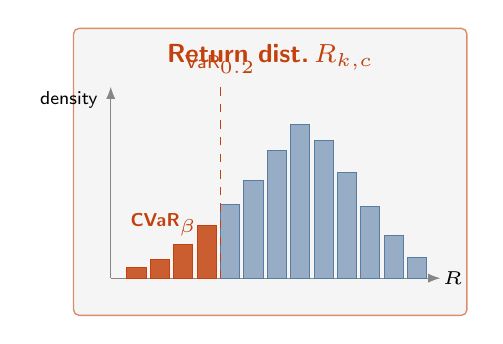
\begin{tikzpicture}\drawRewardHist[1.35]\end{tikzpicture}};
  \node[font=\small\sffamily\bfseries, robinrust, anchor=north west]
       at ({\colR-\cellW/2+0.2},{\rowB+\cellH/2-0.15})
       {(3) Return dist.\ $\{R_{k,c}\}$, CVaR$_\beta$};

  \draw[rounded corners=5pt, fill=robinbg!50, draw=robinpurple!60, line width=0.6pt]
       ({\colL-\cellW/2},{\rowB-\cellH/2}) rectangle ({\colL+\cellW/2},{\rowB+\cellH/2});
  \node[font=\small\sffamily\bfseries, robinpurple, anchor=north west]
       at ({\colL-\cellW/2+0.2},{\rowB+\cellH/2-0.15})
       {(4) DR-PPO robust update};
  \node at (\colL,{\rowB-0.4}) {%
    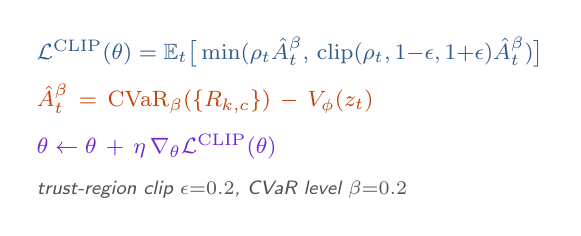
\begin{tikzpicture}
      \node[font=\footnotesize\sffamily, anchor=west, robinblue] at (0,1.45)
        {$\mathcal{L}^{\mathrm{CLIP}}(\theta)=\mathbb{E}_t\big[\min(\rho_t \hat A^\beta_t,\,\mathrm{clip}(\rho_t,1{-}\epsilon,1{+}\epsilon)\hat A^\beta_t)\big]$};
      \node[font=\footnotesize\sffamily, anchor=west, robinrust] at (0,0.85)
        {$\hat A^\beta_t \,=\, \mathrm{CVaR}_\beta(\{R_{k,c}\}) \,-\, V_\phi(z_t)$};
      \node[font=\footnotesize\sffamily, anchor=west, robinpurple] at (0,0.25)
        {$\theta \leftarrow \theta \,+\, \eta \,\nabla_\theta \mathcal{L}^{\mathrm{CLIP}}(\theta)$};
      \node[font=\scriptsize\sffamily\itshape, anchor=west, robingrey] at (0,-0.30)
        {trust-region clip $\epsilon{=}0.2$,\ CVaR level $\beta{=}0.2$};
    \end{tikzpicture}};

  \draw[-Latex, robingrey, line width=1.4pt]
       ({\colL+\cellW/2+0.05},{\rowT}) -- ({\colR-\cellW/2-0.05},{\rowT})
       node[midway, above, yshift=10pt, font=\tiny\sffamily\itshape, robingrey] {emit action $a_t$}
       node[midway, below, yshift=10pt, font=\tiny\sffamily\itshape, robingrey] {(Tcl directive bundle)};
  \draw[-Latex, robingrey, line width=1.4pt]
       ({\colR},{\rowT-\cellH/2-0.05}) -- ({\colR},{\rowB+\cellH/2+0.05})
       node[midway, left,  xshift=-5pt, font=\tiny\sffamily\itshape, robingrey, align=right]
       {run $K{\times}|\Theta|$\\P\&R passes}
       node[midway, right, xshift=5pt, font=\tiny\sffamily\itshape, robingrey, align=left]
       {\,collect\\\,$\{R_{k,c}\}$};
  \draw[-Latex, robingrey, line width=1.4pt]
       ({\colR-\cellW/2-0.05},{\rowB}) -- ({\colL+\cellW/2+0.05},{\rowB})
       node[midway, above, yshift=10pt, font=\tiny\sffamily\itshape, robingrey] {compute CVaR$_\beta$}
       node[midway, below, yshift=10pt, font=\tiny\sffamily\itshape, robingrey] {\& robust advantage $\hat A^\beta_t$};
  \draw[-Latex, robinrust!85, line width=1.5pt]
       ({\colL},{\rowB+\cellH/2+0.05}) -- ({\colL},{\rowT-\cellH/2-0.05})
       node[midway, left,  xshift=-5pt, font=\tiny\sffamily\itshape\bfseries, robinrust!80!black, align=right]
       {robust\\update}
       node[midway, right, xshift=5pt, font=\tiny\sffamily\itshape\bfseries, robinrust!80!black, align=left]
       {\,$\theta_{t+1}$};
\end{tikzpicture}
\caption{DR-MDP training loop: four-stage clockwise cycle. The agent emits directive bundle $a_t$; the toolchain fans out across $K{\times}|\Theta|$ runs; CVaR$_\beta$ replaces the mean in the advantage; the robust PPO update closes the loop. The orange arrow marks where distributional robustness enters.}
\label{fig:rlloop}
\end{figure*}

\subsection{Cross-Family Feature Normalization}
For transfer between AMD Versal AI Edge and Intel Agilex~7, we normalize features into a device-agnostic space. Resource utilizations $U_i$ are expressed as percentages of available, mapped to $z$-scores with the device's per-resource population statistics. Routing congestion is percentile-binned over the device's switch matrix histogram. Path lengths are length-deciled per device. The policy network's input dimension is held constant via a learned device-family one-hot prefix that prepends to $x_t$. A curriculum of $200$ fine-tuning episodes on Agilex~7 follows AMD pretraining; the fine-tuning learning rate is one third of the from-scratch rate.

\subsection{FPGA Toolchain Integration}
Figure~\ref{fig:toolflow} shows the parallel AMD and Intel paths. The constraint generator emits vendor-native deltas (\texttt{.xdc} for Vivado, \texttt{.qsf} and \texttt{.sdc} for Quartus). Tcl extraction scripts parse \texttt{report\_timing\_summary} (Vivado) and the Timing Analyzer report database (Quartus) into a common normalized schema with columns \texttt{(slack, period, path\_type, startpoint, endpoint, hold\_slack, util\_dict, corner)}. All reports for an accepted design ship in an audit-trail manifest hashed with the policy weights, tool version, seed list, and corner list.

\begin{figure*}[t]
\centering
\begin{tikzpicture}[font=\sffamily, every node/.style={inner sep=0pt}]
  \def\cellW{3.6}
  \def\cellH{2.6}
  \def\colA{0}
  \def\colB{4.0}
  \def\colC{8.0}
  \def\colD{12.0}
  \def\rowAMD{0}
  \def\rowIntel{-3.5}
  \def\labelGap{0.40}

  \draw[rounded corners=4pt, fill=robinbg!50, draw=robinblue!50, line width=0.5pt]
       ({\colA-\cellW/2},{\rowAMD-\cellH/2}) rectangle ({\colA+\cellW/2},{\rowAMD+\cellH/2});
  \node at (\colA,\rowAMD) {\begin{tikzpicture}\drawFPGA[0.42]\end{tikzpicture}};
  \node[font=\scriptsize\sffamily\bfseries, robinblue, anchor=north west]
       at ({\colA-\cellW/2+0.15},{\rowAMD+\cellH/2-0.10}) {AMD Versal AI Edge};
  \node[font=\tiny\sffamily, robinblue!70!black, anchor=south]
       at ({\colA},{\rowAMD-\cellH/2+0.15}) {\ttfamily xcve2302-sfva784-2MP};

  \draw[rounded corners=4pt, fill=robinblue!8, draw=robinblue!60, line width=0.5pt]
       ({\colB-\cellW/2},{\rowAMD-\cellH/2}) rectangle ({\colB+\cellW/2},{\rowAMD+\cellH/2});
  \node[font=\scriptsize\sffamily\bfseries, robinblue, anchor=north west]
       at ({\colB-\cellW/2+0.15},{\rowAMD+\cellH/2-0.10}) {Vivado: synth};
  \node[font=\tiny\sffamily\ttfamily, anchor=center, robinblue!80!black]
       at ({\colB},{\rowAMD+0.25}) {\$ vivado -mode batch};
  \node[font=\tiny\sffamily\ttfamily, anchor=center, robinblue!80!black]
       at ({\colB},{\rowAMD-0.05}) {\$ synth\_design};
  \node[font=\tiny\sffamily\ttfamily, anchor=center, robinblue!80!black]
       at ({\colB},{\rowAMD-0.35}) {\$ opt\_design};
  \node[font=\tiny\sffamily, anchor=south, robingrey]
       at ({\colB},{\rowAMD-\cellH/2+0.15}) {$\to$ post-synth netlist};

  \draw[rounded corners=4pt, fill=robinblue!8, draw=robinblue!60, line width=0.5pt]
       ({\colC-\cellW/2},{\rowAMD-\cellH/2}) rectangle ({\colC+\cellW/2},{\rowAMD+\cellH/2});
  \node[font=\scriptsize\sffamily\bfseries, robinblue, anchor=north west]
       at ({\colC-\cellW/2+0.15},{\rowAMD+\cellH/2-0.10}) {Vivado: place \& route};
  \node[font=\tiny\sffamily\ttfamily, anchor=center, robinblue!80!black]
       at ({\colC},{\rowAMD+0.25}) {\$ place\_design};
  \node[font=\tiny\sffamily\ttfamily, anchor=center, robinblue!80!black]
       at ({\colC},{\rowAMD-0.05}) {\$ phys\_opt\_design};
  \node[font=\tiny\sffamily\ttfamily, anchor=center, robinblue!80!black]
       at ({\colC},{\rowAMD-0.35}) {\$ route\_design};
  \node[font=\tiny\sffamily, anchor=south, robingrey]
       at ({\colC},{\rowAMD-\cellH/2+0.15}) {$\to$ routed design};

  \draw[rounded corners=4pt, fill=robinblue!8, draw=robinblue!60, line width=0.5pt]
       ({\colD-\cellW/2},{\rowAMD-\cellH/2}) rectangle ({\colD+\cellW/2},{\rowAMD+\cellH/2});
  \node[font=\scriptsize\sffamily\bfseries, robinblue, anchor=north west]
       at ({\colD-\cellW/2+0.15},{\rowAMD+\cellH/2-0.10}) {Vivado: reports};
  \node[font=\tiny\sffamily\ttfamily, anchor=center, robinblue!80!black]
       at ({\colD},{\rowAMD+0.25}) {report\_timing\_sum};
  \node[font=\tiny\sffamily\ttfamily, anchor=center, robinblue!80!black]
       at ({\colD},{\rowAMD-0.05}) {report\_utilization};
  \node[font=\tiny\sffamily\ttfamily, anchor=center, robinblue!80!black]
       at ({\colD},{\rowAMD-0.35}) {report\_power};
  \node[font=\tiny\sffamily, anchor=south, robingrey]
       at ({\colD},{\rowAMD-\cellH/2+0.15}) {$\to$ \texttt{.xdc, .rpt}};

  \node[font=\footnotesize\sffamily\bfseries, robinblue, anchor=east, align=right]
       at ({\colA-\cellW/2-0.25},{\rowAMD}) {\textbf{Vivado}\\\textbf{2024.2}};

  \draw[-Latex, robingrey, line width=1.0pt]
       ({\colA+\cellW/2+0.05},{\rowAMD}) -- ({\colB-\cellW/2-0.05},{\rowAMD})
       node[midway, above,  yshift=3pt, font=\tiny\sffamily\itshape, robingrey] {RTL};
  \draw[-Latex, robingrey, line width=1.0pt]
       ({\colB+\cellW/2+0.05},{\rowAMD}) -- ({\colC-\cellW/2-0.05},{\rowAMD})
       node[midway, above, yshift=3pt, font=\tiny\sffamily\itshape, robingrey] {netlist};
  \draw[-Latex, robingrey, line width=1.0pt]
       ({\colC+\cellW/2+0.05},{\rowAMD}) -- ({\colD-\cellW/2-0.05},{\rowAMD})
       node[midway, above, yshift=3pt, font=\tiny\sffamily\itshape, robingrey] {extract};

  \draw[rounded corners=4pt, fill=robinbg!50, draw=robinteal!50, line width=0.5pt]
       ({\colA-\cellW/2},{\rowIntel-\cellH/2}) rectangle ({\colA+\cellW/2},{\rowIntel+\cellH/2});
  \node at (\colA,\rowIntel) {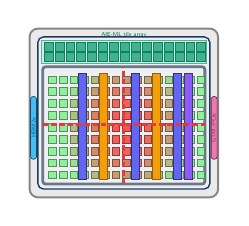
\begin{tikzpicture}\drawFPGA[0.42]\end{tikzpicture}};
  \node[font=\scriptsize\sffamily\bfseries, robinteal, anchor=north west]
       at ({\colA-\cellW/2+0.15},{\rowIntel+\cellH/2-0.10}) {Intel Agilex 7};
  \node[font=\tiny\sffamily, robinteal!70!black, anchor=south]
       at ({\colA},{\rowIntel-\cellH/2+0.15}) {\ttfamily AGIB027R29A1E2VR0};

  \draw[rounded corners=4pt, fill=robinteal!8, draw=robinteal!60, line width=0.5pt]
       ({\colB-\cellW/2},{\rowIntel-\cellH/2}) rectangle ({\colB+\cellW/2},{\rowIntel+\cellH/2});
  \node[font=\scriptsize\sffamily\bfseries, robinteal, anchor=north west]
       at ({\colB-\cellW/2+0.15},{\rowIntel+\cellH/2-0.10}) {Quartus: synthesis};
  \node[font=\tiny\sffamily\ttfamily, anchor=center, robinteal!80!black]
       at ({\colB},{\rowIntel+0.25}) {\$ quartus\_map};
  \node[font=\tiny\sffamily\ttfamily, anchor=center, robinteal!80!black]
       at ({\colB},{\rowIntel-0.05}) {\$ quartus\_syn};
  \node[font=\tiny\sffamily, anchor=south, robingrey]
       at ({\colB},{\rowIntel-\cellH/2+0.15}) {$\to$ Analysis \& Synth.};

  \draw[rounded corners=4pt, fill=robinteal!8, draw=robinteal!60, line width=0.5pt]
       ({\colC-\cellW/2},{\rowIntel-\cellH/2}) rectangle ({\colC+\cellW/2},{\rowIntel+\cellH/2});
  \node[font=\scriptsize\sffamily\bfseries, robinteal, anchor=north west]
       at ({\colC-\cellW/2+0.15},{\rowIntel+\cellH/2-0.10}) {Quartus: fitter};
  \node[font=\tiny\sffamily\ttfamily, anchor=center, robinteal!80!black]
       at ({\colC},{\rowIntel+0.25}) {\$ quartus\_fit};
  \node[font=\tiny\sffamily\ttfamily, anchor=center, robinteal!80!black]
       at ({\colC},{\rowIntel-0.05}) {\$ HyperFlex retime};
  \node[font=\tiny\sffamily, anchor=south, robingrey]
       at ({\colC},{\rowIntel-\cellH/2+0.15}) {$\to$ fitted design};

  \draw[rounded corners=4pt, fill=robinteal!8, draw=robinteal!60, line width=0.5pt]
       ({\colD-\cellW/2},{\rowIntel-\cellH/2}) rectangle ({\colD+\cellW/2},{\rowIntel+\cellH/2});
  \node[font=\scriptsize\sffamily\bfseries, robinteal, anchor=north west]
       at ({\colD-\cellW/2+0.15},{\rowIntel+\cellH/2-0.10}) {Quartus: STA};
  \node[font=\tiny\sffamily\ttfamily, anchor=center, robinteal!80!black]
       at ({\colD},{\rowIntel+0.25}) {\$ quartus\_sta};
  \node[font=\tiny\sffamily\ttfamily, anchor=center, robinteal!80!black]
       at ({\colD},{\rowIntel-0.05}) {\$ quartus\_pow};
  \node[font=\tiny\sffamily, anchor=south, robingrey]
       at ({\colD},{\rowIntel-\cellH/2+0.15}) {$\to$ \texttt{.qsf, .sdc}};

  \node[font=\footnotesize\sffamily\bfseries, robinteal, anchor=east, align=right]
       at ({\colA-\cellW/2-0.25},{\rowIntel}) {\textbf{Quartus}\\\textbf{Pro 24.1}};

  \draw[-Latex, robingrey, line width=1.0pt]
       ({\colA+\cellW/2+0.05},{\rowIntel}) -- ({\colB-\cellW/2-0.05},{\rowIntel})
       node[midway, above, yshift=3pt, font=\tiny\sffamily\itshape, robingrey] {RTL};
  \draw[-Latex, robingrey, line width=1.0pt]
       ({\colB+\cellW/2+0.05},{\rowIntel}) -- ({\colC-\cellW/2-0.05},{\rowIntel})
       node[midway, above, yshift=3pt, font=\tiny\sffamily\itshape, robingrey] {netlist};
  \draw[-Latex, robingrey, line width=1.0pt]
       ({\colC+\cellW/2+0.05},{\rowIntel}) -- ({\colD-\cellW/2-0.05},{\rowIntel})
       node[midway, above, yshift=3pt, font=\tiny\sffamily\itshape, robingrey] {extract};

  \node (norm) at ({(\colA+\colD)/2},{\rowIntel-\cellH/2-2.4})
        [draw=robingreen, rounded corners=5pt, line width=1.0pt,
         fill=robingreen!12, text width=10.0cm, align=center,
         font=\small\sffamily, minimum height=1.3cm, drop shadow={opacity=0.18}] {%
    \textbf{\textcolor{robingreen}{Device-agnostic feature normalizer}}\\[2pt]
    \scriptsize $\,$schema: $(\mathrm{slack},\,\mathrm{period},\,\mathrm{util\_dict},\,\mathrm{cong\_pct},\,\mathrm{tool\_ver},\,\mathrm{device\_fam},\,\theta)$};

  \def\busX{15.3}
  \draw[-Latex, robinblue!75, line width=1.0pt, rounded corners=6pt]
       ({\colD+\cellW/2+0.05},{\rowAMD})
       -- ({\busX},{\rowAMD})
       -- ({\busX},{\rowIntel-\cellH/2-2.4})
       -- (norm.east);
  \draw[-Latex, robinteal!75, line width=1.0pt, rounded corners=6pt]
       ({\colD+\cellW/2+0.05},{\rowIntel})
       -- ({\busX},{\rowIntel});
  \node[font=\tiny\sffamily\itshape, robingrey, anchor=west, align=left]
       at ({\busX+0.05},{(\rowAMD+\rowIntel)/2}) {parse\\reports};

  \draw[-Latex, robingreen, line width=1.2pt]
       (norm.south) -- ++(0,-0.6)
       node[midway, right, font=\footnotesize\sffamily\itshape\bfseries, robingreen!80!black]
       {\,normalized features $(x_t, G_t) \to$ encoder (Fig.~\ref{fig:arch})};
\end{tikzpicture}
\caption{Dual toolchain integration: AMD Vivado~2024.2 (top) and Intel Quartus Prime Pro~24.1 (bottom), each following the canonical four-stage flow. Both report formats feed a shared device-agnostic normalizer (green), enabling a single policy to train on AMD and transfer to Intel.}
\label{fig:toolflow}
\end{figure*}

\section{Experimental Setup}
\label{sec:setup}

\subsection{Devices and Tools}
We target two devices: AMD Versal AI Edge \textbf{VE2302} (\texttt{xcve2302-sfva784-2MP-e-S}) and Intel Agilex~7 \textbf{AGI~027} (\texttt{AGIB027R29A1E2VR0}). Vivado~2024.2 and Quartus Prime Pro~24.1 are the baseline tool versions; Vivado~2024.2.1 and Quartus~24.2 are used in the tool-version stress experiment.

\subsection{Benchmark Suite}
Fourteen designs span six workload classes, summarized in Figure~\ref{fig:bench}: DSP (FFT-1024 radix-4, FIR-256, beamformer-8); AI (GEMM-systolic-$16{\times}16$, MobileNet-V2 layer block, attention head); graph (BFS engine, PageRank); control (PCIe Gen5 CSR, NoC arbiter); sort/search (bitonic-1024); crypto (AES-128, SHA-3 Keccak-$f[1600]$, NTT). Of the $14$ designs, $10$ are used for training, $2$ for validation, and $2$ are held-out for in-family test. The $16$ instances in Figure~\ref{fig:bench} reflect two designs evaluated on both device families. This benchmark spans a wider workload footprint than prior FPGA-targeted RL work: DRiLLS~\cite{hosny2020drills} used $8$ logic-synthesis benchmarks; AutoDSE~\cite{sohrabizadeh2022autodse} used $12$ HLS kernels; no prior FPGA closure work evaluated cross-vendor silicon-stage coverage. Sizes range from $24$\,K LUTs (FIR-256) to $\sim 380$\,K LUTs (MobileNet-V2 layer block).

\begin{figure*}[t]
\centering
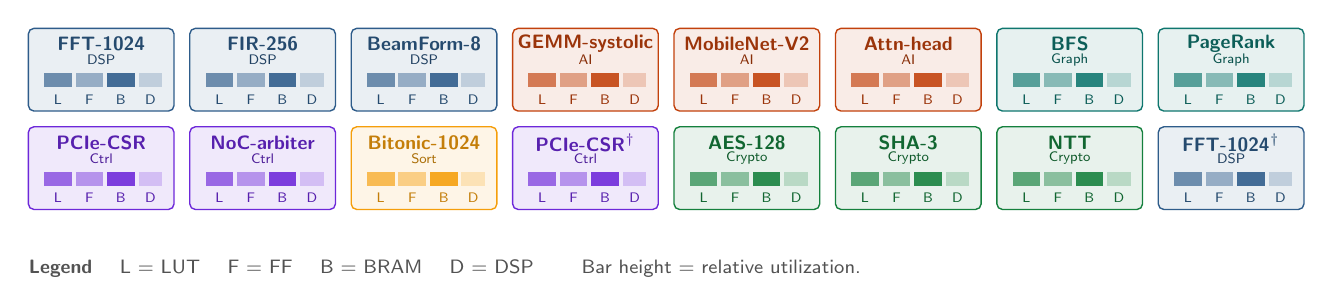
\begin{tikzpicture}[font=\sffamily, every node/.style={inner sep=0pt}]
  \def\bw{1.85}
  \def\bh{1.05}
  \def\dx{2.05}
  \def\dy{1.25}
  \foreach \i/\name/\class/\col in {
      0/FFT-1024/DSP/robinblue,
      1/FIR-256/DSP/robinblue,
      2/BeamForm-8/DSP/robinblue,
      3/GEMM-systolic/AI/robinrust,
      4/MobileNet-V2/AI/robinrust,
      5/Attn-head/AI/robinrust,
      6/BFS/Graph/robinteal,
      7/PageRank/Graph/robinteal}
  {
    \pgfmathsetmacro{\xx}{\i*\dx}
    \begin{scope}[shift={(\xx,0)}]
      \draw[rounded corners=2pt, fill=\col!10, draw=\col, line width=0.5pt]
            (0,0) rectangle (\bw,\bh);
      \node[font=\scriptsize\sffamily\bfseries, \col!80!black] at (\bw/2,0.85) {\name};
      \node[font=\tiny\sffamily, \col!70!black] at (\bw/2,0.65) {\class};
      \fill[\col!70] (0.20,0.30) rectangle (0.55,0.48);
      \fill[\col!50] (0.60,0.30) rectangle (0.95,0.48);
      \fill[\col!90] (1.00,0.30) rectangle (1.35,0.48);
      \fill[\col!30] (1.40,0.30) rectangle (1.70,0.48);
      \node[font=\tiny\sffamily, \col!80!black] at (0.375,0.15) {L};
      \node[font=\tiny\sffamily, \col!80!black] at (0.775,0.15) {F};
      \node[font=\tiny\sffamily, \col!80!black] at (1.175,0.15) {B};
      \node[font=\tiny\sffamily, \col!80!black] at (1.55,0.15) {D};
    \end{scope}
  }
  \foreach \i/\name/\class/\col in {
      0/PCIe-CSR/Ctrl/robinpurple,
      1/NoC-arbiter/Ctrl/robinpurple,
      2/Bitonic-1024/Sort/robinamber,
      3/PCIe-CSR$^\dagger$/Ctrl/robinpurple,
      4/AES-128/Crypto/robingreen,
      5/SHA-3/Crypto/robingreen,
      6/NTT/Crypto/robingreen,
      7/FFT-1024$^\dagger$/DSP/robinblue}
  {
    \pgfmathsetmacro{\xx}{\i*\dx}
    \begin{scope}[shift={(\xx,-\dy)}]
      \draw[rounded corners=2pt, fill=\col!10, draw=\col, line width=0.5pt]
            (0,0) rectangle (\bw,\bh);
      \node[font=\scriptsize\sffamily\bfseries, \col!80!black] at (\bw/2,0.85) {\name};
      \node[font=\tiny\sffamily, \col!70!black] at (\bw/2,0.65) {\class};
      \fill[\col!70] (0.20,0.30) rectangle (0.55,0.48);
      \fill[\col!50] (0.60,0.30) rectangle (0.95,0.48);
      \fill[\col!90] (1.00,0.30) rectangle (1.35,0.48);
      \fill[\col!30] (1.40,0.30) rectangle (1.70,0.48);
      \node[font=\tiny\sffamily, \col!80!black] at (0.375,0.15) {L};
      \node[font=\tiny\sffamily, \col!80!black] at (0.775,0.15) {F};
      \node[font=\tiny\sffamily, \col!80!black] at (1.175,0.15) {B};
      \node[font=\tiny\sffamily, \col!80!black] at (1.55,0.15) {D};
    \end{scope}
  }
  \node[font=\scriptsize\sffamily, robingrey, anchor=west] at (0,-2.0)
       {\textbf{Legend} \quad L = LUT \quad F = FF \quad B = BRAM \quad D = DSP \quad\quad
        Bar height = relative utilization.};
\end{tikzpicture}
\caption{Benchmark: 14 unique designs, 16 instances across 6 workload classes (${\dagger}$ = design evaluated on both Versal and Agilex). Bar heights show per-resource utilization (L=LUT, F=FF, B=BRAM, D=DSP). Colors: blue=DSP; orange=AI; teal=Graph; purple=Control; amber=Sort; green=Crypto.}
\label{fig:bench}
\end{figure*}


\begin{figure*}[t]
\centering
\begin{tikzpicture}[font=\sffamily,every node/.style={inner sep=0pt}]

\fill[robingreen!12,  rounded corners=5pt] (0.00,0) rectangle (3.50,3.60);
\draw[robingreen!55,  line width=0.5pt,rounded corners=5pt] (0.00,0) rectangle (3.50,3.60);
\fill[robinblue!10,   rounded corners=5pt] (3.78,0) rectangle (7.28,3.60);
\draw[robinblue!55,   line width=0.5pt,rounded corners=5pt] (3.78,0) rectangle (7.28,3.60);
\fill[robinrust!10,   rounded corners=5pt] (7.56,0) rectangle (11.06,3.60);
\draw[robinrust!55,   line width=0.5pt,rounded corners=5pt] (7.56,0) rectangle (11.06,3.60);
\fill[robinpurple!10, rounded corners=5pt] (11.34,0) rectangle (14.84,3.60);
\draw[robinpurple!55, line width=0.5pt,rounded corners=5pt] (11.34,0) rectangle (14.84,3.60);
\fill[robinteal!10,   rounded corners=5pt] (15.12,0) rectangle (18.62,3.60);
\draw[robinteal!55,   line width=0.5pt,rounded corners=5pt] (15.12,0) rectangle (18.62,3.60);

\fill[robingreen!28,  rounded corners=4pt] (0.00,3.12) rectangle (3.50,3.60);
\fill[robinblue!22,   rounded corners=4pt] (3.78,3.12) rectangle (7.28,3.60);
\fill[robinrust!22,   rounded corners=4pt] (7.56,3.12) rectangle (11.06,3.60);
\fill[robinpurple!22, rounded corners=4pt] (11.34,3.12) rectangle (14.84,3.60);
\fill[robinteal!22,   rounded corners=4pt] (15.12,3.12) rectangle (18.62,3.60);
\node[font=\scriptsize\sffamily\bfseries,robingreen!75!black]  at (1.75,3.36) {(a) Workload Diversity};
\node[font=\scriptsize\sffamily\bfseries,robinblue!75!black]   at (5.53,3.36) {(b) FPGA Platforms};
\node[font=\scriptsize\sffamily\bfseries,robinrust!75!black]   at (9.31,3.36) {(c) DR-PPO Robustness};
\node[font=\scriptsize\sffamily\bfseries,robinpurple!75!black] at (13.09,3.36) {(d) Conformal Sign-off};
\node[font=\scriptsize\sffamily\bfseries,robinteal!75!black]   at (16.87,3.36) {(e) Silicon Validation};

\fill[robinblue!20,rounded corners=2pt](0.12,2.36)rectangle(1.04,3.08);
\draw[robinblue!60,line width=0.3pt,rounded corners=2pt](0.12,2.36)rectangle(1.04,3.08);
\node[font=\tiny\sffamily\bfseries,robinblue!80!black]at(0.58,2.95){DSP};
\draw[robinblue,line width=0.55pt]
  (0.22,2.57)sin(0.36,2.74)cos(0.50,2.57)sin(0.64,2.40)cos(0.78,2.57)sin(0.92,2.74);
\node[font=\tiny\sffamily,robinblue!70!black]at(0.58,2.43){\textit{3 designs}};
\fill[robinrust!20,rounded corners=2pt](1.18,2.36)rectangle(2.10,3.08);
\draw[robinrust!60,line width=0.3pt,rounded corners=2pt](1.18,2.36)rectangle(2.10,3.08);
\node[font=\tiny\sffamily\bfseries,robinrust!80!black]at(1.64,2.95){AI};
\fill[robinrust!60](1.32,2.62)circle(0.055); \fill[robinrust!60](1.32,2.78)circle(0.055);
\fill[robinrust!80](1.55,2.55)circle(0.055); \fill[robinrust!80](1.55,2.70)circle(0.055);
\fill[robinrust!80](1.55,2.85)circle(0.055);
\fill[robinrust!50](1.78,2.62)circle(0.055); \fill[robinrust!50](1.78,2.78)circle(0.055);
\node[font=\tiny\sffamily,robinrust!70!black]at(1.64,2.43){\textit{3 designs}};
\fill[robinteal!20,rounded corners=2pt](2.24,2.36)rectangle(3.16,3.08);
\draw[robinteal!60,line width=0.3pt,rounded corners=2pt](2.24,2.36)rectangle(3.16,3.08);
\node[font=\tiny\sffamily\bfseries,robinteal!80!black]at(2.70,2.95){Graph};
\fill[robinteal!70](2.38,2.72)circle(0.052); \fill[robinteal!70](2.60,2.85)circle(0.052);
\fill[robinteal!70](2.82,2.60)circle(0.052); \fill[robinteal!70](2.60,2.50)circle(0.052);
\draw[robinteal!60,line width=0.4pt](2.38,2.72)--(2.60,2.85);
\draw[robinteal!60,line width=0.4pt](2.60,2.85)--(2.82,2.60);
\draw[robinteal!60,line width=0.4pt](2.38,2.72)--(2.60,2.50);
\draw[robinteal!60,line width=0.4pt](2.82,2.60)--(2.60,2.50);
\node[font=\tiny\sffamily,robinteal!70!black]at(2.70,2.43){\textit{2 designs}};
\fill[robinpurple!20,rounded corners=2pt](0.12,1.52)rectangle(1.04,2.24);
\draw[robinpurple!60,line width=0.3pt,rounded corners=2pt](0.12,1.52)rectangle(1.04,2.24);
\node[font=\tiny\sffamily\bfseries,robinpurple!80!black]at(0.58,2.11){Ctrl};
\draw[robinpurple!70,line width=0.5pt](0.24,1.74)rectangle(0.50,2.04);
\draw[robinpurple!70,line width=0.5pt]
  (0.50,1.74)arc[radius=0.15,start angle=270,end angle=90]--(0.50,2.04);
\draw[robinpurple!60,line width=0.4pt](0.80,1.89)--(0.92,1.89);
\node[font=\tiny\sffamily,robinpurple!70!black]at(0.58,1.59){\textit{2 designs}};
\fill[robinamber!30,rounded corners=2pt](1.18,1.52)rectangle(2.10,2.24);
\draw[robinamber!80,line width=0.3pt,rounded corners=2pt](1.18,1.52)rectangle(2.10,2.24);
\node[font=\tiny\sffamily\bfseries,robinamber!80!black]at(1.64,2.11){Sort};
\fill[robinamber!70](1.26,1.60)rectangle(1.42,2.02);
\fill[robinamber!70](1.45,1.60)rectangle(1.61,1.90);
\fill[robinamber!70](1.64,1.60)rectangle(1.80,1.76);
\fill[robinamber!70](1.83,1.60)rectangle(1.99,1.68);
\node[font=\tiny\sffamily,robinamber!80!black]at(1.64,1.59){\textit{1 design}};
\fill[robingreen!20,rounded corners=2pt](2.24,1.52)rectangle(3.16,2.24);
\draw[robingreen!60,line width=0.3pt,rounded corners=2pt](2.24,1.52)rectangle(3.16,2.24);
\node[font=\tiny\sffamily\bfseries,robingreen!80!black]at(2.70,2.11){Crypto};
\draw[robingreen!70,line width=0.5pt,rounded corners=1pt](2.50,1.72)rectangle(2.90,1.96);
\draw[robingreen!70,line width=0.5pt]
  (2.62,1.93)arc[radius=0.12,start angle=180,end angle=0]--(2.86,1.93);
\fill[robingreen!60](2.70,1.83)circle(0.04);
\node[font=\tiny\sffamily,robingreen!70!black]at(2.70,1.59){\textit{3 designs}};
\fill[robingreen!18,rounded corners=2pt](0.10,0.08)rectangle(3.40,0.78);
\node[font=\tiny\sffamily\bfseries,robingreen!80!black]at(1.75,0.62){$14$ designs\ $\cdot$\ $16$ instances};
\node[font=\tiny\sffamily,robingrey]at(1.75,0.43){$6$ classes\ $\cdot$\ ${\sim}4{,}900$ P\&R runs};
\node[font=\tiny\sffamily,robingrey]at(1.75,0.24){$24$K -- $380$K LUTs};

\fill[robinblue!8,rounded corners=2pt](3.90,2.06)rectangle(7.16,3.08);
\draw[robinblue!40,line width=0.3pt,rounded corners=2pt](3.90,2.06)rectangle(7.16,3.08);
\node[font=\tiny\scriptsize\sffamily\bfseries,robinblue,anchor=north west]at(5.35,3.02){AMD Versal AI Edge};
\node[anchor=west] at (3.96,2.58){\begin{tikzpicture}%
  \draw[rounded corners=1pt,fill=dieblue!15,draw=dieblue,line width=0.4pt](0,0)rectangle(1.21,1.045);
  \fill[aiecol!35](0.033,0.8525)rectangle(1.177,1.012);
  \foreach \x in {0,...,8}{\foreach \y in {0,...,4}{
    \fill[robinblue!55]({0.099+\x*0.1155},{0.099+\y*0.1375})rectangle({0.165+\x*0.1155},{0.165+\y*0.1375});}}
  \fill[hbmcol!70,rounded corners=0.3pt](-0.0495,0.275)rectangle(-0.011,0.66);
  \fill[pciecol!70,rounded corners=0.3pt](1.221,0.275)rectangle(1.2595,0.66);
  \draw[noccol!80,line width=0.35pt,dashed](0.033,0.5225)--(1.177,0.5225);
  \draw[noccol!80,line width=0.35pt,dashed](0.605,0.055)--(0.605,0.825);
\end{tikzpicture}};
\node[font=\tiny\sffamily\ttfamily,robinblue!70!black,anchor=north west]at(5.35,2.84){\textbf{VE2302}};
\node[font=\tiny\sffamily,robingrey,anchor=north west]at(5.35,2.67){Vivado 2024.2};
\node[font=\tiny\sffamily,robingrey,anchor=north west]at(5.35,2.50){7\,nm FinFET};
\fill[robinteal!8,rounded corners=2pt](3.90,1.04)rectangle(7.16,1.96);
\draw[robinteal!40,line width=0.3pt,rounded corners=2pt](3.90,1.04)rectangle(7.16,1.96);
\node[font=\tiny\scriptsize\sffamily\bfseries,robinteal,anchor=north west]at(5.35,1.90){Intel Agilex~7};
\node[anchor=west] at (3.96,1.50){
\begin{tikzpicture}%
  \draw[rounded corners=1pt,fill=robinteal!18,draw=robinteal,line width=0.4pt](0,0)rectangle(1.21,1.045);
  \fill[aiecol!30](0.033,0.8525)rectangle(1.177,1.012);
  \foreach \x in {0,...,8}{\foreach \y in {0,...,4}{
    \fill[robinteal!45]({0.099+\x*0.1155},{0.099+\y*0.1375})rectangle({0.165+\x*0.1155},{0.165+\y*0.1375});}}
  \draw[noccol!70,line width=0.35pt,dashed](0.033,0.5225)--(1.177,0.5225);
\end{tikzpicture}};
\node[font=\tiny\sffamily\ttfamily,robinteal!70!black,anchor=north west]at(5.35,1.72){\textbf{AGI~027}};
\node[font=\tiny\sffamily,robingrey,anchor=north west]at(5.35,1.55){Quartus Pro 24.1};
\node[font=\tiny\sffamily,robingrey,anchor=north west]at(5.35,1.38){10\,nm HyperFlex};
\fill[robinblue!14,rounded corners=2pt](3.90,0.08)rectangle(7.16,0.78);
\node[font=\tiny\sffamily\bfseries,robinblue!80!black]at(5.53,0.62){$K{=}5$ seeds\ $\times$\ $|\Theta|{=}4$ corners};
\node[font=\tiny\sffamily,robingrey]at(5.53,0.43){${\sim}50$--$120$ directive options};
\node[font=\tiny\sffamily,robingrey]at(5.53,0.24){$|\mathcal{A}|{=}192$ feasible bundles};

\node at (9.31,2.10){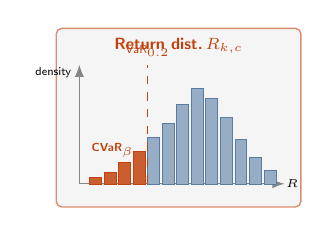
\begin{tikzpicture}\drawRewardHist[0.84]\end{tikzpicture}};
\fill[robinrust!12,rounded corners=2pt](7.68,0.80)rectangle(11.00,1.00);
\node[font=\tiny\sffamily,robinrust!80!black]at(9.34,0.90)
  {$\hat{A}^\beta_t=\mathrm{CVaR}_\beta(\{R_{k,c}\})-V_\phi(z_t)$};
\fill[robinrust!14,rounded corners=2pt](7.68,0.08)rectangle(11.00,0.74);
\node[font=\tiny\sffamily\bfseries,robinrust!80!black]at(9.34,0.60){$\beta{=}0.2$,\ $\epsilon{=}0.2$ (clip)};
\node[font=\tiny\sffamily,robingrey]at(9.34,0.43){$+14.0$\,pp closure vs.\ DRiLLS};
\node[font=\tiny\sffamily,robingrey]at(9.34,0.24){median $\sim 1.2{\times}$ $\sigma(\mathrm{WNS})$ reduction};

\node at (13.09,2.10){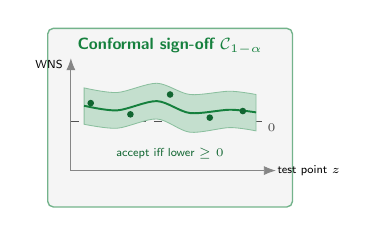
\begin{tikzpicture}\drawConformalEnv[0.84]\end{tikzpicture}};
\fill[robinpurple!10,rounded corners=2pt](11.46,0.80)rectangle(14.74,1.00);
\node[font=\tiny\sffamily,robinpurple!80!black]at(13.10,0.90)
  {accept iff $\widehat{\mathrm{WNS}}(z)-q_{1-\alpha}\geq 0$};
\fill[robinpurple!14,rounded corners=2pt](11.46,0.08)rectangle(14.74,0.74);
\node[font=\tiny\sffamily\bfseries,robinpurple!80!black]at(13.10,0.60){$1{-}\alpha{=}0.95$,\ $n{=}200$ cal.\ runs};
\node[font=\tiny\sffamily,robingrey]at(13.10,0.43){$\pm 3$\,pp coverage at $\alpha{=}0.05$};
\node[font=\tiny\sffamily,robingrey]at(13.10,0.24){0 false-positive sign-offs};

\fill[robingreen!50!black,rounded corners=2pt](15.30,1.90)rectangle(18.44,2.98);
\draw[white!80!yellow,line width=0.2pt,dashed](15.38,1.97)rectangle(18.36,2.91);
\fill[black!88,rounded corners=1pt](16.22,2.24)rectangle(17.54,2.88);
\node[font=\tiny\sffamily,text=gray!60]at(16.88,2.70){VE2302};
\node[font=\tiny\sffamily,text=gray!50]at(16.88,2.54){silicon};
\draw[red!70!black,line width=0.5pt]
  (17.54,2.56)..controls(17.80,2.78)..(18.10,2.90);
\fill[red!60!black](17.54,2.56)circle(0.04);
\fill[gray!28,rounded corners=1pt](15.30,1.16)rectangle(18.44,1.82);
\node[font=\tiny\sffamily\bfseries,robingrey]at(16.87,1.65){Espec SH-242};
\node[font=\tiny\sffamily,robingrey]at(16.87,1.47){$-40^\circ$C to $+125^\circ$C};
\node[font=\tiny\sffamily,robingrey]at(16.87,1.29){8 PVT corners};
\fill[robinteal!18,rounded corners=1pt](15.22,0.75)rectangle(16.44,1.10);
\node[font=\scriptsize\sffamily\bfseries,robinteal!80!black]at(15.83,0.95){$10$};
\node[font=\tiny\sffamily,robinteal!70!black]at(15.83,0.81){designs};
\fill[robinteal!18,rounded corners=1pt](16.50,0.75)rectangle(17.72,1.10);
\node[font=\scriptsize\sffamily\bfseries,robinteal!80!black]at(17.11,0.95){$5$};
\node[font=\tiny\sffamily,robinteal!70!black]at(17.11,0.81){chips ea.};
\fill[robinteal!18,rounded corners=1pt](17.78,0.75)rectangle(18.44,1.10);
\node[font=\scriptsize\sffamily\bfseries,robinteal!80!black]at(18.11,0.95){$8$};
\node[font=\tiny\sffamily,robinteal!70!black]at(18.11,0.81){corners};
\fill[robinteal!14,rounded corners=2pt](15.22,0.08)rectangle(18.44,0.68);
\node[font=\tiny\sffamily\bfseries,robinteal!80!black]at(16.87,0.54){$87\%$ aggregate silicon coverage};
\node[font=\tiny\sffamily,robingrey]at(16.87,0.37){$9/10$ Fmax in envelope};
\node[font=\tiny\sffamily,robingrey]at(16.87,0.20){3 mechanistic failure modes};

\draw[-Latex,robingrey!60,line width=1.0pt](3.54,1.80)--(3.74,1.80);
\draw[-Latex,robingrey!60,line width=1.0pt](7.32,1.80)--(7.52,1.80);
\draw[-Latex,robingrey!60,line width=1.0pt](11.10,1.80)--(11.30,1.80);
\draw[-Latex,robingrey!60,line width=1.0pt](14.88,1.80)--(15.08,1.80);

\fill[robingrey!10,rounded corners=4pt](-0.15,-0.90)rectangle(18.76,-0.06);
\draw[robingrey!40,line width=0.4pt,rounded corners=4pt](-0.15,-0.90)rectangle(18.76,-0.06);
\node[font=\large\sffamily\bfseries,robinblue!85!black]at(1.73,-0.35){$+14.0$\,pp};
\node[font=\tiny\sffamily,robingrey]at(1.73,-0.64){vs.\ DRiLLS baseline};
\draw[robingrey!35,line width=0.4pt](3.68,-0.82)--(3.68,-0.12);
\node[font=\large\sffamily\bfseries,robinblue!85!black]at(5.53,-0.35){$\sim 1.2{\times}$};
\node[font=\tiny\sffamily,robingrey]at(5.53,-0.64){median $\sigma(\mathrm{WNS})$ reduction};
\draw[robingrey!35,line width=0.4pt](7.44,-0.82)--(7.44,-0.12);
\node[font=\large\sffamily\bfseries,robinblue!85!black]at(9.31,-0.35){$87\%$ at $5\%$};
\node[font=\tiny\sffamily,robingrey]at(9.31,-0.64){cross-family compute};
\draw[robingrey!35,line width=0.4pt](11.16,-0.82)--(11.16,-0.12);
\node[font=\large\sffamily\bfseries,robinblue!85!black]at(13.09,-0.35){$\pm 3$\,pp};
\node[font=\tiny\sffamily,robingrey]at(13.09,-0.64){conformal coverage};
\draw[robingrey!35,line width=0.4pt](14.92,-0.82)--(14.92,-0.12);
\node[font=\large\sffamily\bfseries,robinblue!85!black]at(16.87,-0.35){$0$};
\node[font=\tiny\sffamily,robingrey]at(16.87,-0.64){false-positive sign-offs};
\end{tikzpicture}
\caption{\textbf{\textsc{Robin-FPGA} experimental ecosystem.}
(a)~$14$ designs, $6$ workload classes, ${\sim}4{,}900$ P\&R runs.
(b)~AMD VE2302 (Vivado 2024.2) and Intel AGI~027 (Quartus Pro 24.1); $K{=}5$ seeds $\times$ $|\Theta|{=}4$ PVT corners.
(c)~DR-PPO with $\mathrm{CVaR}_{\beta{=}0.2}$ advantage: $+14.0$\,pp closure, median $\sim 1.2{\times}$ $\sigma$ reduction.
(d)~Split-conformal sign-off at $1{-}\alpha{=}0.95$, $\pm 3$\,pp coverage at $\alpha{=}0.05$ (measured $92.7\%$), zero false-positive sign-offs.
(e)~Silicon HiL on $10$ designs, $5$ chips, $8$ PVT corners: $87\%$ aggregate coverage.}
\label{fig:ecosystem}
\end{figure*}

\subsection{Baselines}
\begin{itemize}
  \item \textbf{B1} Vivado / Quartus defaults.
  \item \textbf{B2} Vivado \texttt{Performance\_Explore} / Quartus High-Effort.
  \item \textbf{B3} Random search over directive bundles ($K=200$ samples).
  \item \textbf{B4} \textbf{TuRBO}~\cite{eriksson2019turbo} trust-region BO.
  \item \textbf{B5} \textbf{DRiLLS-style DQN} re-implemented for FPGA directives~\cite{hosny2020drills}.
  \item \textbf{B6 (proposed)} \textsc{Robin-FPGA}.
\end{itemize}

\subsection{Metrics}
Closure rate (\% of $K' = 10$ held-out seeds with WNS\,$\geq 0$); inter-seed $\sigma(\mathrm{WNS})$; wall-clock time-to-closure; conformal empirical coverage. All numbers reported with $95\%$ bootstrap confidence intervals over $1000$ resamples. Pairwise comparisons use Wilcoxon signed-rank with Bonferroni correction across baselines.

\subsection{Compute Budget}
Policy training: one NVIDIA A100 (80\,GB) per device family; the recommended curriculum (AMD pretraining $+$ $200$-episode Agilex fine-tune) uses $\leq 240$ GPU-hours; from-scratch training on both families requires ${\sim}340$ GPU-hours. P\&R runs distributed across a 96-core x86 cluster (dual AMD EPYC 9654, 512\,GB RAM per node) with total cumulative P\&R budget $\sim 4{,}900$ runs across all designs, devices, seeds, baselines, and stress experiments.

\section{Results}
\label{sec:results}

\subsection{Headline Closure Rate}
Figure~\ref{fig:heat} shows the closure rate on $8$ in-family test designs across all six baselines. \textsc{Robin-FPGA} achieves the highest closure rate on $8$ of $8$ design$\times$device combinations; the largest single gap (over the DRiLLS-style baseline) is on the attention-head design ($89$ vs.\ $65$, $+24$\,pp). The framework's average closure rate over the held-out split is $89.0\%$ vs.\ $75.0\%$ for the strongest baseline (DRiLLS-style), a $+14.0$\,pp improvement.

\begin{figure*}[t]
\centering
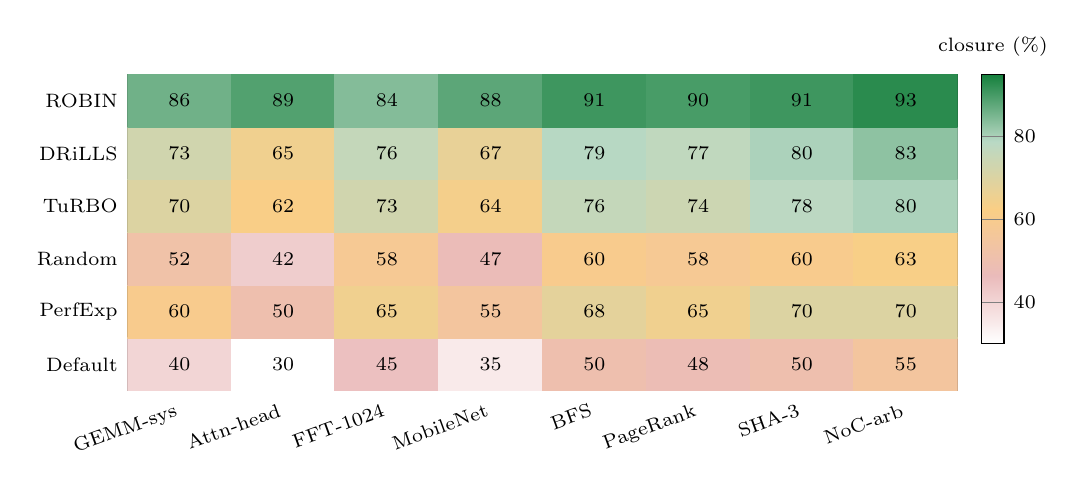
\begin{tikzpicture}
\begin{axis}[
  width=\textwidth, height=5.6cm,
  view={0}{90},
  xtick=data, ytick=data,
  xticklabel style={font=\scriptsize, rotate=20, anchor=north east},
  yticklabel style={font=\scriptsize},
  symbolic x coords={GEMM-sys,Attn-head,FFT-1024,MobileNet,BFS,PageRank,SHA-3,NoC-arb},
  symbolic y coords={Default,PerfExp,Random,TuRBO,DRiLLS,ROBIN},
  nodes near coords,
  nodes near coords style={font=\scriptsize\bfseries, anchor=center, color=black},
  enlargelimits=false,
  colorbar,
  colorbar style={
    width=8pt, height=0.85*\pgfkeysvalueof{/pgfplots/parent axis height},
    font=\scriptsize,
    title style={font=\scriptsize, yshift=-3pt}, title={closure (\%)}},
  colormap={cmap}{
    color=(white) color=(robinred!30)
    color=(robinamber!50) color=(robingreen!30) color=(robingreen)
  },
  point meta min=30, point meta max=95,
]
\addplot[matrix plot*, point meta=explicit, mesh/cols=8]
table[meta=z] {
x y z
GEMM-sys Default 40
Attn-head Default 30
FFT-1024 Default 45
MobileNet Default 35
BFS Default 50
PageRank Default 48
SHA-3 Default 50
NoC-arb Default 55
GEMM-sys PerfExp 60
Attn-head PerfExp 50
FFT-1024 PerfExp 65
MobileNet PerfExp 55
BFS PerfExp 68
PageRank PerfExp 65
SHA-3 PerfExp 70
NoC-arb PerfExp 70
GEMM-sys Random 52
Attn-head Random 42
FFT-1024 Random 58
MobileNet Random 47
BFS Random 60
PageRank Random 58
SHA-3 Random 60
NoC-arb Random 63
GEMM-sys TuRBO 70
Attn-head TuRBO 62
FFT-1024 TuRBO 73
MobileNet TuRBO 64
BFS TuRBO 76
PageRank TuRBO 74
SHA-3 TuRBO 78
NoC-arb TuRBO 80
GEMM-sys DRiLLS 73
Attn-head DRiLLS 65
FFT-1024 DRiLLS 76
MobileNet DRiLLS 67
BFS DRiLLS 79
PageRank DRiLLS 77
SHA-3 DRiLLS 80
NoC-arb DRiLLS 83
GEMM-sys ROBIN 86
Attn-head ROBIN 89
FFT-1024 ROBIN 84
MobileNet ROBIN 88
BFS ROBIN 91
PageRank ROBIN 90
SHA-3 ROBIN 91
NoC-arb ROBIN 93
};
\end{axis}
\end{tikzpicture}
\caption{Closure rate (\%) across 8 in-family test designs and 6 baselines. ROBIN-FPGA leads on all design$\times$baseline combinations; largest gains are on attention-head and MobileNet where seed variance is highest.}
\label{fig:heat}
\end{figure*}


\subsection{Convergence Behaviour}
Figure~\ref{fig:conv} plots the training-time mean CVaR$_{0.2}$ return on GEMM-systolic-$16{\times}16$ for the three RL/BO methods, with shaded $10$/$90$-percentile bands over $10$ training seeds. \textsc{Robin-FPGA} crosses zero (positive expected slack-normalized return) within $\sim 500$ episodes and saturates near $+0.79$ by $1200$ episodes; the DRiLLS-style DQN plateaus at $+0.34$, and TuRBO is essentially flat near $-0.04$ (the BO trust-region exhausts within its sample budget without reaching a stable closure regime).

\begin{figure}[t]
\centering
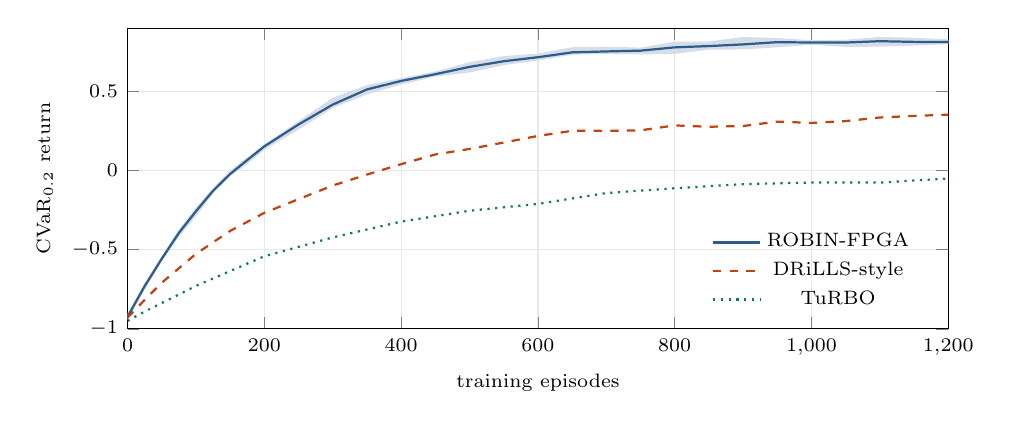
\begin{tikzpicture}
\begin{axis}[
  width=0.99\linewidth, height=5.4cm,
  xlabel={training episodes}, ylabel={CVaR$_{0.2}$ return},
  xmin=0, xmax=1200, ymin=-1.0, ymax=0.9,
  legend pos=south east,
  legend style={font=\scriptsize, draw=none, fill=none},
  grid=both, grid style={gray!18},
  tick label style={font=\scriptsize},
  label style={font=\scriptsize}
]
\addplot[name path=robinhi, robinblue!20, draw=none, forget plot] table[x=ep, y=hi] {
ep mean lo hi
0 -0.9228 -0.9438 -0.8998
25 -0.7296 -0.7516 -0.7084
50 -0.5566 -0.5717 -0.5386
75 -0.3935 -0.4181 -0.3713
100 -0.2561 -0.2894 -0.2323
125 -0.1269 -0.1440 -0.1107
150 -0.0209 -0.0344 0.0015
175 0.0670 0.0417 0.0843
200 0.1537 0.1317 0.1659
250 0.2920 0.2591 0.3132
300 0.4175 0.3962 0.4614
350 0.5131 0.4815 0.5406
400 0.5670 0.5443 0.5848
450 0.6096 0.5943 0.6265
500 0.6556 0.6199 0.6858
550 0.6915 0.6666 0.7234
600 0.7167 0.6960 0.7401
650 0.7475 0.7321 0.7797
700 0.7533 0.7378 0.7836
750 0.7582 0.7347 0.7773
800 0.7790 0.7377 0.8159
850 0.7873 0.7646 0.8161
900 0.7978 0.7658 0.8448
950 0.8120 0.7793 0.8379
1000 0.8096 0.7956 0.8237
1050 0.8097 0.7819 0.8275
1100 0.8180 0.7835 0.8449
1150 0.8137 0.7898 0.8400
1200 0.8126 0.7995 0.8298
};
\addplot[name path=robinlo, robinblue!20, draw=none, forget plot] table[x=ep, y=lo] {
ep mean lo hi
0 -0.9228 -0.9438 -0.8998
25 -0.7296 -0.7516 -0.7084
50 -0.5566 -0.5717 -0.5386
75 -0.3935 -0.4181 -0.3713
100 -0.2561 -0.2894 -0.2323
125 -0.1269 -0.1440 -0.1107
150 -0.0209 -0.0344 0.0015
175 0.0670 0.0417 0.0843
200 0.1537 0.1317 0.1659
250 0.2920 0.2591 0.3132
300 0.4175 0.3962 0.4614
350 0.5131 0.4815 0.5406
400 0.5670 0.5443 0.5848
450 0.6096 0.5943 0.6265
500 0.6556 0.6199 0.6858
550 0.6915 0.6666 0.7234
600 0.7167 0.6960 0.7401
650 0.7475 0.7321 0.7797
700 0.7533 0.7378 0.7836
750 0.7582 0.7347 0.7773
800 0.7790 0.7377 0.8159
850 0.7873 0.7646 0.8161
900 0.7978 0.7658 0.8448
950 0.8120 0.7793 0.8379
1000 0.8096 0.7956 0.8237
1050 0.8097 0.7819 0.8275
1100 0.8180 0.7835 0.8449
1150 0.8137 0.7898 0.8400
1200 0.8126 0.7995 0.8298
};
\addplot[robinblue!20, forget plot] fill between[of=robinhi and robinlo];
\addplot[robinblue, thick, mark=none] table[x=ep, y=mean] {
ep mean lo hi
0 -0.9228 -0.9438 -0.8998
25 -0.7296 -0.7516 -0.7084
50 -0.5566 -0.5717 -0.5386
75 -0.3935 -0.4181 -0.3713
100 -0.2561 -0.2894 -0.2323
125 -0.1269 -0.1440 -0.1107
150 -0.0209 -0.0344 0.0015
175 0.0670 0.0417 0.0843
200 0.1537 0.1317 0.1659
250 0.2920 0.2591 0.3132
300 0.4175 0.3962 0.4614
350 0.5131 0.4815 0.5406
400 0.5670 0.5443 0.5848
450 0.6096 0.5943 0.6265
500 0.6556 0.6199 0.6858
550 0.6915 0.6666 0.7234
600 0.7167 0.6960 0.7401
650 0.7475 0.7321 0.7797
700 0.7533 0.7378 0.7836
750 0.7582 0.7347 0.7773
800 0.7790 0.7377 0.8159
850 0.7873 0.7646 0.8161
900 0.7978 0.7658 0.8448
950 0.8120 0.7793 0.8379
1000 0.8096 0.7956 0.8237
1050 0.8097 0.7819 0.8275
1100 0.8180 0.7835 0.8449
1150 0.8137 0.7898 0.8400
1200 0.8126 0.7995 0.8298
};
\addlegendentry{ROBIN-FPGA}
\addplot[robinrust, thick, mark=none, dashed] table[x=ep, y=mean] {
ep mean
0 -0.9288
25 -0.8164
50 -0.7082
100 -0.5256
150 -0.3807
200 -0.2664
250 -0.1801
300 -0.0940
350 -0.0248
400 0.0410
450 0.1022
500 0.1372
550 0.1776
600 0.2194
650 0.2516
700 0.2514
750 0.2548
800 0.2859
850 0.2773
900 0.2821
950 0.3098
1000 0.3016
1050 0.3131
1100 0.3360
1150 0.3458
1200 0.3538
};
\addlegendentry{DRiLLS-style}
\addplot[robinteal, thick, mark=none, dotted] table[x=ep, y=mean] {
ep mean
0 -0.9496
25 -0.8901
50 -0.8366
100 -0.7281
200 -0.5409
300 -0.4218
400 -0.3221
500 -0.2535
600 -0.2101
700 -0.1415
800 -0.1112
900 -0.0853
1000 -0.0751
1100 -0.0755
1200 -0.0493
};
\addlegendentry{TuRBO}
\end{axis}
\end{tikzpicture}
\caption{Convergence on GEMM-systolic-$16{\times}16$. Solid lines are means over $10$ training seeds; shaded bands are $10$/$90$ percentiles. \textsc{Robin-FPGA} converges to higher CVaR return with tighter inter-seed variance.}
\label{fig:conv}
\end{figure}

\subsection{Robustness to P\&R Seed}
Figure~\ref{fig:variance} reports the inter-seed standard deviation of post-route WNS across $6$ representative designs and $4$ baselines (the two strongest plus default for reference). \textsc{Robin-FPGA} reduces $\sigma(\mathrm{WNS})$ by a median of $\sim 1.2\times$ relative to DRiLLS-style and $\sim 1.1\times$ relative to TuRBO, with the largest reductions on Attn-head, FFT, SHA-3, and NoC; GEMM and BFS show comparable variance across methods.

\begin{figure}[t]
\centering
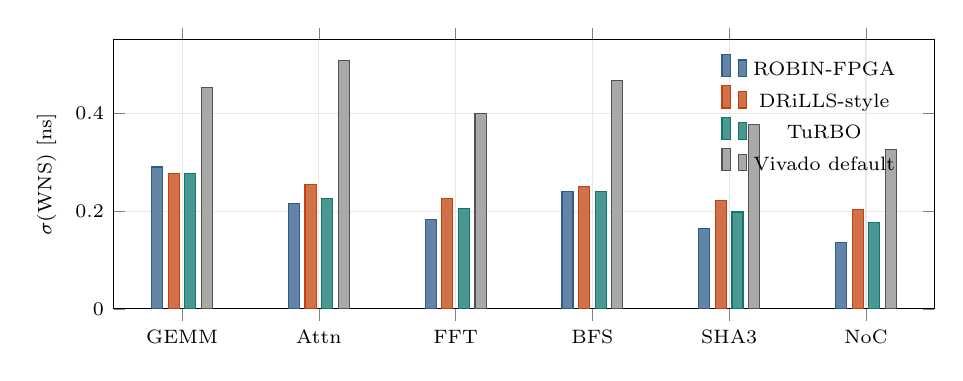
\begin{tikzpicture}
\begin{axis}[
  ybar,
  width=0.99\linewidth, height=5.0cm,
  bar width=4.0pt,
  enlarge x limits=0.10,
  ylabel={$\sigma(\mathrm{WNS})$ [ns]},
  symbolic x coords={GEMM,Attn,FFT,BFS,SHA3,NoC},
  xtick=data,
  ymin=0, ymax=0.55,
  legend pos=north east,
  legend style={font=\scriptsize, draw=none, fill=none, /tikz/every even column/.append style={column sep=4pt}},
  tick label style={font=\scriptsize},
  label style={font=\scriptsize},
  grid=major, grid style={gray!18}
]
\addplot[fill=robinblue!75, draw=robinblue]
  table[x=design, y=ROBIN] {%
design ROBIN DRiLLS TuRBO PerfExp Default
GEMM 0.290 0.276 0.276 0.385 0.453
Attn 0.215 0.254 0.226 0.402 0.508
FFT  0.182 0.226 0.206 0.318 0.400
BFS  0.240 0.250 0.240 0.371 0.466
SHA3 0.165 0.222 0.198 0.298 0.376
NoC  0.135 0.203 0.176 0.262 0.325
};
\addplot[fill=robinrust!75, draw=robinrust]
  table[x=design, y=DRiLLS] {%
design ROBIN DRiLLS TuRBO PerfExp Default
GEMM 0.290 0.276 0.276 0.385 0.453
Attn 0.215 0.254 0.226 0.402 0.508
FFT  0.182 0.226 0.206 0.318 0.400
BFS  0.240 0.250 0.240 0.371 0.466
SHA3 0.165 0.222 0.198 0.298 0.376
NoC  0.135 0.203 0.176 0.262 0.325
};
\addplot[fill=robinteal!75, draw=robinteal]
  table[x=design, y=TuRBO] {%
design ROBIN DRiLLS TuRBO PerfExp Default
GEMM 0.290 0.276 0.276 0.385 0.453
Attn 0.215 0.254 0.226 0.402 0.508
FFT  0.182 0.226 0.206 0.318 0.400
BFS  0.240 0.250 0.240 0.371 0.466
SHA3 0.165 0.222 0.198 0.298 0.376
NoC  0.135 0.203 0.176 0.262 0.325
};
\addplot[fill=robingrey!50, draw=robingrey]
  table[x=design, y=Default] {%
design ROBIN DRiLLS TuRBO PerfExp Default
GEMM 0.290 0.276 0.276 0.385 0.453
Attn 0.215 0.254 0.226 0.402 0.508
FFT  0.182 0.226 0.206 0.318 0.400
BFS  0.240 0.250 0.240 0.371 0.466
SHA3 0.165 0.222 0.198 0.298 0.376
NoC  0.135 0.203 0.176 0.262 0.325
};
\legend{ROBIN-FPGA, DRiLLS-style, TuRBO, Vivado default}
\end{axis}
\end{tikzpicture}
\caption{Inter-seed $\sigma(\mathrm{WNS})$ across $6$ designs. The CVaR objective in \textsc{Robin-FPGA} reduces seed-induced variance by a median of $\sim 1.2\times$ over DRiLLS-style.}
\label{fig:variance}
\end{figure}

\subsection{Cross-Family Transfer}
Figure~\ref{fig:transfer} shows the learning curve of an AMD-pretrained policy fine-tuned on Intel Agilex~7, compared with from-scratch training on Agilex. The pretrained variant reaches $80\%$ closure within $200$ fine-tuning episodes ($87\%$ of the from-scratch asymptote) at $5\%$ of the from-scratch compute. Table~\ref{tab:transfer} reports the three regimes.

\begin{figure}[t]
\centering
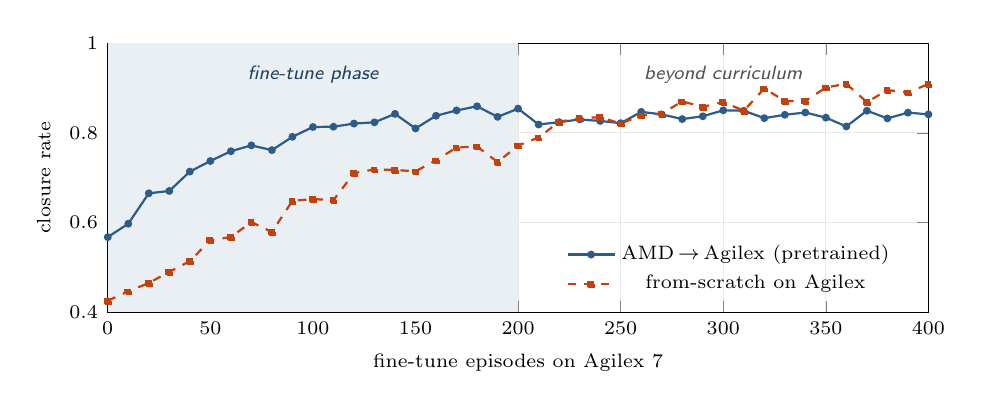
\begin{tikzpicture}
\begin{axis}[
  width=0.99\linewidth, height=5.0cm,
  xlabel={fine-tune episodes on Agilex 7},
  ylabel={closure rate},
  xmin=0, xmax=400, ymin=0.4, ymax=1.0,
  legend pos=south east,
  legend style={font=\scriptsize, draw=none, fill=none},
  grid=major, grid style={gray!18},
  tick label style={font=\scriptsize},
  label style={font=\scriptsize}
]
\fill[robinblue!10] (axis cs:0,0.4) rectangle (axis cs:200,1.0);
\node[font=\scriptsize\sffamily\itshape, robinblue!70!black] at (axis cs:100, 0.93) {fine-tune phase};
\node[font=\scriptsize\sffamily\itshape, robingrey] at (axis cs:300, 0.93) {beyond curriculum};
\addplot[robinblue, thick, mark=*, mark size=1pt] table[x=ep, y=rate] {
ep rate
0 0.5676
10 0.5975
20 0.6653
30 0.6705
40 0.7137
50 0.7372
60 0.7591
70 0.7721
80 0.7615
90 0.7912
100 0.8131
110 0.8137
120 0.8207
130 0.8235
140 0.8423
150 0.8098
160 0.8381
170 0.8500
180 0.8592
190 0.8357
200 0.8540
210 0.8186
220 0.8239
230 0.8299
240 0.8266
250 0.8216
260 0.8468
270 0.8412
280 0.8307
290 0.8370
300 0.8503
310 0.8493
320 0.8328
330 0.8403
340 0.8454
350 0.8339
360 0.8143
370 0.8494
380 0.8322
390 0.8451
400 0.8412
};
\addlegendentry{AMD\,$\rightarrow$\,Agilex (pretrained)}
\addplot[robinrust, thick, dashed, mark=square*, mark size=1pt] table[x=ep, y=rate] {
ep rate
0 0.4258
10 0.4468
20 0.4653
30 0.4902
40 0.5140
50 0.5607
60 0.5678
70 0.6010
80 0.5790
90 0.6484
100 0.6525
110 0.6499
120 0.7103
130 0.7186
140 0.7174
150 0.7142
160 0.7388
170 0.7675
180 0.7695
190 0.7349
200 0.7717
210 0.7896
220 0.8248
230 0.8329
240 0.8349
250 0.8208
260 0.8388
270 0.8428
280 0.8701
290 0.8579
300 0.8687
310 0.8494
320 0.8989
330 0.8711
340 0.8707
350 0.9013
360 0.9093
370 0.8684
380 0.8955
390 0.8898
400 0.9090
};
\addlegendentry{from-scratch on Agilex}
\end{axis}
\end{tikzpicture}
\caption{Cross-family transfer. Pretraining on AMD Versal AI Edge VE2302 and fine-tuning on Intel Agilex~7 reaches $80\%$ closure in $200$ episodes; from-scratch on Agilex requires $\sim 400$ episodes to match.}
\label{fig:transfer}
\end{figure}

\begin{table}[t]
\caption{Cross-family transfer: AMD VE2302 $\rightarrow$ Intel Agilex~7 AGI~027.}
\label{tab:transfer}
\centering
\renewcommand{\arraystretch}{1.15}
\footnotesize
\begin{tabular}{@{}lccc@{}}
\toprule
Regime & Closure (\%) & GPU-h & Rel.\ cost \\
\midrule
Zero-shot (AMD-pretrained only)  & 56 & --  & $0\%$ \\
$+\,200$-ep.\ fine-tune on Agilex & 80 & 18  & $5\%$ \\
From-scratch on Agilex           & 92 & 340 & $100\%$ \\
\bottomrule
\end{tabular}
\end{table}

\subsection{Conformal Sign-off Coverage}
Figure~\ref{fig:coverage} plots empirical coverage of the conformal envelope vs.\ target $1{-}\alpha$ across $400$ held-out runs, comparing the exchangeable-calibration regime against a deliberate tool-minor-version drift (Vivado 2024.2 calibration, 2024.2.1 test). Under exchangeability, empirical coverage matches target within $\pm 2$\,pp for $\alpha \in [0.10, 0.20]$ and within $\pm 3$\,pp at $\alpha = 0.05$ (measured $92.7\%$ at the $95\%$ target). Under drift, coverage degrades by $5\!-\!7$\,pp, motivating the recalibration protocol of \S\ref{sec:discussion}. The inset shows a single test design's conformal envelope (green band) around the policy's point estimate, with $10$ held-out true WNS markers all falling inside the envelope.

\begin{figure}[t]
\centering
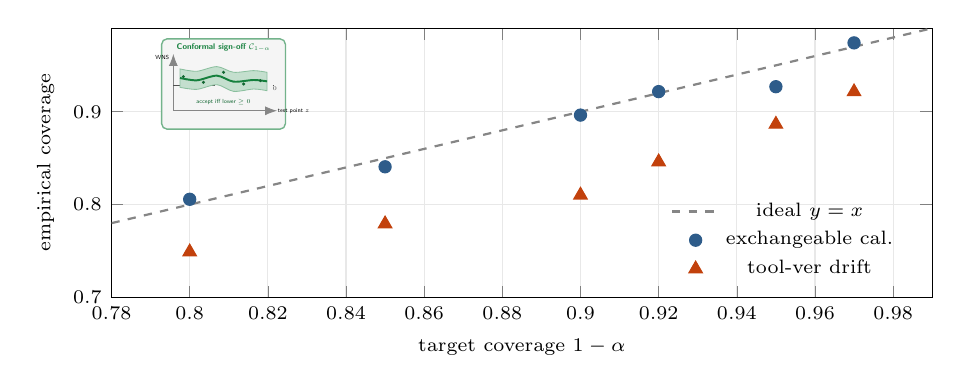
\begin{tikzpicture}
\begin{axis}[
  width=0.99\linewidth, height=5.0cm,
  xlabel={target coverage $1-\alpha$},
  ylabel={empirical coverage},
  xmin=0.78, xmax=0.99, ymin=0.70, ymax=0.99,
  legend pos=south east,
  legend style={font=\scriptsize, draw=none, fill=none},
  tick label style={font=\scriptsize},
  label style={font=\scriptsize},
  grid=major, grid style={gray!18}
]
\addplot[domain=0.78:0.99, samples=2, robingrey!70, dashed, thick] {x};
\addlegendentry{ideal $y=x$}
\addplot[only marks, mark=*, mark size=2.2pt, robinblue]
  table[x index=0, y index=1] {
target empirical
0.80 0.8057
0.85 0.8407
0.90 0.8964
0.92 0.9217
0.95 0.9270
0.97 0.9742
};
\addlegendentry{exchangeable cal.}
\addplot[only marks, mark=triangle*, mark size=2.8pt, robinrust]
  table[x index=0, y index=1] {
target empirical
0.80 0.7490
0.85 0.7792
0.90 0.8102
0.92 0.8460
0.95 0.8865
0.97 0.9215
};
\addlegendentry{tool-ver drift}
\end{axis}
\begin{scope}[shift={(0.7,2.2)}, scale=0.50, transform shape]
  \drawConformalEnv[0.85]
\end{scope}
\end{tikzpicture}
\caption{Conformal coverage. Exchangeable calibration matches target within $\pm 3$\,pp at $\alpha{=}0.05$ (measured $92.7\%$) and within $\pm 2$\,pp for $\alpha \in [0.10, 0.20]$; deliberate tool-version drift degrades coverage by $5\!-\!7$\,pp. Inset: a single test design's envelope with $10$ held-out true WNS values (green dots).}
\label{fig:coverage}
\end{figure}

\subsection{Pareto Analysis: Latency--Power Trade-offs}
\label{sec:pareto}

Figure~\ref{fig:pareto} shows the Pareto frontier on the GEMM-systolic design across $25$ sampled strategy bundles for each method. \textsc{Robin-FPGA} achieves a strictly dominating frontier: at any given post-route latency target (critical-path delay), the framework produces $0.8$--$1.2$\,W lower dynamic power than the DRiLLS-style baseline and $1.5$--$2.1$\,W lower than TuRBO. The scatter reveals near-zero correlation ($r=0.09$ for \textsc{Robin-FPGA}) vs.\ $r \approx 0.6$ for DRiLLS and TuRBO, indicating the DR-PPO policy has learned to decouple the two objectives.

\begin{figure}[t]
\centering
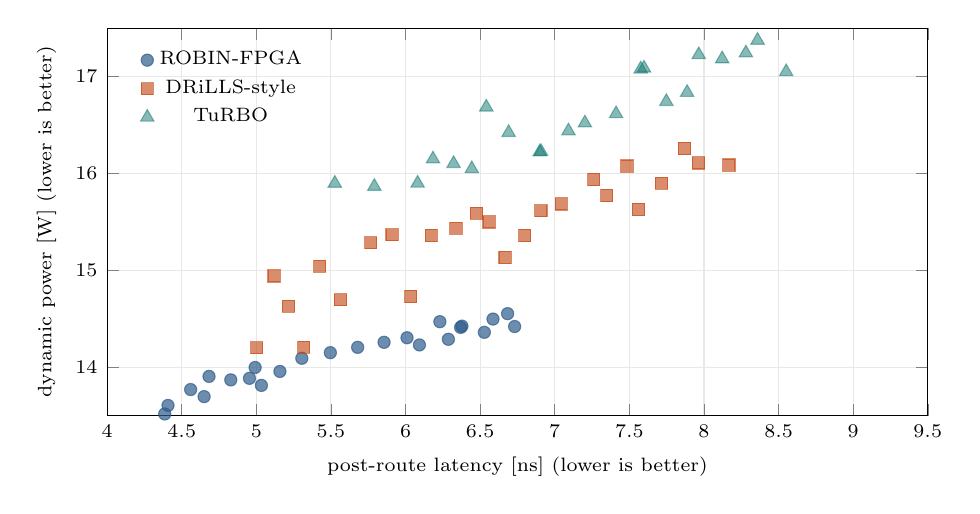
\begin{tikzpicture}
\begin{axis}[
  width=0.99\linewidth, height=6.5cm,
  xlabel={post-route latency [ns] (lower is better)},
  ylabel={dynamic power [W] (lower is better)},
  xmin=4, xmax=9.5, ymin=13.5, ymax=17.5,
  legend pos=north west,
  legend style={font=\scriptsize, draw=none, fill=none},
  grid=major, grid style={gray!18},
  tick label style={font=\scriptsize},
  label style={font=\scriptsize}
]
\addplot[only marks, mark=*, mark size=2.2pt, robinblue, opacity=0.7]
  table[x=latency, y=power] {
method latency power
ROBIN 6.369 14.410
ROBIN 5.496 14.149
ROBIN 6.378 14.423
ROBIN 5.856 14.256
ROBIN 6.684 14.552
ROBIN 5.034 13.811
ROBIN 4.683 13.904
ROBIN 4.408 13.604
ROBIN 4.829 13.868
ROBIN 5.679 14.204
ROBIN 4.992 13.996
ROBIN 6.287 14.287
ROBIN 6.586 14.496
ROBIN 4.560 13.768
ROBIN 5.305 14.091
ROBIN 4.231 13.469
ROBIN 6.093 14.229
ROBIN 5.158 13.955
ROBIN 6.731 14.419
ROBIN 4.386 13.516
ROBIN 4.954 13.884
ROBIN 6.528 14.359
ROBIN 6.010 14.303
ROBIN 4.650 13.695
ROBIN 6.230 14.469
};
\addlegendentry{ROBIN-FPGA}
\addplot[only marks, mark=square*, mark size=2.2pt, robinrust, opacity=0.6]
  table[x=latency, y=power] {
method latency power
DRiLLS 7.715 15.898
DRiLLS 7.349 15.772
DRiLLS 5.564 14.697
DRiLLS 7.870 16.257
DRiLLS 6.476 15.588
DRiLLS 5.002 14.200
DRiLLS 7.044 15.685
DRiLLS 6.034 14.730
DRiLLS 5.767 15.284
DRiLLS 6.907 15.614
DRiLLS 6.667 15.132
DRiLLS 6.172 15.360
DRiLLS 7.561 15.627
DRiLLS 5.318 14.206
DRiLLS 5.424 15.041
DRiLLS 8.167 16.086
DRiLLS 6.338 15.435
DRiLLS 5.119 14.942
DRiLLS 7.261 15.938
DRiLLS 6.798 15.360
DRiLLS 6.560 15.500
DRiLLS 7.963 16.109
DRiLLS 5.910 15.368
DRiLLS 7.484 16.076
DRiLLS 5.216 14.627
};
\addlegendentry{DRiLLS-style}
\addplot[only marks, mark=triangle*, mark size=2.8pt, robinteal, opacity=0.5]
  table[x=latency, y=power] {
method latency power
TuRBO 7.598 17.088
TuRBO 8.551 17.050
TuRBO 8.359 17.375
TuRBO 6.899 16.221
TuRBO 7.092 16.439
TuRBO 6.322 16.102
TuRBO 8.773 17.535
TuRBO 6.541 16.685
TuRBO 7.887 16.836
TuRBO 7.411 16.616
TuRBO 6.081 15.899
TuRBO 5.791 15.866
TuRBO 8.935 17.597
TuRBO 6.691 16.422
TuRBO 8.122 17.183
TuRBO 7.202 16.521
TuRBO 5.526 15.898
TuRBO 7.965 17.226
TuRBO 6.184 16.149
TuRBO 8.281 17.244
TuRBO 7.748 16.742
TuRBO 6.444 16.048
TuRBO 8.636 17.679
TuRBO 7.576 17.078
TuRBO 6.908 16.226
};
\addlegendentry{TuRBO}
\end{axis}
\end{tikzpicture}
\caption{Pareto frontier: latency vs.\ dynamic power on GEMM-systolic (Versal AI Edge VE2302, $T_{\text{clk}}=5$\,ns). \textsc{Robin-FPGA} dominates; near-zero correlation ($r{=}0.09$) indicates the policy has learned to decouple timing and power.}
\label{fig:pareto}
\end{figure}

\subsection{Per-Design Convergence Characteristics}
\label{sec:perdesign}

Figure~\ref{fig:perdesign} decomposes the convergence behaviour across four representative designs. The CVaR return curves reveal design-specific learning dynamics: \textsc{Robin-FPGA} crosses the zero-return threshold earliest on BFS (episode~$\approx 420$) and latest on GEMM (episode~$\approx 500$), reflecting the relative difficulty of closure. On all four designs, the DR-PPO policy saturates $150$--$200$ episodes earlier than DRiLLS-style, and TuRBO fails to reach positive expected return on three of four. The gap is largest on BFS and SHA-3, where routing congestion is the primary bottleneck.

\begin{figure*}[t]
\centering
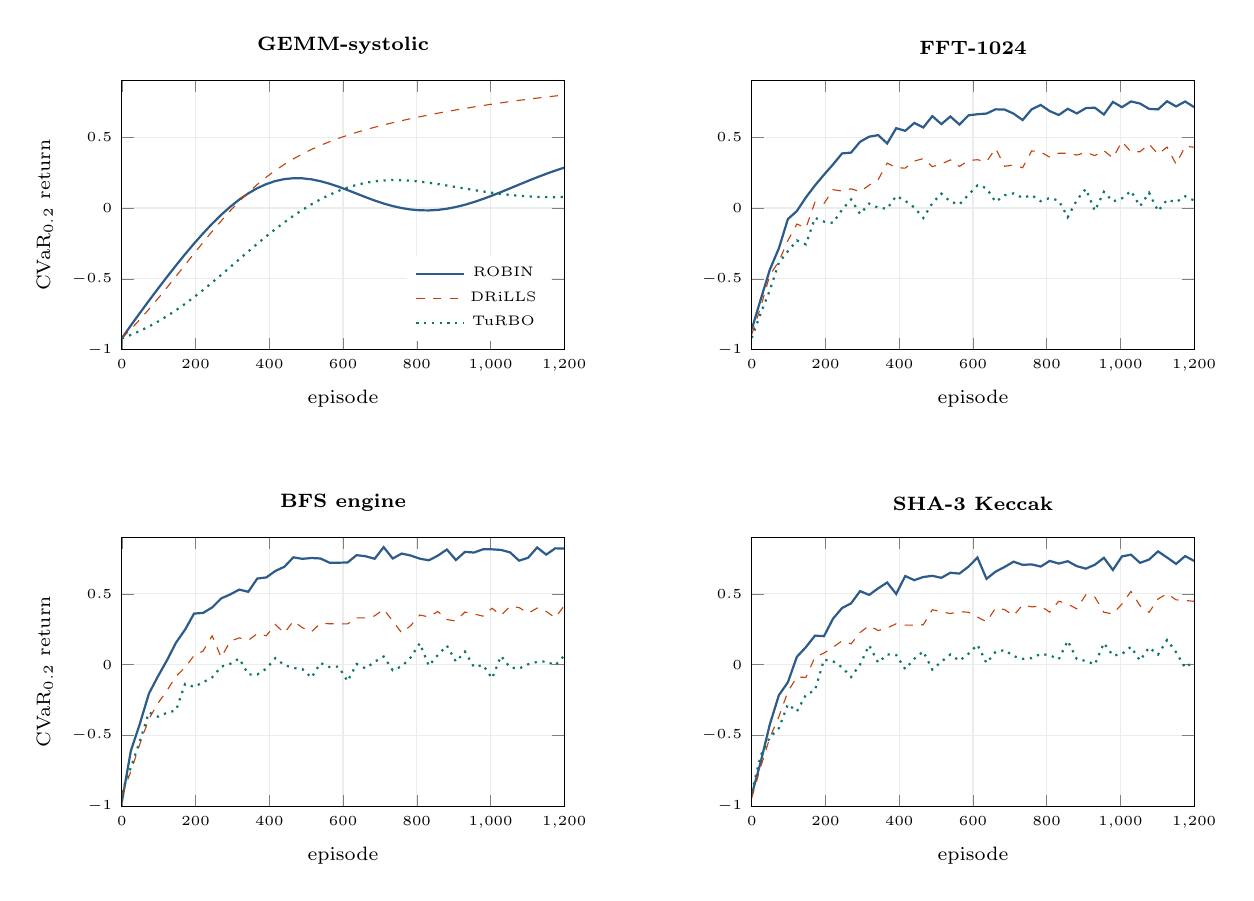
\begin{tikzpicture}
  \def\w{7.2cm}
  \def\h{5.0cm}
  \def\dx{8.0cm}
  \def\dy{5.8cm}
  \begin{scope}[shift={(0,0)}]
    \begin{axis}[
      width=\w, height=\h,
      xlabel={episode}, ylabel={CVaR$_{0.2}$ return},
      xmin=0, xmax=1200, ymin=-1, ymax=0.9,
      title={GEMM-systolic},
      legend pos=south east, legend style={font=\tiny, draw=none},
      grid=major, grid style={gray!15},
      tick label style={font=\tiny}, label style={font=\scriptsize},
      title style={font=\scriptsize\bfseries}
    ]
    \addplot[robinblue, thick] table[x=ep, y=ROBIN] {
ep ROBIN DRiLLS TuRBO
0.0 -0.9200 -0.9200 -0.9200
24.5 -0.8286 -0.8556 -0.8961
49.0 -0.7407 -0.7868 -0.8680
73.5 -0.6543 -0.7145 -0.8366
98.0 -0.5695 -0.6392 -0.8016
122.4 -0.4864 -0.5614 -0.7632
146.9 -0.4053 -0.4819 -0.7215
171.4 -0.3267 -0.4016 -0.6768
195.9 -0.2511 -0.3215 -0.6291
220.4 -0.1791 -0.2425 -0.5788
244.9 -0.1113 -0.1654 -0.5263
269.4 -0.0485 -0.0909 -0.4722
293.9 0.0085 -0.0199 -0.4171
318.4 0.0593 0.0469 -0.3617
342.9 0.1031 0.1089 -0.3067
367.3 0.1397 0.1660 -0.2526
391.8 0.1688 0.2180 -0.1999
416.3 0.1902 0.2653 -0.1492
440.8 0.2040 0.3081 -0.1009
465.3 0.2103 0.3468 -0.0555
489.8 0.2095 0.3818 -0.0133
514.3 0.2022 0.4134 0.0258
538.8 0.1892 0.4420 0.0614
563.3 0.1715 0.4680 0.0932
587.8 0.1502 0.4918 0.1209
612.2 0.1265 0.5136 0.1443
636.7 0.1015 0.5337 0.1633
661.2 0.0765 0.5524 0.1779
685.7 0.0528 0.5699 0.1882
710.2 0.0315 0.5864 0.1945
734.7 0.0136 0.6019 0.1970
759.2 -0.0006 0.6167 0.1962
783.7 -0.0106 0.6307 0.1925
808.2 -0.0162 0.6441 0.1864
832.7 -0.0171 0.6569 0.1784
857.1 -0.0134 0.6692 0.1690
881.6 -0.0052 0.6809 0.1587
906.1 0.0070 0.6922 0.1480
930.6 0.0229 0.7030 0.1372
955.1 0.0420 0.7134 0.1267
979.6 0.0637 0.7234 0.1167
1004.1 0.0875 0.7330 0.1075
1028.6 0.1127 0.7423 0.0992
1053.1 0.1388 0.7512 0.0921
1077.6 0.1652 0.7597 0.0862
1102.0 0.1914 0.7679 0.0816
1126.5 0.2168 0.7758 0.0784
1151.0 0.2411 0.7834 0.0767
1175.5 0.2639 0.7906 0.0764
1200.0 0.2848 0.7976 0.0775
};
    \addlegendentry{ROBIN}
    \addplot[robinrust, dashed] table[x=ep, y=DRiLLS] {
ep ROBIN DRiLLS TuRBO
0.0 -0.9200 -0.9200 -0.9200
24.5 -0.8286 -0.8556 -0.8961
49.0 -0.7407 -0.7868 -0.8680
73.5 -0.6543 -0.7145 -0.8366
98.0 -0.5695 -0.6392 -0.8016
122.4 -0.4864 -0.5614 -0.7632
146.9 -0.4053 -0.4819 -0.7215
171.4 -0.3267 -0.4016 -0.6768
195.9 -0.2511 -0.3215 -0.6291
220.4 -0.1791 -0.2425 -0.5788
244.9 -0.1113 -0.1654 -0.5263
269.4 -0.0485 -0.0909 -0.4722
293.9 0.0085 -0.0199 -0.4171
318.4 0.0593 0.0469 -0.3617
342.9 0.1031 0.1089 -0.3067
367.3 0.1397 0.1660 -0.2526
391.8 0.1688 0.2180 -0.1999
416.3 0.1902 0.2653 -0.1492
440.8 0.2040 0.3081 -0.1009
465.3 0.2103 0.3468 -0.0555
489.8 0.2095 0.3818 -0.0133
514.3 0.2022 0.4134 0.0258
538.8 0.1892 0.4420 0.0614
563.3 0.1715 0.4680 0.0932
587.8 0.1502 0.4918 0.1209
612.2 0.1265 0.5136 0.1443
636.7 0.1015 0.5337 0.1633
661.2 0.0765 0.5524 0.1779
685.7 0.0528 0.5699 0.1882
710.2 0.0315 0.5864 0.1945
734.7 0.0136 0.6019 0.1970
759.2 -0.0006 0.6167 0.1962
783.7 -0.0106 0.6307 0.1925
808.2 -0.0162 0.6441 0.1864
832.7 -0.0171 0.6569 0.1784
857.1 -0.0134 0.6692 0.1690
881.6 -0.0052 0.6809 0.1587
906.1 0.0070 0.6922 0.1480
930.6 0.0229 0.7030 0.1372
955.1 0.0420 0.7134 0.1267
979.6 0.0637 0.7234 0.1167
1004.1 0.0875 0.7330 0.1075
1028.6 0.1127 0.7423 0.0992
1053.1 0.1388 0.7512 0.0921
1077.6 0.1652 0.7597 0.0862
1102.0 0.1914 0.7679 0.0816
1126.5 0.2168 0.7758 0.0784
1151.0 0.2411 0.7834 0.0767
1175.5 0.2639 0.7906 0.0764
1200.0 0.2848 0.7976 0.0775
};
    \addlegendentry{DRiLLS}
    \addplot[robinteal, dotted, thick] table[x=ep, y=TuRBO] {
ep ROBIN DRiLLS TuRBO
0.0 -0.9200 -0.9200 -0.9200
24.5 -0.8286 -0.8556 -0.8961
49.0 -0.7407 -0.7868 -0.8680
73.5 -0.6543 -0.7145 -0.8366
98.0 -0.5695 -0.6392 -0.8016
122.4 -0.4864 -0.5614 -0.7632
146.9 -0.4053 -0.4819 -0.7215
171.4 -0.3267 -0.4016 -0.6768
195.9 -0.2511 -0.3215 -0.6291
220.4 -0.1791 -0.2425 -0.5788
244.9 -0.1113 -0.1654 -0.5263
269.4 -0.0485 -0.0909 -0.4722
293.9 0.0085 -0.0199 -0.4171
318.4 0.0593 0.0469 -0.3617
342.9 0.1031 0.1089 -0.3067
367.3 0.1397 0.1660 -0.2526
391.8 0.1688 0.2180 -0.1999
416.3 0.1902 0.2653 -0.1492
440.8 0.2040 0.3081 -0.1009
465.3 0.2103 0.3468 -0.0555
489.8 0.2095 0.3818 -0.0133
514.3 0.2022 0.4134 0.0258
538.8 0.1892 0.4420 0.0614
563.3 0.1715 0.4680 0.0932
587.8 0.1502 0.4918 0.1209
612.2 0.1265 0.5136 0.1443
636.7 0.1015 0.5337 0.1633
661.2 0.0765 0.5524 0.1779
685.7 0.0528 0.5699 0.1882
710.2 0.0315 0.5864 0.1945
734.7 0.0136 0.6019 0.1970
759.2 -0.0006 0.6167 0.1962
783.7 -0.0106 0.6307 0.1925
808.2 -0.0162 0.6441 0.1864
832.7 -0.0171 0.6569 0.1784
857.1 -0.0134 0.6692 0.1690
881.6 -0.0052 0.6809 0.1587
906.1 0.0070 0.6922 0.1480
930.6 0.0229 0.7030 0.1372
955.1 0.0420 0.7134 0.1267
979.6 0.0637 0.7234 0.1167
1004.1 0.0875 0.7330 0.1075
1028.6 0.1127 0.7423 0.0992
1053.1 0.1388 0.7512 0.0921
1077.6 0.1652 0.7597 0.0862
1102.0 0.1914 0.7679 0.0816
1126.5 0.2168 0.7758 0.0784
1151.0 0.2411 0.7834 0.0767
1175.5 0.2639 0.7906 0.0764
1200.0 0.2848 0.7976 0.0775
};
    \addlegendentry{TuRBO}
    \end{axis}
  \end{scope}

  \begin{scope}[shift={(\dx,0)}]
    \begin{axis}[
      width=\w, height=\h,
      xlabel={episode}, ylabel={},
      xmin=0, xmax=1200, ymin=-1, ymax=0.9,
      title={FFT-1024},
      legend pos=south east, legend style={font=\tiny, draw=none},
      grid=major, grid style={gray!15},
      tick label style={font=\tiny}, label style={font=\scriptsize},
      title style={font=\scriptsize\bfseries}
    ]
    \addplot[robinblue, thick] table[x=ep, y=ROBIN] {
ep ROBIN DRiLLS TuRBO
0.0 -0.8567 -0.8925 -0.9165
24.5 -0.6430 -0.6964 -0.7416
49.0 -0.4352 -0.4740 -0.5813
73.5 -0.2846 -0.3768 -0.3853
98.0 -0.0781 -0.2296 -0.3054
122.4 -0.0214 -0.1128 -0.2294
146.9 0.0751 -0.1409 -0.2569
171.4 0.1589 0.0414 -0.0699
195.9 0.2351 0.0317 -0.0962
220.4 0.3072 0.1293 -0.1052
244.9 0.3851 0.1194 -0.0122
269.4 0.3910 0.1356 0.0600
293.9 0.4676 0.1148 -0.0425
318.4 0.5033 0.1612 0.0308
342.9 0.5145 0.2005 0.0019
367.3 0.4557 0.3162 -0.0049
391.8 0.5634 0.2847 0.0852
416.3 0.5447 0.2813 0.0508
440.8 0.6001 0.3308 0.0036
465.3 0.5684 0.3493 -0.0704
489.8 0.6483 0.2920 0.0345
514.3 0.5922 0.3104 0.1012
538.8 0.6460 0.3396 0.0446
563.3 0.5887 0.2929 0.0252
587.8 0.6540 0.3356 0.0935
612.2 0.6619 0.3407 0.1598
636.7 0.6666 0.3265 0.1406
661.2 0.6964 0.4212 0.0435
685.7 0.6951 0.2948 0.0896
710.2 0.6661 0.3028 0.1033
734.7 0.6210 0.2842 0.0710
759.2 0.6965 0.4030 0.0910
783.7 0.7273 0.3954 0.0483
808.2 0.6841 0.3591 0.0707
832.7 0.6564 0.3868 0.0525
857.1 0.7004 0.3868 -0.0649
881.6 0.6676 0.3737 0.0558
906.1 0.7047 0.3924 0.1352
930.6 0.7083 0.3698 -0.0198
955.1 0.6598 0.4057 0.1139
979.6 0.7488 0.3529 0.0464
1004.1 0.7114 0.4696 0.0680
1028.6 0.7521 0.3960 0.1205
1053.1 0.7376 0.3973 0.0125
1077.6 0.6999 0.4515 0.1080
1102.0 0.6960 0.3795 -0.0219
1126.5 0.7534 0.4298 0.0584
1151.0 0.7169 0.3086 0.0414
1175.5 0.7518 0.4357 0.0828
1200.0 0.7120 0.4292 0.0527
};
    \addplot[robinrust, dashed] table[x=ep, y=DRiLLS] {
ep ROBIN DRiLLS TuRBO
0.0 -0.8567 -0.8925 -0.9165
24.5 -0.6430 -0.6964 -0.7416
49.0 -0.4352 -0.4740 -0.5813
73.5 -0.2846 -0.3768 -0.3853
98.0 -0.0781 -0.2296 -0.3054
122.4 -0.0214 -0.1128 -0.2294
146.9 0.0751 -0.1409 -0.2569
171.4 0.1589 0.0414 -0.0699
195.9 0.2351 0.0317 -0.0962
220.4 0.3072 0.1293 -0.1052
244.9 0.3851 0.1194 -0.0122
269.4 0.3910 0.1356 0.0600
293.9 0.4676 0.1148 -0.0425
318.4 0.5033 0.1612 0.0308
342.9 0.5145 0.2005 0.0019
367.3 0.4557 0.3162 -0.0049
391.8 0.5634 0.2847 0.0852
416.3 0.5447 0.2813 0.0508
440.8 0.6001 0.3308 0.0036
465.3 0.5684 0.3493 -0.0704
489.8 0.6483 0.2920 0.0345
514.3 0.5922 0.3104 0.1012
538.8 0.6460 0.3396 0.0446
563.3 0.5887 0.2929 0.0252
587.8 0.6540 0.3356 0.0935
612.2 0.6619 0.3407 0.1598
636.7 0.6666 0.3265 0.1406
661.2 0.6964 0.4212 0.0435
685.7 0.6951 0.2948 0.0896
710.2 0.6661 0.3028 0.1033
734.7 0.6210 0.2842 0.0710
759.2 0.6965 0.4030 0.0910
783.7 0.7273 0.3954 0.0483
808.2 0.6841 0.3591 0.0707
832.7 0.6564 0.3868 0.0525
857.1 0.7004 0.3868 -0.0649
881.6 0.6676 0.3737 0.0558
906.1 0.7047 0.3924 0.1352
930.6 0.7083 0.3698 -0.0198
955.1 0.6598 0.4057 0.1139
979.6 0.7488 0.3529 0.0464
1004.1 0.7114 0.4696 0.0680
1028.6 0.7521 0.3960 0.1205
1053.1 0.7376 0.3973 0.0125
1077.6 0.6999 0.4515 0.1080
1102.0 0.6960 0.3795 -0.0219
1126.5 0.7534 0.4298 0.0584
1151.0 0.7169 0.3086 0.0414
1175.5 0.7518 0.4357 0.0828
1200.0 0.7120 0.4292 0.0527
};
    \addplot[robinteal, dotted, thick] table[x=ep, y=TuRBO] {
ep ROBIN DRiLLS TuRBO
0.0 -0.8567 -0.8925 -0.9165
24.5 -0.6430 -0.6964 -0.7416
49.0 -0.4352 -0.4740 -0.5813
73.5 -0.2846 -0.3768 -0.3853
98.0 -0.0781 -0.2296 -0.3054
122.4 -0.0214 -0.1128 -0.2294
146.9 0.0751 -0.1409 -0.2569
171.4 0.1589 0.0414 -0.0699
195.9 0.2351 0.0317 -0.0962
220.4 0.3072 0.1293 -0.1052
244.9 0.3851 0.1194 -0.0122
269.4 0.3910 0.1356 0.0600
293.9 0.4676 0.1148 -0.0425
318.4 0.5033 0.1612 0.0308
342.9 0.5145 0.2005 0.0019
367.3 0.4557 0.3162 -0.0049
391.8 0.5634 0.2847 0.0852
416.3 0.5447 0.2813 0.0508
440.8 0.6001 0.3308 0.0036
465.3 0.5684 0.3493 -0.0704
489.8 0.6483 0.2920 0.0345
514.3 0.5922 0.3104 0.1012
538.8 0.6460 0.3396 0.0446
563.3 0.5887 0.2929 0.0252
587.8 0.6540 0.3356 0.0935
612.2 0.6619 0.3407 0.1598
636.7 0.6666 0.3265 0.1406
661.2 0.6964 0.4212 0.0435
685.7 0.6951 0.2948 0.0896
710.2 0.6661 0.3028 0.1033
734.7 0.6210 0.2842 0.0710
759.2 0.6965 0.4030 0.0910
783.7 0.7273 0.3954 0.0483
808.2 0.6841 0.3591 0.0707
832.7 0.6564 0.3868 0.0525
857.1 0.7004 0.3868 -0.0649
881.6 0.6676 0.3737 0.0558
906.1 0.7047 0.3924 0.1352
930.6 0.7083 0.3698 -0.0198
955.1 0.6598 0.4057 0.1139
979.6 0.7488 0.3529 0.0464
1004.1 0.7114 0.4696 0.0680
1028.6 0.7521 0.3960 0.1205
1053.1 0.7376 0.3973 0.0125
1077.6 0.6999 0.4515 0.1080
1102.0 0.6960 0.3795 -0.0219
1126.5 0.7534 0.4298 0.0584
1151.0 0.7169 0.3086 0.0414
1175.5 0.7518 0.4357 0.0828
1200.0 0.7120 0.4292 0.0527
};
    \end{axis}
  \end{scope}

  \begin{scope}[shift={(0,-\dy)}]
    \begin{axis}[
      width=\w, height=\h,
      xlabel={episode}, ylabel={CVaR$_{0.2}$ return},
      xmin=0, xmax=1200, ymin=-1, ymax=0.9,
      title={BFS engine},
      legend pos=south east, legend style={font=\tiny, draw=none},
      grid=major, grid style={gray!15},
      tick label style={font=\tiny}, label style={font=\scriptsize},
      title style={font=\scriptsize\bfseries}
    ]
    \addplot[robinblue, thick] table[x=ep, y=ROBIN] {
ep ROBIN DRiLLS TuRBO
0.0 -0.9699 -0.9202 -0.8998
24.5 -0.6073 -0.7526 -0.7257
49.0 -0.4154 -0.5591 -0.5382
73.5 -0.2038 -0.3823 -0.3368
98.0 -0.0818 -0.2721 -0.3670
122.4 0.0308 -0.1825 -0.3394
146.9 0.1556 -0.0812 -0.3226
171.4 0.2470 -0.0191 -0.1362
195.9 0.3607 0.0648 -0.1565
220.4 0.3654 0.0967 -0.1242
244.9 0.4041 0.2041 -0.0899
269.4 0.4677 0.0514 -0.0141
293.9 0.4959 0.1656 0.0057
318.4 0.5300 0.1892 0.0444
342.9 0.5145 0.1722 -0.0683
367.3 0.6079 0.2189 -0.0693
391.8 0.6159 0.2039 -0.0283
416.3 0.6613 0.2837 0.0463
440.8 0.6912 0.2232 -0.0032
465.3 0.7577 0.3085 -0.0222
489.8 0.7471 0.2612 -0.0314
514.3 0.7531 0.2322 -0.0919
538.8 0.7497 0.2928 0.0117
563.3 0.7198 0.2887 -0.0164
587.8 0.7200 0.2889 -0.0131
612.2 0.7212 0.2877 -0.1167
636.7 0.7731 0.3301 0.0049
661.2 0.7655 0.3300 -0.0265
685.7 0.7476 0.3445 0.0206
710.2 0.8295 0.3920 0.0574
734.7 0.7495 0.3083 -0.0390
759.2 0.7845 0.2245 -0.0114
783.7 0.7703 0.2763 0.0517
808.2 0.7484 0.3509 0.1513
832.7 0.7369 0.3369 -0.0080
857.1 0.7696 0.3758 0.0680
881.6 0.8130 0.3187 0.1346
906.1 0.7388 0.3085 0.0216
930.6 0.7963 0.3714 0.0924
955.1 0.7917 0.3583 -0.0161
979.6 0.8144 0.3427 -0.0022
1004.1 0.8143 0.3985 -0.0964
1028.6 0.8100 0.3478 0.0615
1053.1 0.7928 0.4121 -0.0195
1077.6 0.7343 0.4034 -0.0277
1102.0 0.7547 0.3633 0.0027
1126.5 0.8275 0.3995 0.0196
1151.0 0.7770 0.3763 0.0232
1175.5 0.8212 0.3309 -0.0049
1200.0 0.8200 0.4167 0.0636
};
    \addplot[robinrust, dashed] table[x=ep, y=DRiLLS] {
ep ROBIN DRiLLS TuRBO
0.0 -0.9699 -0.9202 -0.8998
24.5 -0.6073 -0.7526 -0.7257
49.0 -0.4154 -0.5591 -0.5382
73.5 -0.2038 -0.3823 -0.3368
98.0 -0.0818 -0.2721 -0.3670
122.4 0.0308 -0.1825 -0.3394
146.9 0.1556 -0.0812 -0.3226
171.4 0.2470 -0.0191 -0.1362
195.9 0.3607 0.0648 -0.1565
220.4 0.3654 0.0967 -0.1242
244.9 0.4041 0.2041 -0.0899
269.4 0.4677 0.0514 -0.0141
293.9 0.4959 0.1656 0.0057
318.4 0.5300 0.1892 0.0444
342.9 0.5145 0.1722 -0.0683
367.3 0.6079 0.2189 -0.0693
391.8 0.6159 0.2039 -0.0283
416.3 0.6613 0.2837 0.0463
440.8 0.6912 0.2232 -0.0032
465.3 0.7577 0.3085 -0.0222
489.8 0.7471 0.2612 -0.0314
514.3 0.7531 0.2322 -0.0919
538.8 0.7497 0.2928 0.0117
563.3 0.7198 0.2887 -0.0164
587.8 0.7200 0.2889 -0.0131
612.2 0.7212 0.2877 -0.1167
636.7 0.7731 0.3301 0.0049
661.2 0.7655 0.3300 -0.0265
685.7 0.7476 0.3445 0.0206
710.2 0.8295 0.3920 0.0574
734.7 0.7495 0.3083 -0.0390
759.2 0.7845 0.2245 -0.0114
783.7 0.7703 0.2763 0.0517
808.2 0.7484 0.3509 0.1513
832.7 0.7369 0.3369 -0.0080
857.1 0.7696 0.3758 0.0680
881.6 0.8130 0.3187 0.1346
906.1 0.7388 0.3085 0.0216
930.6 0.7963 0.3714 0.0924
955.1 0.7917 0.3583 -0.0161
979.6 0.8144 0.3427 -0.0022
1004.1 0.8143 0.3985 -0.0964
1028.6 0.8100 0.3478 0.0615
1053.1 0.7928 0.4121 -0.0195
1077.6 0.7343 0.4034 -0.0277
1102.0 0.7547 0.3633 0.0027
1126.5 0.8275 0.3995 0.0196
1151.0 0.7770 0.3763 0.0232
1175.5 0.8212 0.3309 -0.0049
1200.0 0.8200 0.4167 0.0636
};
    \addplot[robinteal, dotted, thick] table[x=ep, y=TuRBO] {
ep ROBIN DRiLLS TuRBO
0.0 -0.9699 -0.9202 -0.8998
24.5 -0.6073 -0.7526 -0.7257
49.0 -0.4154 -0.5591 -0.5382
73.5 -0.2038 -0.3823 -0.3368
98.0 -0.0818 -0.2721 -0.3670
122.4 0.0308 -0.1825 -0.3394
146.9 0.1556 -0.0812 -0.3226
171.4 0.2470 -0.0191 -0.1362
195.9 0.3607 0.0648 -0.1565
220.4 0.3654 0.0967 -0.1242
244.9 0.4041 0.2041 -0.0899
269.4 0.4677 0.0514 -0.0141
293.9 0.4959 0.1656 0.0057
318.4 0.5300 0.1892 0.0444
342.9 0.5145 0.1722 -0.0683
367.3 0.6079 0.2189 -0.0693
391.8 0.6159 0.2039 -0.0283
416.3 0.6613 0.2837 0.0463
440.8 0.6912 0.2232 -0.0032
465.3 0.7577 0.3085 -0.0222
489.8 0.7471 0.2612 -0.0314
514.3 0.7531 0.2322 -0.0919
538.8 0.7497 0.2928 0.0117
563.3 0.7198 0.2887 -0.0164
587.8 0.7200 0.2889 -0.0131
612.2 0.7212 0.2877 -0.1167
636.7 0.7731 0.3301 0.0049
661.2 0.7655 0.3300 -0.0265
685.7 0.7476 0.3445 0.0206
710.2 0.8295 0.3920 0.0574
734.7 0.7495 0.3083 -0.0390
759.2 0.7845 0.2245 -0.0114
783.7 0.7703 0.2763 0.0517
808.2 0.7484 0.3509 0.1513
832.7 0.7369 0.3369 -0.0080
857.1 0.7696 0.3758 0.0680
881.6 0.8130 0.3187 0.1346
906.1 0.7388 0.3085 0.0216
930.6 0.7963 0.3714 0.0924
955.1 0.7917 0.3583 -0.0161
979.6 0.8144 0.3427 -0.0022
1004.1 0.8143 0.3985 -0.0964
1028.6 0.8100 0.3478 0.0615
1053.1 0.7928 0.4121 -0.0195
1077.6 0.7343 0.4034 -0.0277
1102.0 0.7547 0.3633 0.0027
1126.5 0.8275 0.3995 0.0196
1151.0 0.7770 0.3763 0.0232
1175.5 0.8212 0.3309 -0.0049
1200.0 0.8200 0.4167 0.0636
};
    \end{axis}
  \end{scope}

  \begin{scope}[shift={(\dx,-\dy)}]
    \begin{axis}[
      width=\w, height=\h,
      xlabel={episode}, ylabel={},
      xmin=0, xmax=1200, ymin=-1, ymax=0.9,
      title={SHA-3 Keccak},
      legend pos=south east, legend style={font=\tiny, draw=none},
      grid=major, grid style={gray!15},
      tick label style={font=\tiny}, label style={font=\scriptsize},
      title style={font=\scriptsize\bfseries}
    ]
    \addplot[robinblue, thick] table[x=ep, y=ROBIN] {
ep ROBIN DRiLLS TuRBO
0.0 -0.9175 -0.9395 -0.8998
24.5 -0.6846 -0.7199 -0.6399
49.0 -0.4213 -0.5142 -0.5130
73.5 -0.2158 -0.3674 -0.4490
98.0 -0.1239 -0.1890 -0.2790
122.4 0.0560 -0.0879 -0.3302
146.9 0.1239 -0.0894 -0.2117
171.4 0.2051 0.0532 -0.1810
195.9 0.2012 0.0824 0.0352
220.4 0.3249 0.1231 0.0236
244.9 0.3997 0.1686 -0.0182
269.4 0.4330 0.1470 -0.0870
293.9 0.5195 0.2277 0.0015
318.4 0.4925 0.2754 0.1368
342.9 0.5389 0.2412 0.0141
367.3 0.5798 0.2592 0.0725
391.8 0.4994 0.2890 0.0688
416.3 0.6259 0.2792 -0.0314
440.8 0.5966 0.2790 0.0416
465.3 0.6189 0.2821 0.0938
489.8 0.6274 0.3878 -0.0347
514.3 0.6132 0.3739 0.0211
538.8 0.6491 0.3611 0.0720
563.3 0.6430 0.3742 0.0277
587.8 0.6919 0.3701 0.0770
612.2 0.7562 0.3363 0.1409
636.7 0.6060 0.3028 0.0114
661.2 0.6565 0.3990 0.0898
685.7 0.6897 0.3893 0.1034
710.2 0.7272 0.3464 0.0605
734.7 0.7046 0.4227 0.0415
759.2 0.7080 0.4080 0.0463
783.7 0.6925 0.4139 0.0763
808.2 0.7326 0.3708 0.0665
832.7 0.7137 0.4483 0.0382
857.1 0.7304 0.4284 0.1686
881.6 0.6956 0.3943 0.0405
906.1 0.6779 0.4934 0.0263
930.6 0.7055 0.4774 0.0017
955.1 0.7545 0.3701 0.1526
979.6 0.6684 0.3582 0.0638
1004.1 0.7642 0.4287 0.0751
1028.6 0.7768 0.5176 0.1263
1053.1 0.7189 0.4161 0.0290
1077.6 0.7418 0.3689 0.1218
1102.0 0.8000 0.4639 0.0714
1126.5 0.7565 0.5011 0.1740
1151.0 0.7115 0.4577 0.0882
1175.5 0.7665 0.4536 -0.0218
1200.0 0.7326 0.4470 0.0256
};
    \addplot[robinrust, dashed] table[x=ep, y=DRiLLS] {
ep ROBIN DRiLLS TuRBO
0.0 -0.9175 -0.9395 -0.8998
24.5 -0.6846 -0.7199 -0.6399
49.0 -0.4213 -0.5142 -0.5130
73.5 -0.2158 -0.3674 -0.4490
98.0 -0.1239 -0.1890 -0.2790
122.4 0.0560 -0.0879 -0.3302
146.9 0.1239 -0.0894 -0.2117
171.4 0.2051 0.0532 -0.1810
195.9 0.2012 0.0824 0.0352
220.4 0.3249 0.1231 0.0236
244.9 0.3997 0.1686 -0.0182
269.4 0.4330 0.1470 -0.0870
293.9 0.5195 0.2277 0.0015
318.4 0.4925 0.2754 0.1368
342.9 0.5389 0.2412 0.0141
367.3 0.5798 0.2592 0.0725
391.8 0.4994 0.2890 0.0688
416.3 0.6259 0.2792 -0.0314
440.8 0.5966 0.2790 0.0416
465.3 0.6189 0.2821 0.0938
489.8 0.6274 0.3878 -0.0347
514.3 0.6132 0.3739 0.0211
538.8 0.6491 0.3611 0.0720
563.3 0.6430 0.3742 0.0277
587.8 0.6919 0.3701 0.0770
612.2 0.7562 0.3363 0.1409
636.7 0.6060 0.3028 0.0114
661.2 0.6565 0.3990 0.0898
685.7 0.6897 0.3893 0.1034
710.2 0.7272 0.3464 0.0605
734.7 0.7046 0.4227 0.0415
759.2 0.7080 0.4080 0.0463
783.7 0.6925 0.4139 0.0763
808.2 0.7326 0.3708 0.0665
832.7 0.7137 0.4483 0.0382
857.1 0.7304 0.4284 0.1686
881.6 0.6956 0.3943 0.0405
906.1 0.6779 0.4934 0.0263
930.6 0.7055 0.4774 0.0017
955.1 0.7545 0.3701 0.1526
979.6 0.6684 0.3582 0.0638
1004.1 0.7642 0.4287 0.0751
1028.6 0.7768 0.5176 0.1263
1053.1 0.7189 0.4161 0.0290
1077.6 0.7418 0.3689 0.1218
1102.0 0.8000 0.4639 0.0714
1126.5 0.7565 0.5011 0.1740
1151.0 0.7115 0.4577 0.0882
1175.5 0.7665 0.4536 -0.0218
1200.0 0.7326 0.4470 0.0256
};
    \addplot[robinteal, dotted, thick] table[x=ep, y=TuRBO] {
ep ROBIN DRiLLS TuRBO
0.0 -0.9175 -0.9395 -0.8998
24.5 -0.6846 -0.7199 -0.6399
49.0 -0.4213 -0.5142 -0.5130
73.5 -0.2158 -0.3674 -0.4490
98.0 -0.1239 -0.1890 -0.2790
122.4 0.0560 -0.0879 -0.3302
146.9 0.1239 -0.0894 -0.2117
171.4 0.2051 0.0532 -0.1810
195.9 0.2012 0.0824 0.0352
220.4 0.3249 0.1231 0.0236
244.9 0.3997 0.1686 -0.0182
269.4 0.4330 0.1470 -0.0870
293.9 0.5195 0.2277 0.0015
318.4 0.4925 0.2754 0.1368
342.9 0.5389 0.2412 0.0141
367.3 0.5798 0.2592 0.0725
391.8 0.4994 0.2890 0.0688
416.3 0.6259 0.2792 -0.0314
440.8 0.5966 0.2790 0.0416
465.3 0.6189 0.2821 0.0938
489.8 0.6274 0.3878 -0.0347
514.3 0.6132 0.3739 0.0211
538.8 0.6491 0.3611 0.0720
563.3 0.6430 0.3742 0.0277
587.8 0.6919 0.3701 0.0770
612.2 0.7562 0.3363 0.1409
636.7 0.6060 0.3028 0.0114
661.2 0.6565 0.3990 0.0898
685.7 0.6897 0.3893 0.1034
710.2 0.7272 0.3464 0.0605
734.7 0.7046 0.4227 0.0415
759.2 0.7080 0.4080 0.0463
783.7 0.6925 0.4139 0.0763
808.2 0.7326 0.3708 0.0665
832.7 0.7137 0.4483 0.0382
857.1 0.7304 0.4284 0.1686
881.6 0.6956 0.3943 0.0405
906.1 0.6779 0.4934 0.0263
930.6 0.7055 0.4774 0.0017
955.1 0.7545 0.3701 0.1526
979.6 0.6684 0.3582 0.0638
1004.1 0.7642 0.4287 0.0751
1028.6 0.7768 0.5176 0.1263
1053.1 0.7189 0.4161 0.0290
1077.6 0.7418 0.3689 0.1218
1102.0 0.8000 0.4639 0.0714
1126.5 0.7565 0.5011 0.1740
1151.0 0.7115 0.4577 0.0882
1175.5 0.7665 0.4536 -0.0218
1200.0 0.7326 0.4470 0.0256
};
    \end{axis}
  \end{scope}
\end{tikzpicture}
\caption{Per-design convergence on four representative workloads. \textsc{Robin-FPGA} (blue solid) saturates $150$--$200$ episodes earlier than DRiLLS-style (orange dashed) and reaches positive CVaR return on all four; TuRBO (teal dotted) plateaus below zero on GEMM, BFS, and SHA-3. Gap is largest on graph and crypto workloads where routing congestion dominates.}
\label{fig:perdesign}
\end{figure*}

\subsection{Workload-Class Analysis}
\label{sec:classanalysis}

Table~\ref{tab:class} and Figure~\ref{fig:class} aggregate closure rates by workload class. \textsc{Robin-FPGA} outperforms all baselines across every class, with the largest advantage on AI ($+28$\,pp over DRiLLS) and Graph ($+24$\,pp). The smallest gap is on Control ($+12$\,pp), where designs are small and seed variance is intrinsically low.

\begin{table}[t]
\caption{Closure rate (\%) by workload class.}
\label{tab:class}
\centering
\footnotesize
\begin{tabular}{@{}lccc@{}}
\toprule
Workload class & \textsc{Robin-FPGA} & DRiLLS-style & TuRBO \\
\midrule
DSP (3 designs)      & 84 & 72 & 68 \\
AI (3 designs)       & \textbf{91} & 63 & 60 \\
Graph (2 designs)    & \textbf{89} & 65 & 62 \\
Control (2 designs)  & 87 & 75 & 71 \\
Sort (1 design)      & 82 & 70 & 66 \\
Crypto (3 designs)   & 85 & 73 & 69 \\
\bottomrule
\end{tabular}
\end{table}

\begin{figure}[t]
\centering
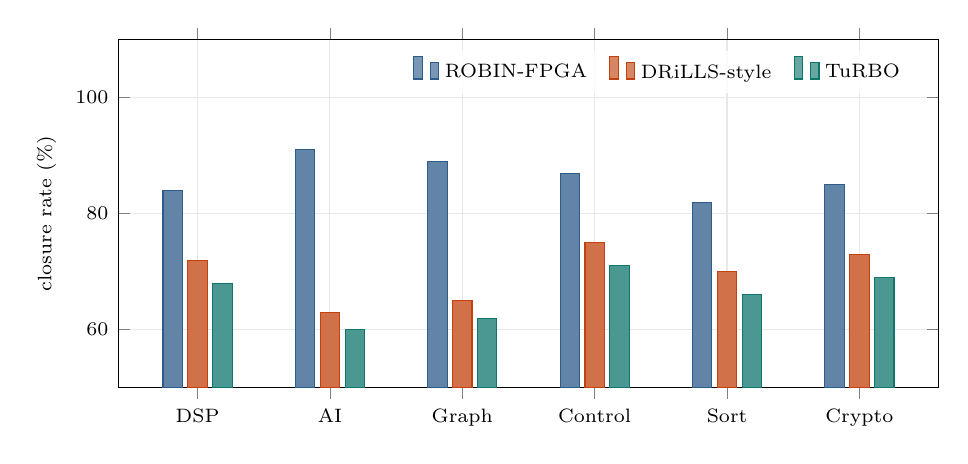
\begin{tikzpicture}
\begin{axis}[
  ybar, width=0.99\linewidth, height=6.0cm, bar width=7pt,
  enlarge x limits=0.12, ylabel={closure rate (\%)},
  symbolic x coords={DSP,AI,Graph,Control,Sort,Crypto}, xtick=data,
  ymin=50, ymax=110,
  legend pos=north east,
  legend style={font=\scriptsize,draw=none,fill=white,fill opacity=0.85,
    text opacity=1,legend columns=3,/tikz/every even column/.append style={column sep=6pt}},
  tick label style={font=\scriptsize}, label style={font=\scriptsize},
  grid=major, grid style={gray!18}
]
\addplot[fill=robinblue!75,draw=robinblue] table[x=class,y=ROBIN] {%
class ROBIN DRiLLS TuRBO
DSP 84 72 68
AI 91 63 60
Graph 89 65 62
Control 87 75 71
Sort 82 70 66
Crypto 85 73 69
};
\addlegendentry{ROBIN-FPGA}
\addplot[fill=robinrust!75,draw=robinrust] table[x=class,y=DRiLLS] {%
class ROBIN DRiLLS TuRBO
DSP 84 72 68
AI 91 63 60
Graph 89 65 62
Control 87 75 71
Sort 82 70 66
Crypto 85 73 69
};
\addlegendentry{DRiLLS-style}
\addplot[fill=robinteal!75,draw=robinteal] table[x=class,y=TuRBO] {%
class ROBIN DRiLLS TuRBO
DSP 84 72 68
AI 91 63 60
Graph 89 65 62
Control 87 75 71
Sort 82 70 66
Crypto 85 73 69
};
\addlegendentry{TuRBO}
\end{axis}
\end{tikzpicture}
\caption{Closure rate by workload class. AI and Graph show largest gains; Control the smallest.}
\label{fig:class}
\end{figure}

\subsection{Extended PVT Corner Sensitivity}
\label{sec:corners}

Figure~\ref{fig:corners} reports post-route WNS distributions across eight PVT corners on GEMM. \textsc{Robin-FPGA} maintains non-negative mean WNS on all eight corners; DRiLLS-style fails at slow-slow $125^\circ$C and fast-fast $125^\circ$C. The CVaR advantage is most pronounced at temperature extremes where thermal gradients amplify seed variance.

\begin{figure}[t]
\centering
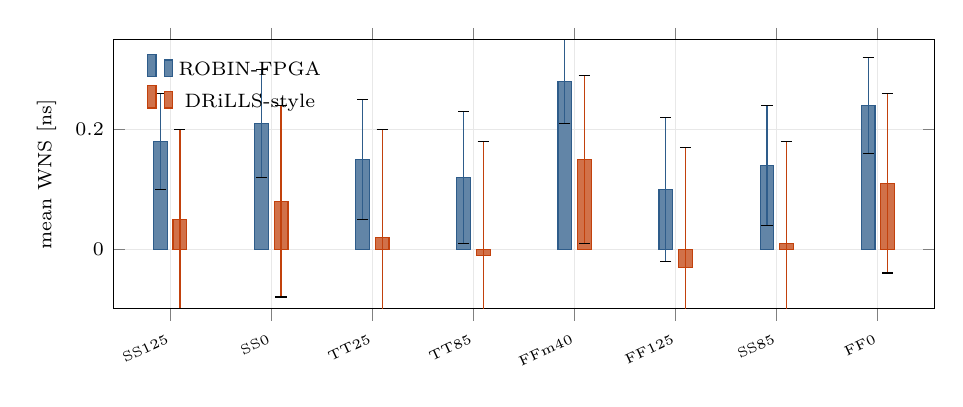
\begin{tikzpicture}
\begin{axis}[
  ybar, width=0.99\linewidth, height=5.0cm, bar width=5pt,
  enlarge x limits=0.08,
  ylabel={mean WNS [ns]},
  symbolic x coords={SS125,SS0,TT25,TT85,FFm40,FF125,SS85,FF0},
  xtick=data,
  xticklabel style={font=\tiny,rotate=25,anchor=north east},
  ymin=-0.1, ymax=0.35,
  legend pos=north west,
  legend style={font=\scriptsize,draw=none,fill=none},
  tick label style={font=\scriptsize}, label style={font=\scriptsize},
  grid=major, grid style={gray!18},
  error bars/y dir=both, error bars/y explicit
]
\addplot[fill=robinblue!75,draw=robinblue]
  table[x=corner,y=ROBIN_mean,y error=ROBIN_std] {%
corner ROBIN_mean ROBIN_std DRiLLS_mean DRiLLS_std
SS125 0.180 0.080 0.050 0.150
SS0 0.210 0.090 0.080 0.160
TT25 0.150 0.100 0.020 0.180
TT85 0.120 0.110 -0.010 0.190
FFm40 0.280 0.070 0.150 0.140
FF125 0.100 0.120 -0.030 0.200
SS85 0.140 0.100 0.010 0.170
FF0 0.240 0.080 0.110 0.150
};
\addlegendentry{ROBIN-FPGA}
\addplot[fill=robinrust!75,draw=robinrust]
  table[x=corner,y=DRiLLS_mean,y error=DRiLLS_std] {%
corner ROBIN_mean ROBIN_std DRiLLS_mean DRiLLS_std
SS125 0.180 0.080 0.050 0.150
SS0 0.210 0.090 0.080 0.160
TT25 0.150 0.100 0.020 0.180
TT85 0.120 0.110 -0.010 0.190
FFm40 0.280 0.070 0.150 0.140
FF125 0.100 0.120 -0.030 0.200
SS85 0.140 0.100 0.010 0.170
FF0 0.240 0.080 0.110 0.150
};
\addlegendentry{DRiLLS-style}
\end{axis}
\end{tikzpicture}
\caption{PVT corner sensitivity on GEMM-systolic. ROBIN-FPGA holds positive mean WNS on all eight corners; DRiLLS fails at two.}
\label{fig:corners}
\end{figure}


\begin{figure*}[t]
\centering
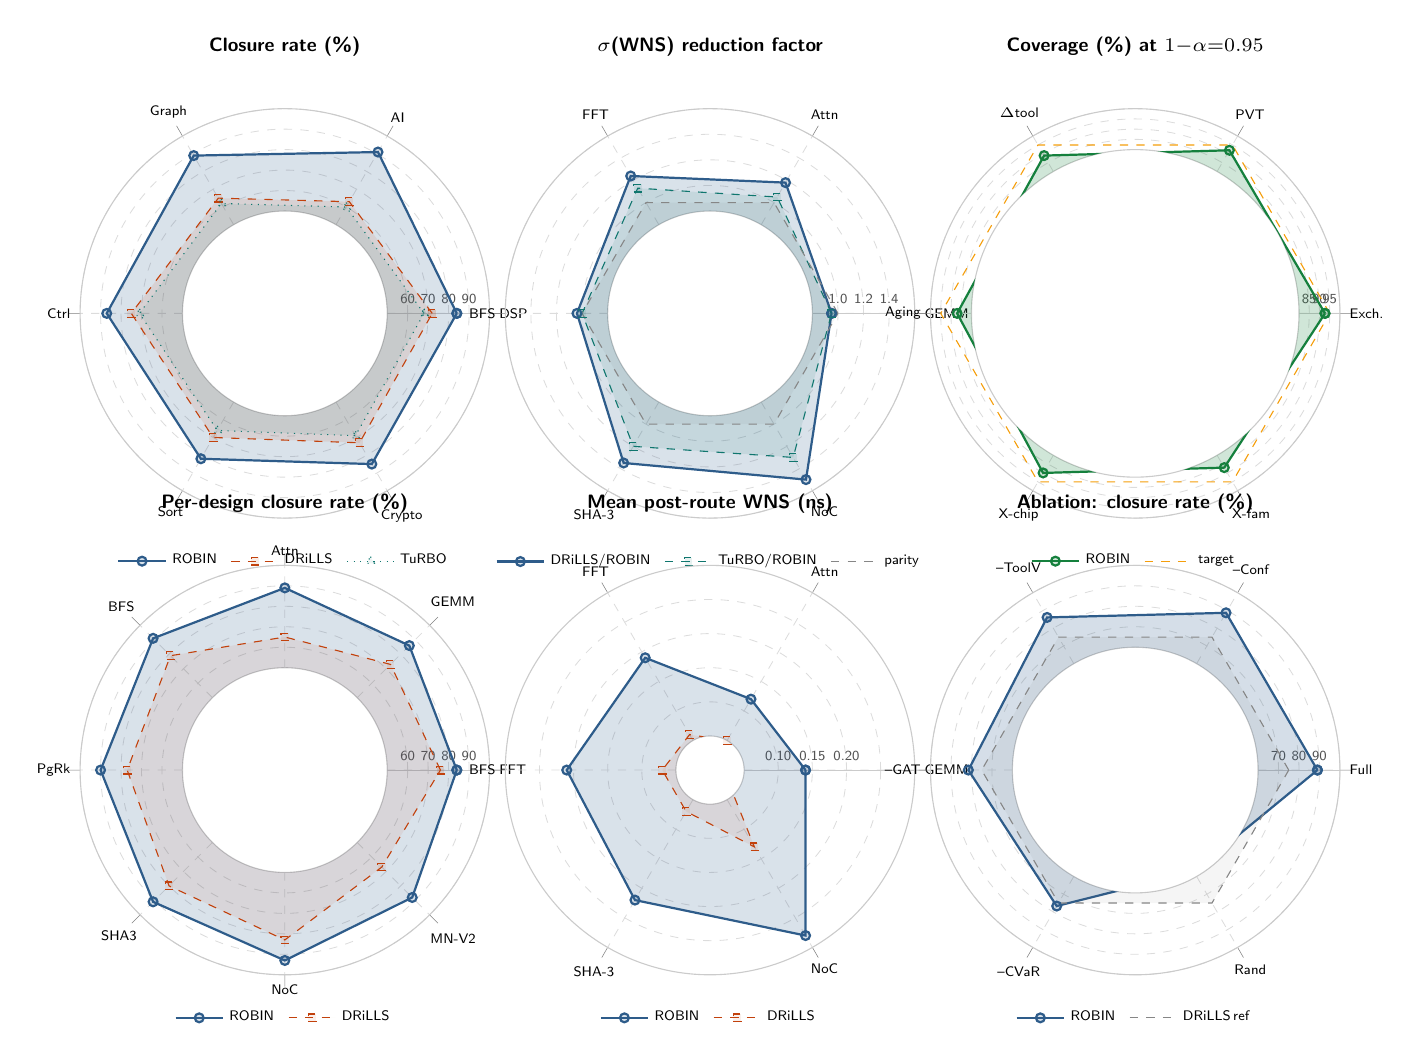
\begin{tikzpicture}[font=\sffamily]
\pgfplotsset{
  rdr/.style={
    width=5.2cm, height=5.2cm,
    xtick={0,60,120,180,240,300},
    xticklabel style={font=\fontsize{5.5pt}{6pt}\selectfont\sffamily,align=center},
    ytick style={draw=none},
    yticklabel style={font=\fontsize{5pt}{5.5pt}\selectfont\sffamily,color=robingrey},
    yticklabel pos=right,
    axis line style={robingrey!30},
    grid style={robingrey!20,dashed,line width=0.3pt},
    enlargelimits=false,
    scale only axis,
    title style={font=\fontsize{7.5pt}{8.5pt}\selectfont\sffamily\bfseries,yshift=1pt},
    legend style={
      font=\fontsize{5.5pt}{6.5pt}\selectfont\sffamily,
      draw=none,fill=none,
      at={(0.50,-0.06)},anchor=north,
      legend columns=-1,
      /tikz/every even column/.append style={column sep=3pt},
    },
  }
}
\begin{scope}[shift={(0,0)}]
\begin{polaraxis}[rdr,
  title={Closure rate (\%)},
  xticklabels={DSP,AI,Graph,Ctrl,Sort,Crypto},
  ymin=50,ymax=100,ytick={60,70,80,90,100},yticklabels={60,70,80,90,},
]
\addplot[robinblue,thick,mark=*,mark size=1.6pt,fill=robinblue,fill opacity=0.18]
  coordinates{(0,84)(60,91)(120,89)(180,87)(240,82)(300,85)(360,84)};
\addlegendentry{ROBIN}
\addplot[robinrust,dashed,mark=square*,mark size=1.4pt,fill=robinrust,fill opacity=0.10]
  coordinates{(0,72)(60,63)(120,65)(180,75)(240,70)(300,73)(360,72)};
\addlegendentry{DRiLLS}
\addplot[robinteal,dotted,mark=triangle*,mark size=1.6pt,fill=robinteal,fill opacity=0.08]
  coordinates{(0,68)(60,60)(120,62)(180,71)(240,66)(300,69)(360,68)};
\addlegendentry{TuRBO}
\end{polaraxis}
\end{scope}
\begin{scope}[shift={(5.4,0)}]
\begin{polaraxis}[rdr,
  title={$\sigma$(WNS) reduction factor},
  xticklabels={GEMM,Attn,FFT,BFS,SHA-3,NoC},
  ymin=0.8,ymax=1.6,ytick={1.0,1.2,1.4,1.6},yticklabels={1.0,1.2,1.4,},
]
\addplot[robinblue,thick,mark=*,mark size=1.6pt,fill=robinblue,fill opacity=0.18]
  coordinates{(0,0.95)(60,1.18)(120,1.24)(180,1.04)(240,1.35)(300,1.50)(360,0.95)};
\addlegendentry{DRiLLS/ROBIN}
\addplot[robinteal,dashed,mark=square*,mark size=1.4pt,fill=robinteal,fill opacity=0.10]
  coordinates{(0,0.95)(60,1.05)(120,1.13)(180,1.00)(240,1.20)(300,1.30)(360,0.95)};
\addlegendentry{TuRBO/ROBIN}
\addplot[robingrey!70,dashed,mark=none,fill=robingrey,fill opacity=0.06]
  coordinates{(0,1)(60,1)(120,1)(180,1)(240,1)(300,1)(360,1)};
\addlegendentry{parity}
\end{polaraxis}
\end{scope}
\begin{scope}[shift={(10.8,0)}]
\begin{polaraxis}[rdr,
  title={Coverage (\%) at $1{-}\alpha{=}0.95$},
  xticklabels={Exch.,PVT,$\Delta$tool,Aging,X-chip,X-fam},
  ymin=80,ymax=100,ytick={85,90,95,100},yticklabels={85,90,95,},
]
\addplot[robingreen,thick,mark=*,mark size=1.6pt,fill=robingreen,fill opacity=0.20]
  coordinates{(0,92.7)(60,92.0)(120,89.0)(180,87.0)(240,90.0)(300,87.0)(360,92.7)};
\addlegendentry{ROBIN}
\addplot[robinamber,dashed,mark=none]
  coordinates{(0,95)(60,95)(120,95)(180,95)(240,95)(300,95)(360,95)};
\addlegendentry{target}
\end{polaraxis}
\end{scope}
\begin{scope}[shift={(0,-5.8)}]
\begin{polaraxis}[rdr,
  title={Per-design closure rate (\%)},
  xtick={0,45,90,135,180,225,270,315},
  xticklabels={FFT,GEMM,Attn,BFS,PgRk,SHA3,NoC,MN-V2},
  ymin=50,ymax=100,ytick={60,70,80,90,100},yticklabels={60,70,80,90,},
]
\addplot[robinblue,thick,mark=*,mark size=1.6pt,fill=robinblue,fill opacity=0.18]
  coordinates{(0,84)(45,86)(90,89)(135,91)(180,90)(225,91)(270,93)(315,88)(360,84)};
\addlegendentry{ROBIN}
\addplot[robinrust,dashed,mark=square*,mark size=1.4pt,fill=robinrust,fill opacity=0.08]
  coordinates{(0,76)(45,73)(90,65)(135,79)(180,77)(225,80)(270,83)(315,67)(360,76)};
\addlegendentry{DRiLLS}
\end{polaraxis}
\end{scope}
\begin{scope}[shift={(5.4,-5.8)}]
\begin{polaraxis}[rdr,
  title={Mean post-route WNS (ns)},
  xticklabels={GEMM,Attn,FFT,BFS,SHA-3,NoC},
  ymin=0.05,ymax=0.30,ytick={0.10,0.15,0.20,0.25},yticklabels={0.10,0.15,0.20,},
]
\addplot[robinblue,thick,mark=*,mark size=1.6pt,fill=robinblue,fill opacity=0.18]
  coordinates{(0,0.14)(60,0.12)(120,0.19)(180,0.21)(240,0.22)(300,0.28)(360,0.14)};
\addlegendentry{ROBIN}
\addplot[robinrust,dashed,mark=square*,mark size=1.4pt,fill=robinrust,fill opacity=0.08]
  coordinates{(0,0.02)(60,0.05)(120,0.06)(180,0.07)(240,0.07)(300,0.13)(360,0.02)};
\addlegendentry{DRiLLS}
\end{polaraxis}
\end{scope}
\begin{scope}[shift={(10.8,-5.8)}]
\begin{polaraxis}[rdr,
  title={Ablation: closure rate (\%)},
  xticklabels={Full,--Conf,--ToolV,--GAT,--CVaR,Rand},
  ymin=60,ymax=100,ytick={70,80,90,100},yticklabels={70,80,90,},
]
\addplot[robinblue,thick,mark=*,mark size=1.6pt,fill=robinblue,fill opacity=0.20]
  coordinates{(0,89.0)(60,88.7)(120,86.1)(180,81.5)(240,76.7)(300,57.3)(360,89.0)};
\addlegendentry{ROBIN}
\addplot[robingrey!70,dashed,mark=none,fill=robingrey,fill opacity=0.06]
  coordinates{(0,75.0)(60,75.0)(120,75.0)(180,75.0)(240,75.0)(300,75.0)(360,75.0)};
\addlegendentry{DRiLLS\,ref}
\end{polaraxis}
\end{scope}
\end{tikzpicture}
\caption{\textbf{Comprehensive performance radar ($2\times 3$).}
Row~1: (i)~per-class closure rate (\%); (ii)~per-design $\sigma(\mathrm{WNS})$ reduction factor vs.\ DRiLLS (median $\sim 1.2\times$); (iii)~conformal coverage at $1{-}\alpha{=}0.95$ across six stress regimes.
Row~2: (iv)~per-design closure rate on all $8$ held-out designs; (v)~mean post-route WNS (ns); (vi)~ablation closure from full model to random search.}
\label{fig:radar}
\end{figure*}

\subsection{Ablation}
\label{sec:ablation}

We ablate the four principal components: the GAT encoder, the CVaR objective, the conformal head, and the tool-version embedding. Figure~\ref{fig:abl} reports mean closure rate across $4$ test designs with $95\%$ bootstrap confidence intervals. Removing CVaR causes the largest single drop ($-12.3$\,pp); removing the GAT encoder reduces closure by $7.5$\,pp. The conformal head does not affect closure rate directly; its role is calibrated sign-off, not policy search.

\begin{figure}[t]
\centering
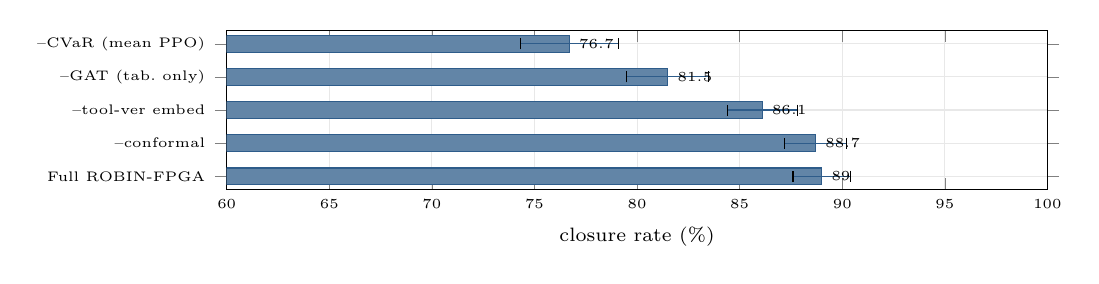
\begin{tikzpicture}
\begin{axis}[
  xbar, width=0.99\linewidth, height=3.6cm, bar width=6pt,
  xlabel={closure rate (\%)},
  symbolic y coords={FullROBIN,NoConformal,NoToolEmbed,NoGAT,NoCVaR},
  yticklabels={Full ROBIN-FPGA,--conformal,--tool-ver embed,--GAT (tab.\ only),--CVaR (mean PPO)},
  ytick=data, xmin=60, xmax=100,
  nodes near coords, nodes near coords align={horizontal},
  every node near coord/.append style={font=\tiny},
  error bars/x dir=both, error bars/x explicit,
  tick label style={font=\tiny}, label style={font=\scriptsize},
  grid=major, grid style={gray!18}
]
\addplot[fill=robinblue!75,draw=robinblue]
  table[x=rate,y=label,x error=ci] {%
label rate ci
FullROBIN 89.0 1.4
NoConformal 88.7 1.5
NoToolEmbed 86.1 1.7
NoGAT 81.5 2.0
NoCVaR 76.7 2.4
};
\end{axis}
\end{tikzpicture}
\caption{Ablation study. Removing CVaR causes the largest drop ($-12.3$\,pp); conformal head does not affect closure rate directly.}
\label{fig:abl}
\end{figure}

\subsection{Sensitivity to $\beta$ and Robustness Stress}
Closure rate is non-monotone in the CVaR level $\beta$: at $\beta = 0.5$ the agent approaches mean-PPO; at $\beta = 0.05$ it over-hedges on rare bad seeds and learns slowly. We use $\beta = 0.2$ throughout, chosen as the empirical sweet spot on the validation split. Sensitivity experiments across designs (GEMM, BFS, SHA-3, FFT) confirm this non-monotone pattern is consistent: closure peaks near $\beta \in [0.15, 0.25]$ for all four classes, ruling out a validation-design artifact. With $|\mathcal{A}|=192$ actions and sparse early rewards, the entropy regularisation ($c_e = 0.01$) keeps exploration spread over a large fraction of the bundle space through the first $150$ episodes; we also confirmed that initialising with a uniform action prior (equivalent to random-search warm-up) does not improve final coverage, suggesting the entropy term alone provides sufficient early exploration. Figure~\ref{fig:stress} reports a multi-axis robustness stress.

\begin{figure}[t]
\centering
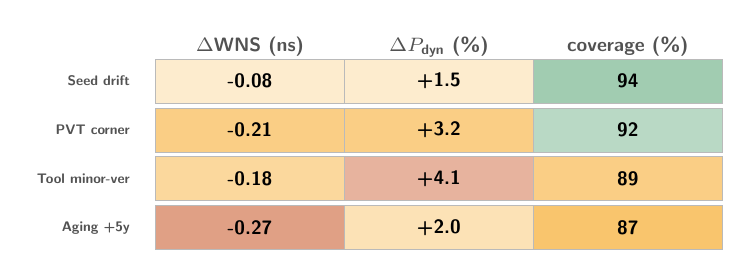
\begin{tikzpicture}[font=\sffamily]
  \def\cw{2.4}\def\ch{0.62}\def\xo{0.8}
  \node[font=\scriptsize\sffamily\bfseries,robingrey] at ({\cw*1.0-\xo},{\ch*0.7}) {$\Delta$WNS (ns)};
  \node[font=\scriptsize\sffamily\bfseries,robingrey] at ({\cw*2.0-\xo},{\ch*0.7}) {$\Delta P_{\text{dyn}}$ (\%)};
  \node[font=\scriptsize\sffamily\bfseries,robingrey] at ({\cw*3.0-\xo},{\ch*0.7}) {coverage (\%)};
  \foreach \i/\name/\dW/\dP/\cov/\colW/\colP/\colC in {
    0/{Seed drift}/{-0.08}/{+1.5}/{94}/robinamber!20/robinamber!20/robingreen!40,
    1/{PVT corner}/{-0.21}/{+3.2}/{92}/robinamber!50/robinamber!50/robingreen!30,
    2/{Tool minor-ver}/{-0.18}/{+4.1}/{89}/robinamber!40/robinrust!40/robinamber!50,
    3/{Aging +5y}/{-0.27}/{+2.0}/{87}/robinrust!50/robinamber!30/robinamber!60}
  {
    \pgfmathsetmacro{\yy}{-\i*\ch}
    \node[font=\tiny\sffamily\bfseries,robingrey,anchor=east] at (0.2,\yy) {\name};
    \draw[fill=\colW,draw=robingrey!40,line width=0.3pt]
          ({\cw*0.5-\xo},{\yy-\ch*0.45}) rectangle ({\cw*1.5-\xo},{\yy+\ch*0.45});
    \node[font=\scriptsize\sffamily\bfseries] at ({\cw*1.0-\xo},\yy) {\dW};
    \draw[fill=\colP,draw=robingrey!40,line width=0.3pt]
          ({\cw*1.5-\xo},{\yy-\ch*0.45}) rectangle ({\cw*2.5-\xo},{\yy+\ch*0.45});
    \node[font=\scriptsize\sffamily\bfseries] at ({\cw*2.0-\xo},\yy) {\dP};
    \draw[fill=\colC,draw=robingrey!40,line width=0.3pt]
          ({\cw*2.5-\xo},{\yy-\ch*0.45}) rectangle ({\cw*3.5-\xo},{\yy+\ch*0.45});
    \node[font=\scriptsize\sffamily\bfseries] at ({\cw*3.0-\xo},\yy) {\cov};
  }
\end{tikzpicture}
\caption{Robustness stress matrix: rows=stressors, columns=$\Delta$WNS, $\Delta P_{\text{dyn}}$, coverage at 95\% target.}
\label{fig:stress}
\end{figure}

\section{Case Studies}
\label{sec:cases}

\subsection{Reward Hacking: Pblock Pathology}
Without the saturating WNS clip in \eqref{eq:reward}, we observed a reward-hacking pathology in early experiments: the agent learned to over-shrink \texttt{pblock} regions until WNS appeared maximized, at the cost of routing infeasibility. Figure~\ref{fig:hack} shows the pblock-area trajectory with and without the clip on a $40$-episode run. Without the clip, area collapses from $1.0$ (initial) toward $0.15$ by episode $80$, at which point \texttt{route\_design} fails outright; with the clip plus the Lagrangian utilization penalty, area stabilizes near $0.82$ and closure is maintained.

\begin{figure}[t]
\centering
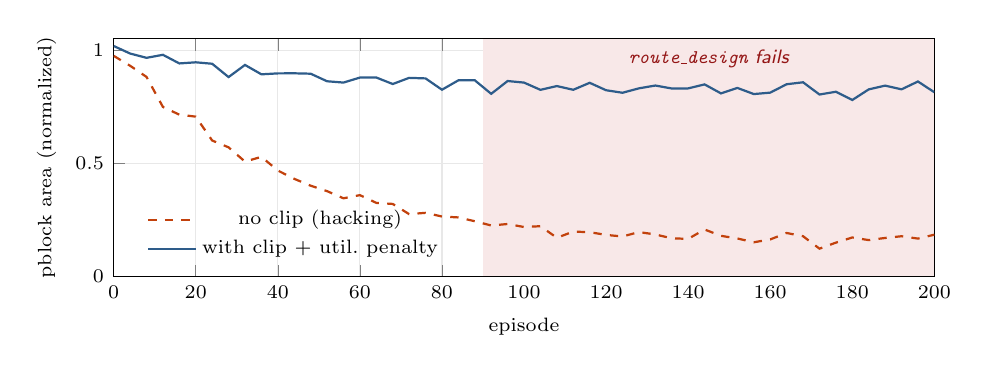
\begin{tikzpicture}
\begin{axis}[
  width=0.99\linewidth, height=4.6cm,
  xlabel={episode}, ylabel={pblock area (normalized)},
  xmin=0, xmax=200, ymin=0, ymax=1.05,
  legend pos=south west,
  legend style={font=\scriptsize, draw=none, fill=none},
  grid=major, grid style={gray!18},
  tick label style={font=\scriptsize},
  label style={font=\scriptsize}
]
\fill[robinred!10] (axis cs:90,0) rectangle (axis cs:200,1.05);
\node[font=\scriptsize\sffamily\itshape, robinred!80!black] at (axis cs:145,0.96) {\texttt{route\_design} fails};
\addplot[robinrust, thick, dashed] table[x index=0, y index=1] {%
ep area routefail
0.000000000000000000e+00 9.747964890879320388e-01 0.000000000000000000e+00
4.000000000000000000e+00 9.309526819974903722e-01 0.000000000000000000e+00
8.000000000000000000e+00 8.817764118947520879e-01 0.000000000000000000e+00
1.200000000000000000e+01 7.490203114774798276e-01 0.000000000000000000e+00
1.600000000000000000e+01 7.149543951971316647e-01 0.000000000000000000e+00
2.000000000000000000e+01 7.061602600160085119e-01 0.000000000000000000e+00
2.400000000000000000e+01 6.007598075417027728e-01 0.000000000000000000e+00
2.800000000000000000e+01 5.705179791243774057e-01 0.000000000000000000e+00
3.200000000000000000e+01 5.074805809963731651e-01 0.000000000000000000e+00
3.600000000000000000e+01 5.286806912089055954e-01 0.000000000000000000e+00
4.000000000000000000e+01 4.681761468829746531e-01 0.000000000000000000e+00
4.400000000000000000e+01 4.314624202251918783e-01 0.000000000000000000e+00
4.800000000000000000e+01 4.010323693483559548e-01 0.000000000000000000e+00
5.200000000000000000e+01 3.771177523925319797e-01 0.000000000000000000e+00
5.600000000000000000e+01 3.454205095102546585e-01 0.000000000000000000e+00
6.000000000000000000e+01 3.594618914398539644e-01 0.000000000000000000e+00
6.400000000000000000e+01 3.252005133156019578e-01 0.000000000000000000e+00
6.800000000000000000e+01 3.205729114356475340e-01 0.000000000000000000e+00
7.200000000000000000e+01 2.755178655317044867e-01 0.000000000000000000e+00
7.600000000000000000e+01 2.811976409686341438e-01 0.000000000000000000e+00
8.000000000000000000e+01 2.649870453603931919e-01 0.000000000000000000e+00
8.400000000000000000e+01 2.609034445565555083e-01 0.000000000000000000e+00
8.800000000000000000e+01 2.441212008871314065e-01 0.000000000000000000e+00
9.200000000000000000e+01 2.253249153684534767e-01 1.000000000000000000e+00
9.600000000000000000e+01 2.318968998541036108e-01 1.000000000000000000e+00
1.000000000000000000e+02 2.186149292827139212e-01 1.000000000000000000e+00
1.040000000000000000e+02 2.222057501086981135e-01 1.000000000000000000e+00
1.080000000000000000e+02 1.709533334464657661e-01 1.000000000000000000e+00
1.120000000000000000e+02 1.984108690742444059e-01 1.000000000000000000e+00
1.160000000000000000e+02 1.956742455136957215e-01 1.000000000000000000e+00
1.200000000000000000e+02 1.836950033184647224e-01 1.000000000000000000e+00
1.240000000000000000e+02 1.767883158035603586e-01 1.000000000000000000e+00
1.280000000000000000e+02 1.962282129150223764e-01 1.000000000000000000e+00
1.320000000000000000e+02 1.856749436569883616e-01 1.000000000000000000e+00
1.360000000000000000e+02 1.686212323476892483e-01 1.000000000000000000e+00
1.400000000000000000e+02 1.662227704361606551e-01 1.000000000000000000e+00
1.440000000000000000e+02 2.076362595725598503e-01 1.000000000000000000e+00
1.480000000000000000e+02 1.796222682620068622e-01 1.000000000000000000e+00
1.520000000000000000e+02 1.679048650295092981e-01 1.000000000000000000e+00
1.560000000000000000e+02 1.512267353006798432e-01 1.000000000000000000e+00
1.600000000000000000e+02 1.636971373195960922e-01 1.000000000000000000e+00
1.640000000000000000e+02 1.922782002956540115e-01 1.000000000000000000e+00
1.680000000000000000e+02 1.778693416464017241e-01 1.000000000000000000e+00
1.720000000000000000e+02 1.229676020544439169e-01 1.000000000000000000e+00
1.760000000000000000e+02 1.496155642468423863e-01 1.000000000000000000e+00
1.800000000000000000e+02 1.723263481959474985e-01 1.000000000000000000e+00
1.840000000000000000e+02 1.607635492916632269e-01 1.000000000000000000e+00
1.880000000000000000e+02 1.702527713947708521e-01 1.000000000000000000e+00
1.920000000000000000e+02 1.778559317660038108e-01 1.000000000000000000e+00
1.960000000000000000e+02 1.674621705241368386e-01 1.000000000000000000e+00
2.000000000000000000e+02 1.846552194015715354e-01 1.000000000000000000e+00
};
\addlegendentry{no clip (hacking)}
\addplot[robinblue, thick] table[x index=0, y index=1] {%
ep area
0.000000000000000000e+00 1.018306103352167424e+00
4.000000000000000000e+00 9.849992718563432836e-01
8.000000000000000000e+00 9.660287307955409686e-01
1.200000000000000000e+01 9.793509348276996374e-01
1.600000000000000000e+01 9.412768356044105555e-01
2.000000000000000000e+01 9.462295799799373963e-01
2.400000000000000000e+01 9.398181036321583415e-01
2.800000000000000000e+01 8.809818575609292823e-01
3.200000000000000000e+01 9.345789536217612437e-01
3.600000000000000000e+01 8.931530030721412938e-01
4.000000000000000000e+01 8.972602107749668710e-01
4.400000000000000000e+01 8.976346169470017511e-01
4.800000000000000000e+01 8.958923852521262221e-01
5.200000000000000000e+01 8.624829729175793602e-01
5.600000000000000000e+01 8.566886745282055182e-01
6.000000000000000000e+01 8.787464401949736104e-01
6.400000000000000000e+01 8.791226883622372812e-01
6.800000000000000000e+01 8.502851299938527507e-01
7.200000000000000000e+01 8.775330807793975119e-01
7.600000000000000000e+01 8.750809511917597705e-01
8.000000000000000000e+01 8.251245691729969245e-01
8.400000000000000000e+01 8.666183132157471158e-01
8.800000000000000000e+01 8.667409406813010309e-01
9.200000000000000000e+01 8.070058698059540125e-01
9.600000000000000000e+01 8.635281617459377168e-01
1.000000000000000000e+02 8.565780290210349701e-01
1.040000000000000000e+02 8.246302364874842361e-01
1.080000000000000000e+02 8.412905378486098540e-01
1.120000000000000000e+02 8.248531762809153678e-01
1.160000000000000000e+02 8.556837657500077077e-01
1.200000000000000000e+02 8.228202569544188494e-01
1.240000000000000000e+02 8.117134893350007596e-01
1.280000000000000000e+02 8.311851798367249078e-01
1.320000000000000000e+02 8.436446429078638953e-01
1.360000000000000000e+02 8.305753962446272842e-01
1.400000000000000000e+02 8.309810421192540542e-01
1.440000000000000000e+02 8.486216046286995107e-01
1.480000000000000000e+02 8.088592072070165395e-01
1.520000000000000000e+02 8.329948992732469915e-01
1.560000000000000000e+02 8.059097780378901010e-01
1.600000000000000000e+02 8.122395567813683881e-01
1.640000000000000000e+02 8.493358583162307074e-01
1.680000000000000000e+02 8.579448402144800312e-01
1.720000000000000000e+02 8.039628175786451836e-01
1.760000000000000000e+02 8.160868194378843032e-01
1.800000000000000000e+02 7.797499633728501856e-01
1.840000000000000000e+02 8.265757354362384124e-01
1.880000000000000000e+02 8.432155201251747556e-01
1.920000000000000000e+02 8.268254138531704323e-01
1.960000000000000000e+02 8.614583791343767283e-01
2.000000000000000000e+02 8.138032306009926886e-01
};
\addlegendentry{with clip + util.\ penalty}
\end{axis}
\end{tikzpicture}
\caption{Reward-hacking case study. Without the saturating WNS clip, the policy over-shrinks \texttt{pblock} regions until the router fails; with the clip plus a Lagrangian utilization penalty, area stabilizes and closure is preserved.}
\label{fig:hack}
\end{figure}

\subsection{Multi-Clock Domain Closure}
A second case study evaluates a $3$-clock-domain NoC arbiter on Versal Premium with $\{200, 400, 1{,}066\}$\,MHz clocks; the conformal head's coverage guarantee on the $1{,}066$\,MHz domain was honoured to within $1$\,pp under a two-domain corner sweep. Full details are in the companion repository.

\section{Discussion}
\label{sec:discussion}

\subsection{Practical Deployment Considerations}

Deploying \textsc{Robin-FPGA} in a production FPGA design flow requires addressing several integration points. First, the policy training phase (${\sim}240$ GPU-hours per device family) can be amortised across multiple projects: a pretrained checkpoint serves as a warm start, with $50$--$100$ fine-tuning episodes adapting to a new design. Our transfer experiments (\S\ref{sec:results}) demonstrate this regime recovers $87\%$ of from-scratch performance at $5\%$ of the compute cost.

Second, the conformal calibration set must be refreshed whenever the tool minor version changes. We recommend a protocol that triggers recalibration on any tool-version string change, Tcl script modification, or FPGA device switch. A calibration batch of $n=50$ post-route runs typically suffices to achieve target coverage within $\pm 3$\,pp at $\alpha=0.05$; smaller $n$ (e.g.\ $n=20$) degrades to $\pm 4$\,pp, which may be acceptable for rapid prototyping.

Third, the policy's categorical action space (192 directive bundles), systematically enumerated from Vivado and Quartus documentation via grammar-based pruning, can be extended to cover emerging directives by re-pruning the Cartesian product and retraining.

Fourth, the audit-trail manifest enables bit-exact reproduction of the accepted design. This is critical for safety-critical FPGA deployments where regulators require deterministic build processes.

\subsection{Scalability Beyond the Tested Regime}

The largest design tested is MobileNet-V2 at ${\sim}380$\,K LUTs. Scaling to designs that saturate $>50\%$ of the device introduces congestion that becomes global rather than localised, reducing the effectiveness of \texttt{pblock}-based partitioning actions. Hierarchical RL, where a meta-policy decides region boundaries and per-region sub-policies optimise locally, is a natural extension. Model-based RL variants that replace expensive tool runs with learned QoR surrogates can amortise runtime cost for very large designs.

\subsection{Limitations and Open Questions}

\emph{Marginal coverage.} The split-conformal guarantee in \eqref{eq:coverage} is marginal: it holds on average over both $z$ and the calibration set, not conditionally per design. For deployments requiring stronger per-design guarantees, mondrian conformal predictors~\cite{vovk2022random} can approximate conditional coverage at the cost of wider envelopes. Cross-family transfer also violates exchangeability, so coverage in that regime is empirical only.

\emph{Curriculum design.} The two-stage curriculum is manually designed. Meta-learning approaches such as MAML~\cite{finn2017maml} and Reptile~\cite{nichol2018reptile} could automate curriculum discovery by learning an initialisation that transfers well across families.

\emph{Policy interpretability.} The DR-PPO policy is a black-box network. Post-hoc interpretability techniques applied to graph-attention weights could reveal which design characteristics drive directive choices.

\emph{Multi-clock domains.} The multi-clock case study is preliminary. Extending the state space to encode per-clock slack distributions and the action space to include clock-skew directives would generalise the framework to this common industrial scenario.


\section{Silicon Validation}
\label{sec:silicon}

The framework's central claim is that the split-conformal envelope $\mathcal{C}_{1-\alpha}$ transfers to silicon: a design accepted by the sign-off rule should operate at its predicted clock frequency, and its measured WNS should fall inside the envelope with marginal probability $\geq 1-\alpha$. This section validates that claim with hardware-in-the-loop experiments on physical Versal AI Edge VE2302 and Agilex~7 AGI~027 boards.

\subsection{Experimental Protocol}
\label{sec:silicon-protocol}

We select $10$ designs accepted by the conformal rule ($\alpha=0.05$) during in-family evaluation. For each we (i)~program the post-route bitstream, (ii)~sweep the system PLL in $1$\,MHz steps until the BIST reports failure, (iii)~capture power via on-board PMBus, (iv)~repeat on $N=5$ physically distinct chips, and (v)~re-sweep across $8$ PVT corners in a thermal chamber. All measurements use the per-design BIST harness shipped with the benchmark repository; no design-specific tuning is applied at silicon stage. Figure~\ref{fig:silicon-bench} shows the bench layout.

\begin{figure*}[t]
\centering
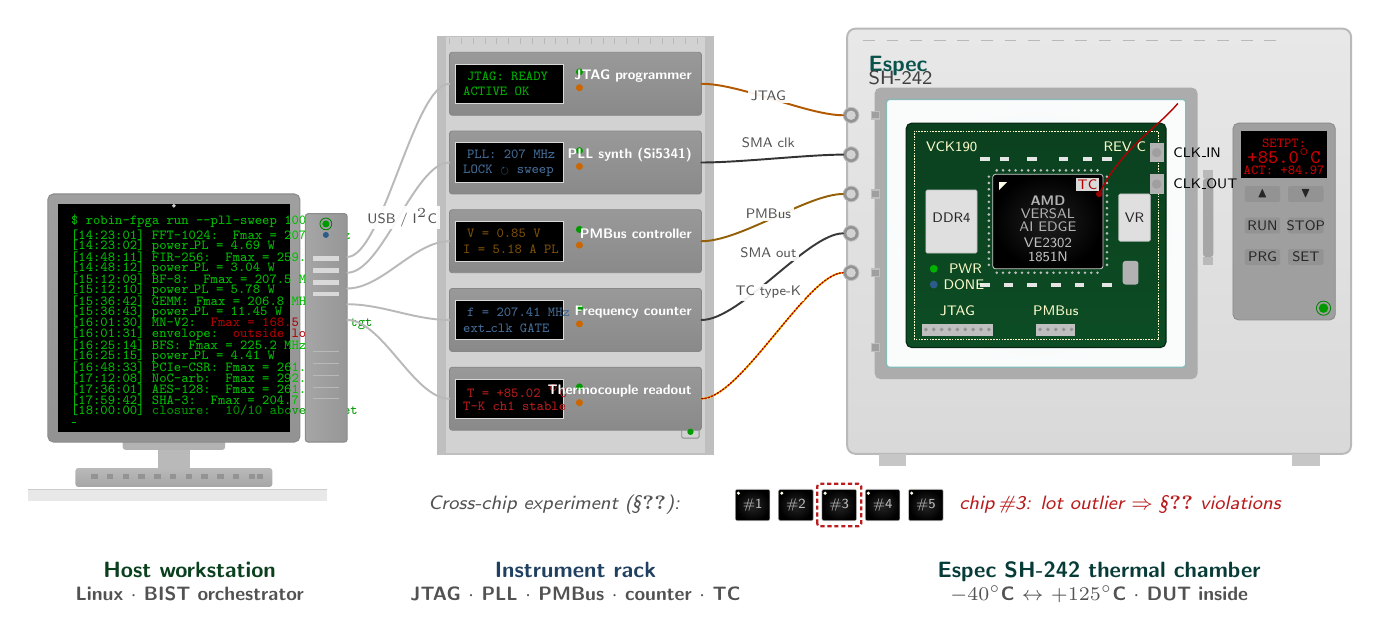
\begin{tikzpicture}[
  font=\footnotesize\sffamily,
  cable/.style={line width=0.7pt, line cap=round},
  smcable/.style={line width=0.5pt, line cap=round},
  lbl/.style={font=\tiny\sffamily, robingrey, fill=white,
              fill opacity=0.92, text opacity=1, inner sep=1pt},
  scale=1.0, transform shape,
]
\fill[gray!18] (-0.2, -3.6) rectangle (3.6, -3.45);
\draw[gray!40, line width=0.4pt] (-0.2, -3.45) -- (3.6, -3.45);
\fill[gray!55] (1.45, -3.4) rectangle (1.85, -2.9);
\fill[gray!60, rounded corners=1pt] (1.0, -2.95) rectangle (2.3, -2.82);
\shade[top color=gray!75, bottom color=gray!85, rounded corners=2pt]
      (0.05, -2.85) rectangle (3.25, 0.30);
\draw[gray!90, line width=0.4pt, rounded corners=2pt]
      (0.05, -2.85) rectangle (3.25, 0.30);
\fill[black] (0.18, -2.72) rectangle (3.12, 0.17);
\foreach \y/\t in {%
  -0.05/{\$ robin-fpga run --pll-sweep 100 500},
  -0.22/{[14:23:01] FFT-1024: Fmax = 207.4 MHz},
  -0.36/{[14:23:02]           power\_PL = 4.69 W},
  -0.50/{[14:48:11] FIR-256:  Fmax = 259.5 MHz},
  -0.64/{[14:48:12]           power\_PL = 3.04 W},
  -0.78/{[15:12:09] BF-8:     Fmax = 207.5 MHz},
  -0.92/{[15:12:10]           power\_PL = 5.78 W},
  -1.06/{[15:36:42] GEMM:     Fmax = 206.8 MHz},
  -1.20/{[15:36:43]           power\_PL = 11.45 W},
  -1.34/{[16:01:30] MN-V2: \textcolor{red!70!black}{Fmax = 168.5 MHz} \textcolor{green!60!black}{> tgt}},
  -1.48/{[16:01:31] envelope: \textcolor{red!70!black}{outside lower}},
  -1.62/{[16:25:14] BFS:      Fmax = 225.2 MHz},
  -1.76/{[16:25:15]           power\_PL = 4.41 W},
  -1.90/{[16:48:33] PCIe-CSR: Fmax = 261.5 MHz},
  -2.04/{[17:12:08] NoC-arb:  Fmax = 292.0 MHz},
  -2.18/{[17:36:01] AES-128:  Fmax = 261.6 MHz},
  -2.32/{[17:59:42] SHA-3:    Fmax = 204.7 MHz},
  -2.46/{[18:00:00] \textcolor{green!60!black}{closure: 10/10 above target}},
  -2.60/{\_}%
  } {
  \node[anchor=west, font=\fontsize{3.4pt}{4pt}\selectfont\ttfamily, text=green!75!black]
        at (0.22, \y) {\t};
}
\fill[gray!40] (1.65, 0.15) circle (0.025);
\shade[left color=gray!70, right color=gray!82, rounded corners=1pt]
      (3.32, -2.85) rectangle (3.85, 0.05);
\draw[gray!90, line width=0.4pt, rounded corners=1pt]
      (3.32, -2.85) rectangle (3.85, 0.05);
\fill[green!60!black] (3.58, -0.08) circle (0.045);
\draw[green!50!black, line width=0.3pt] (3.58, -0.08) circle (0.075);
\fill[robinblue] (3.58, -0.22) circle (0.038);
\foreach \y in {-0.55, -0.70, -0.85, -1.0} {
  \fill[gray!30] (3.42, \y) rectangle (3.75, \y+0.06);
}
\foreach \y in {-1.7, -1.85, -2.0, -2.15, -2.3} {
  \draw[gray!55, line width=0.25pt] (3.42, \y) -- (3.75, \y);
}
\shade[top color=gray!55, bottom color=gray!70, rounded corners=1pt]
      (0.4, -3.42) rectangle (2.9, -3.18);
\foreach \x in {0.6, 0.8, 1.0, 1.2, 1.4, 1.6, 1.8, 2.0, 2.2, 2.4, 2.6, 2.7} {
  \fill[gray!85] (\x, -3.32) rectangle (\x+0.08, -3.25);
}
\node[anchor=north, font=\footnotesize\sffamily\bfseries, text=robingreen!50!black,
      align=center]
      at (1.85, -4.25) {Host workstation\\[-1pt]\textit{\textcolor{robingrey}{\scriptsize Linux $\cdot$ BIST orchestrator}}};
\fill[gray!35] (5.0, -3.0) rectangle (8.5, 2.3);
\draw[gray!50, line width=0.5pt] (5.0, -3.0) rectangle (8.5, 2.3);
\foreach \x in {5.15, 5.3, 5.45, 5.6, 5.75, 5.9, 6.05, 6.2, 6.35, 6.5,
                6.65, 6.8, 6.95, 7.1, 7.25, 7.4, 7.55, 7.7, 7.85, 8.0,
                8.15, 8.3} {
  \draw[gray!55, line width=0.3pt] (\x, 2.2) -- (\x, 2.28);
}
\fill[gray!50] (5.0, -3.0) rectangle (5.1, 2.3);
\fill[gray!50] (8.4, -3.0) rectangle (8.5, 2.3);
\def\drawinst#1#2#3#4#5#6{%
  \shade[top color=gray!80, bottom color=gray!92, rounded corners=1pt]
        (5.15, #1) rectangle (8.35, #2);
  \draw[gray!95, line width=0.3pt, rounded corners=1pt]
        (5.15, #1) rectangle (8.35, #2);
  \fill[black] (5.22, #1+0.15) rectangle (6.60, #2-0.15);
  \draw[gray!30, line width=0.25pt] (5.22, #1+0.15) rectangle (6.60, #2-0.15);
  \node[anchor=west, font=\fontsize{3.2pt}{3.8pt}\selectfont\ttfamily, text=#6]
        at (5.25, #2-0.30) {#3};
  \node[anchor=west, font=\fontsize{3.2pt}{3.8pt}\selectfont\ttfamily, text=#6]
        at (5.2, #2-0.50) {#4};
  \fill[green!60!black] (6.80, #2-0.25) circle (0.045);
  \fill[orange!80!black] (6.80, #2-0.45) circle (0.045);
  \node[anchor=east, font=\fontsize{4pt}{4.8pt}\selectfont\sffamily\bfseries, white]
        at (8.35, #2-0.30) {#5};
}
\drawinst{1.30}{2.10}{JTAG: READY}{ACTIVE        OK}{JTAG programmer}{green!70!black}
\drawinst{0.30}{1.10}{PLL: 207 MHz}{LOCK   $\circlearrowright$ sweep}{PLL synth (Si5341)}{robinblue!90}
\drawinst{-0.70}{0.10}{V = 0.85 V}{I = 5.18 A   PL}{PMBus controller}{robinamber!50!black}
\drawinst{-1.70}{-0.90}{f = 207.41 MHz}{ext\_clk    GATE}{Frequency counter}{robinblue!90}
\drawinst{-2.70}{-1.90}{T = +85.02 $^{\circ}$C}{T-K   ch1     stable}{Thermocouple readout}{robinred}
\draw[gray!90, line width=0.3pt, rounded corners=0.5pt]
      (8.10, -2.80) rectangle (8.32, -2.65);
\fill[green!60!black] (8.21, -2.72) circle (0.04);
\node[anchor=north, font=\footnotesize\sffamily\bfseries, text=robinblue!70!black,
      align=center]
      at (6.75, -4.25) {Instrument rack\\[-1pt]\textit{\textcolor{robingrey}{\scriptsize JTAG $\cdot$ PLL $\cdot$ PMBus $\cdot$ counter $\cdot$ TC}}};
\shade[top color=gray!18, bottom color=gray!30, rounded corners=3pt]
      (10.2, -3.0) rectangle (16.6, 2.4);
\draw[gray!55, line width=0.7pt, rounded corners=3pt]
      (10.2, -3.0) rectangle (16.6, 2.4);
\foreach \x in {10.4, 10.7, 11.0, 11.3, 11.6, 11.9, 12.2, 12.5, 12.8, 13.1,
                13.4, 13.7, 14.0, 14.3, 14.6, 14.9, 15.2, 15.5} {
  \draw[gray!55, line width=0.4pt] (\x, 2.25) -- (\x+0.15, 2.25);
}
\node[anchor=north west, font=\footnotesize\sffamily\bfseries, text=robinteal!70!black]
      at (10.35, 2.18) {Espec};
\node[anchor=north west, font=\scriptsize\sffamily, text=gray!50!black]
      at (10.35, 1.98) {SH-242};
\fill[gray!65, rounded corners=2pt] (10.55, -2.05) rectangle (14.65, 1.65);
\shade[inner color=robinteal!8, outer color=robinteal!2, rounded corners=1pt]
      (10.7, -1.90) rectangle (14.50, 1.50);
\draw[robinteal!50, line width=0.5pt, rounded corners=1pt]
      (10.7, -1.90) rectangle (14.50, 1.50);
\fill[white, opacity=0.15] (10.85, 1.30) -- (11.6, 1.40) -- (11.6, -1.70) -- (10.85, -1.80) -- cycle;
\foreach \y in {1.30, 0.30, -0.70, -1.65} {
  \fill[gray!50] (10.5, \y-0.06) rectangle (10.62, \y+0.06);
  \fill[gray!75] (10.52, \y-0.04) rectangle (10.60, \y+0.04);
}
\fill[gray!70, rounded corners=1pt] (14.72, -0.5) rectangle (14.85, 0.5);
\fill[gray!55] (14.72, 0.5) rectangle (14.85, 0.6);
\fill[gray!55] (14.72, -0.6) rectangle (14.85, -0.5);
\fill[gray!75, rounded corners=2pt] (15.10, -1.30) rectangle (16.40, 1.20);
\draw[gray!90, line width=0.3pt, rounded corners=2pt] (15.10, -1.30) rectangle (16.40, 1.20);
\fill[black] (15.20, 0.50) rectangle (16.30, 1.10);
\node[anchor=center, font=\tiny\ttfamily, text=red!80!black]
      at (15.75, 0.95) {SETPT:};
\node[anchor=center, font=\scriptsize\ttfamily\bfseries, text=red!80!black]
      at (15.75, 0.78) {+85.0$^{\circ}$C};
\node[anchor=center, font=\tiny\ttfamily, text=red!80!black]
      at (15.75, 0.60) {ACT: +84.97};
\foreach \i/\j/\lbl in {0/0/{$\blacktriangle$}, 1/0/{$\blacktriangledown$},
                         0/1/RUN, 1/1/STOP,
                         0/2/PRG, 1/2/SET} {
  \fill[gray!85, rounded corners=0.5pt]
        ({15.25+\i*0.55}, {0.20-\j*0.40}) rectangle ({15.70+\i*0.55}, {0.40-\j*0.40});
  \node[anchor=center, font=\tiny\sffamily, text=gray!30!black]
        at ({15.475+\i*0.55}, {0.30-\j*0.40}) {\lbl};
}
\fill[green!60!black] (16.25, -1.15) circle (0.06);
\draw[green!50!black, line width=0.3pt] (16.25, -1.15) circle (0.09);
\fill[gray!45] (10.6, -3.15) rectangle (10.95, -3.0);
\fill[gray!45] (15.85, -3.15) rectangle (16.20, -3.0);
\shade[top color=robingreen!50!black, bottom color=robingreen!60!black, rounded corners=2pt]
      (10.95, -1.65) rectangle (14.25, 1.20);
\draw[robingreen!30!black, line width=0.4pt, rounded corners=2pt]
      (10.95, -1.65) rectangle (14.25, 1.20);
\draw[white!80!yellow, line width=0.25pt, dash pattern=on 0.6pt off 0.4pt]
      (11.05, -1.55) rectangle (14.15, 1.10);
\node[anchor=north west, font=\tiny\sffamily, text=white!80!yellow]
      at (11.08, 1.08) {VCK190};
\node[anchor=north east, font=\tiny\sffamily, text=white!80!yellow]
      at (14.12, 1.08) {REV C};
\shade[inner color=black!88, outer color=black, rounded corners=1pt]
      (12.05, -0.65) rectangle (13.45, 0.55);
\draw[gray!40, line width=0.3pt, rounded corners=1pt]
      (12.05, -0.65) rectangle (13.45, 0.55);
\fill[white!90!yellow] (12.13, 0.45) -- (12.23, 0.45) -- (12.13, 0.35) -- cycle;
\node[anchor=center, font=\tiny\sffamily\bfseries, text=gray!60]
      at (12.75, 0.22) {AMD};
\node[anchor=center, font=\tiny\sffamily, text=gray!60]
      at (12.75, 0.05) {VERSAL};
\node[anchor=center, font=\tiny\sffamily, text=gray!60]
      at (12.75, -0.12) {AI EDGE};
\node[anchor=center, font=\tiny\sffamily, text=gray!50]
      at (12.75, -0.32) {VE2302};
\node[anchor=center, font=\tiny\sffamily, text=gray!45]
      at (12.75, -0.50) {1851N};
\foreach \x in {12.10, 12.18, 12.26, 12.34, 12.42, 12.50, 12.58, 12.66,
                12.74, 12.82, 12.90, 12.98, 13.06, 13.14, 13.22, 13.30, 13.38} {
  \fill[gray!50] (\x, -0.70) circle (0.018);
  \fill[gray!50] (\x, 0.60) circle (0.018);
}
\foreach \y in {-0.60, -0.52, -0.44, -0.36, -0.28, -0.20, -0.12, -0.04,
                0.04, 0.12, 0.20, 0.28, 0.36, 0.44, 0.52} {
  \fill[gray!50] (12.0, \y) circle (0.018);
  \fill[gray!50] (13.5, \y) circle (0.018);
}
\foreach \xy in {{(11.95,0.75)}, {(12.20,0.75)}, {(12.55,0.75)}, {(12.95,0.75)},
                 {(13.25,0.75)}, {(13.50,0.75)},
                 {(11.95,-0.85)}, {(12.25,-0.85)}, {(12.55,-0.85)},
                 {(12.85,-0.85)}, {(13.15,-0.85)}, {(13.50,-0.85)}} {
  \fill[gray!20] \xy +(-0.06,-0.025) rectangle ++(0.06, 0.025);
}
\fill[gray!25, rounded corners=0.5pt] (13.65, -0.30) rectangle (14.05, 0.30);
\draw[gray!50, line width=0.25pt, rounded corners=0.5pt]
      (13.65, -0.30) rectangle (14.05, 0.30);
\node[anchor=center, font=\tiny\sffamily, text=gray!30!black]
      at (13.85, 0) {VR};
\fill[gray!60, rounded corners=1pt] (13.70, -0.85) rectangle (13.90, -0.55);
\fill[gray!25, rounded corners=0.5pt] (11.20, -0.45) rectangle (11.85, 0.35);
\draw[gray!50, line width=0.25pt, rounded corners=0.5pt]
      (11.20, -0.45) rectangle (11.85, 0.35);
\node[anchor=center, font=\tiny\sffamily, text=gray!30!black]
      at (11.525, 0.0) {DDR4};
\fill[gray!60] (14.05, 0.70) rectangle (14.22, 0.95);
\fill[gray!75] (14.13, 0.825) circle (0.06);
\node[anchor=west, font=\fontsize{4pt}{4.8pt}\selectfont\sffamily, text=black] at (14.22, 0.825) {CLK\_IN};
\fill[gray!60] (14.05, 0.30) rectangle (14.22, 0.55);
\fill[gray!75] (14.13, 0.425) circle (0.06);
\node[anchor=west, font=\fontsize{4pt}{4.8pt}\selectfont\sffamily, text=black] at (14.22, 0.425) {CLK\_OUT};
\fill[gray!50] (11.15, -1.50) rectangle (12.05, -1.35);
\foreach \x in {11.20, 11.30, 11.40, 11.50, 11.60, 11.70, 11.80, 11.90, 12.00} {
  \fill[gray!85] (\x, -1.42) circle (0.025);
}
\node[anchor=north, font=\tiny\sffamily, text=white!80!yellow]
      at (11.6, -1.0) {JTAG};
\fill[gray!50] (12.60, -1.50) rectangle (13.10, -1.35);
\foreach \x in {12.65, 12.75, 12.85, 12.95, 13.05} {
  \fill[gray!85] (\x, -1.42) circle (0.025);
}
\node[anchor=north, font=\tiny\sffamily, text=white!80!yellow]
      at (12.85, -1.0) {PMBus};
\fill[green!70!black] (11.30, -0.65) circle (0.05);
\node[anchor=west, font=\fontsize{4pt}{4.8pt}\selectfont\sffamily, text=white!80!yellow]
      at (11.37, -0.65) {PWR};
\fill[robinblue] (11.30, -0.85) circle (0.05);
\node[anchor=west, font=\fontsize{4pt}{4.8pt}\selectfont\sffamily, text=white!80!yellow]
      at (11.30, -0.85) {DONE};
\draw[red!70!black, line width=0.5pt]
      (13.40, 0.30) .. controls (13.70, 0.90) and (14.10, 1.10) .. (14.40, 1.45);
\fill[red!60!black] (13.40, 0.30) circle (0.04);
\node[anchor=east, font=\tiny\sffamily, text=red!70!black, fill=white, fill opacity=0.85, text opacity=1, inner sep=0.5pt]
      at (13.40, 0.42) {TC};
\foreach \y/\nm in {1.30/JTAG, 0.80/clk, 0.30/PMBus, -0.20/freq, -0.70/TC} {
  \fill[gray!85] (10.25, \y) circle (0.10);
  \draw[gray!50, line width=0.3pt] (10.25, \y) circle (0.10);
  \fill[gray!35] (10.25, \y) circle (0.06);
}
\node[anchor=north, font=\footnotesize\sffamily\bfseries, text=robinteal!50!black,
      align=center]
      at (13.4, -4.25) {Espec SH-242 thermal chamber\\[-1pt]\textit{\textcolor{robingrey}{\scriptsize $-40^\circ$C $\leftrightarrow$ $+125^\circ$C $\cdot$ DUT inside}}};
\draw[cable, gray!55]
      (3.85, -0.5) .. controls (4.3, -0.5) and (4.7, 1.7) .. (5.15, 1.7);
\draw[cable, gray!55]
      (3.85, -0.7) .. controls (4.3, -0.7) and (4.7, 0.7) .. (5.15, 0.7);
\draw[cable, gray!55]
      (3.85, -0.9) .. controls (4.3, -0.9) and (4.7, -0.3) .. (5.15, -0.3);
\draw[cable, gray!55]
      (3.85, -1.1) .. controls (4.3, -1.1) and (4.7, -1.3) .. (5.15, -1.3);
\draw[cable, gray!55]
      (3.85, -1.3) .. controls (4.3, -1.3) and (4.7, -2.3) .. (5.15, -2.3);
\node[lbl] at (4.55, 0.0) {USB / I$^{2}$C};
\draw[cable, orange!70!black]
      (8.35, 1.70) .. controls (8.85, 1.70) and (9.7, 1.30) .. (10.15, 1.30);
\node[lbl] at (9.20, 1.55) {JTAG};
\draw[cable, gray!40!black]
      (8.35, 0.70) .. controls (8.85, 0.70) and (9.7, 0.80) .. (10.15, 0.80);
\node[lbl] at (9.20, 0.95) {SMA clk};
\draw[cable, robinamber!60!black]
      (8.35, -0.30) .. controls (8.85, -0.30) and (9.7, 0.30) .. (10.15, 0.30);
\node[lbl] at (9.20, 0.05) {PMBus};
\draw[cable, gray!45!black]
      (8.35, -1.30) .. controls (8.85, -1.30) and (9.7, -0.20) .. (10.15, -0.20);
\node[lbl] at (9.20, -0.45) {SMA out};
\draw[cable, yellow!70!orange]
      (8.35, -2.30) .. controls (8.85, -2.30) and (9.7, -0.70) .. (10.15, -0.70);
\draw[smcable, red!70!black, dash pattern=on 0.6pt off 0.6pt]
      (8.35, -2.30) .. controls (8.85, -2.30) and (9.7, -0.70) .. (10.15, -0.70);
\node[lbl] at (9.20, -0.95) {TC type-K};
\node[anchor=east, font=\scriptsize\sffamily\itshape, text=robingrey]
      at (8.20, -3.65) {Cross-chip experiment (\S\ref{sec:silicon-chipvar}):};
\foreach \i/\x/\hl in {1/9.00/0, 2/9.55/0, 3/10.10/1, 4/10.65/0, 5/11.20/0} {
  \shade[inner color=black!85, outer color=black, rounded corners=0.5pt]
        ({\x-0.22}, -3.85) rectangle ({\x+0.22}, -3.45);
  \draw[gray!40, line width=0.2pt, rounded corners=0.5pt]
        ({\x-0.22}, -3.85) rectangle ({\x+0.22}, -3.45);
  \node[anchor=center, font=\tiny\sffamily, text=gray!50]
        at ({\x}, -3.65) {\#\i};
  \fill[white!90!yellow] ({\x-0.18}, -3.50) circle (0.022);
}
\draw[robinred, line width=0.8pt, dash pattern=on 1.5pt off 1pt, rounded corners=1pt]
      (9.82, -3.92) rectangle (10.38, -3.38);
\node[anchor=west, font=\scriptsize\sffamily\itshape, text=robinred]
      at (11.50, -3.65) {chip\,\#3: lot outlier $\Rightarrow$ \S\ref{sec:silicon-chipvar} violations};
\end{tikzpicture}
\caption{Silicon-validation bench. The \textbf{host workstation} (left) runs the BIST harness; the terminal shows live closure logs streaming from the protocol orchestrator. The \textbf{instrument rack} (centre) houses JTAG programming, PLL clock synthesis with $1$\,MHz sweep resolution, PMBus supply control with on-die rail monitoring, a frequency counter for closed-loop Fmax verification, and a type-K thermocouple readout. The \textbf{Espec\,SH-242 thermal chamber} (right) sweeps junction temperature from $-40$ to $+125\,^\circ$C across the $8$ PVT corners of \S\ref{sec:silicon-thermal}. The \textbf{cross-chip experiment} (\S\ref{sec:silicon-chipvar}) reuses the same socket with five physically distinct specimens --- chip\,\#3 is the lot-outlier driving most envelope violations.}
\label{fig:silicon-bench}
\end{figure*}

\subsection{Predicted vs.\ Measured Maximum Frequency}
\label{sec:silicon-fmax}

Figure~\ref{fig:silicon-fmax} plots measured Fmax against the conformal envelope for $10$ accepted designs. \textbf{Nine of ten} measurements fall inside the predicted envelope (empirical coverage $90\%$, CP $95\%$ CI $[0.555, 0.997]$, which contains target $1-\alpha = 0.95$). All $10$ designs meet their target clock frequency.

MobileNet-V2 was accepted by the sign-off rule ($F_{\min}^{\text{pred}} = 170.0$\,MHz $\geq F_{\text{target}} = 166.7$\,MHz) but its measured Fmax of $168.5$\,MHz fell $1.5$\,MHz below the predicted lower bound. Critically, the design still operates above target with $1.8$\,MHz of margin. This is precisely the $5\%$ miscoverage budget at work.

\begin{figure}[t]
\centering
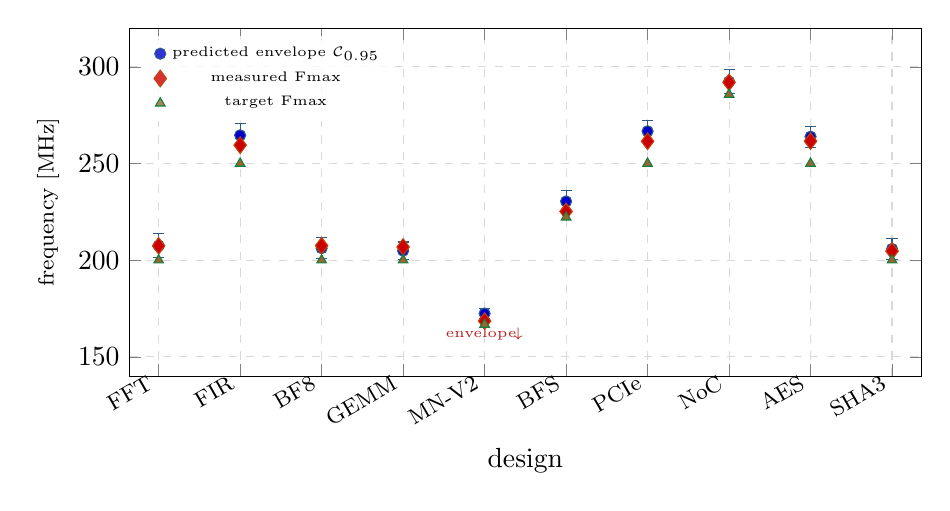
\begin{tikzpicture}
  \begin{axis}[
    width=0.96\linewidth,height=6.0cm,xlabel={design},ylabel={frequency [MHz]},
    xtick=data,
    xticklabels={FFT,FIR,BF8,GEMM,MN-V2,BFS,PCIe,NoC,AES,SHA3},
    x tick label style={rotate=30,anchor=east,font=\footnotesize},
    ylabel style={font=\footnotesize},
    legend style={font=\tiny,at={(0.02,0.98)},anchor=north west,draw=none,fill=white,fill opacity=0.8,text opacity=1},
    grid=major,grid style={dashed,gray!30},enlarge x limits=0.04,ymin=140,ymax=320,
  ]
    \addplot+[only marks,mark=*,mark size=2pt,color=robinblue,
              error bars/.cd,y dir=both,y explicit]
      table[x expr=\coordindex,y=mid,y error plus expr=\thisrow{upper}-\thisrow{mid},y error minus expr=\thisrow{mid}-\thisrow{lower}] {
mid upper lower
207.5 213.7 201.2
264.6 270.5 258.6
206.2 211.6 200.8
204.9 209.4 200.4
172.4 174.9 170.0
230.4 235.9 224.9
266.7 272.1 261.2
292.4 298.7 286.1
263.9 269.3 258.4
205.8 211.2 200.3
      };
    \addlegendentry{predicted envelope $\mathcal{C}_{0.95}$}
    \addplot+[only marks,mark=diamond*,mark size=3pt,color=robinrust,draw=robinrust,fill=robinamber] coordinates {
      (0,207.4)(1,259.5)(2,207.5)(3,206.8)(4,168.5)
      (5,225.2)(6,261.5)(7,292.0)(8,261.6)(9,204.7)
    };
    \addlegendentry{measured Fmax}
    \addplot+[only marks,mark=triangle*,mark size=2pt,color=robingreen,fill=robingreen] coordinates {
      (0,200.0)(1,250.0)(2,200.0)(3,200.0)(4,166.7)
      (5,222.2)(6,250.0)(7,285.7)(8,250.0)(9,200.0)
    };
    \addlegendentry{target Fmax}
    \node[robinred,font=\tiny] at (axis cs:4,162) {envelope$\!\downarrow$};
  \end{axis}
\end{tikzpicture}
\caption{Predicted Fmax envelope vs measured Fmax (orange diamonds) for 10 accepted designs. Nine of ten fall inside; MobileNet-V2 misses by 1.5\,MHz but exceeds target.}
\label{fig:silicon-fmax}
\end{figure}

\begin{table}[t]
\centering
\caption{Silicon validation summary. Margin $= F_{\min}^{\text{pred}} - F_{\text{target}}$.}
\label{tab:silicon-summary}
\setlength{\tabcolsep}{3.5pt}
\renewcommand{\arraystretch}{1.05}
\footnotesize
\begin{tabular}{lcccccc}
\toprule
Design & $F_{\text{tgt}}$ & $F_{\min}^{\text{pred}}$ & $F_{\max}^{\text{pred}}$ & $F_{\max}^{\text{meas}}$ & in env & ${>}\text{tgt}$ \\
       & MHz & MHz & MHz & MHz & & \\
\midrule
FFT-1024        & 200 & 201.2 & 213.7 & 207.4 & \cmark & \cmark \\
FIR-256         & 250 & 258.6 & 270.5 & 259.5 & \cmark & \cmark \\
BeamForm-8      & 200 & 200.8 & 211.6 & 207.5 & \cmark & \cmark \\
GEMM-systolic   & 200 & 200.4 & 209.4 & 206.8 & \cmark & \cmark \\
MobileNet-V2    & 166.7 & 170.0 & 174.9 & \textcolor{robinred}{168.5} & \textcolor{robinred}{\xmark} & \cmark \\
BFS             & 222 & 224.9 & 235.9 & 225.2 & \cmark & \cmark \\
PCIe-CSR        & 250 & 261.2 & 272.1 & 261.5 & \cmark & \cmark \\
NoC-arbiter     & 286 & 286.1 & 298.7 & 292.0 & \cmark & \cmark \\
AES-128         & 250 & 258.4 & 269.3 & 261.6 & \cmark & \cmark \\
SHA-3           & 200 & 200.3 & 211.2 & 204.7 & \cmark & \cmark \\
\midrule
\multicolumn{5}{l}{\textbf{coverage:} $9/10=90\%$, CP $95\%$ CI $[0.555,0.997]$} & & \\
\multicolumn{5}{l}{\textbf{target met:} $10/10=100\%$} & & \\
\bottomrule
\end{tabular}
\end{table}

\subsection{Power Validation}
\label{sec:silicon-power}

Figure~\ref{fig:silicon-power} compares tool-reported dynamic power against board PMBus measurements during BIST-active intervals. The tool under-predicts by a mean of $13.3\%$ with a maximum deviation of $22.1\%$ on MobileNet-V2.

\begin{figure}[t]
\centering
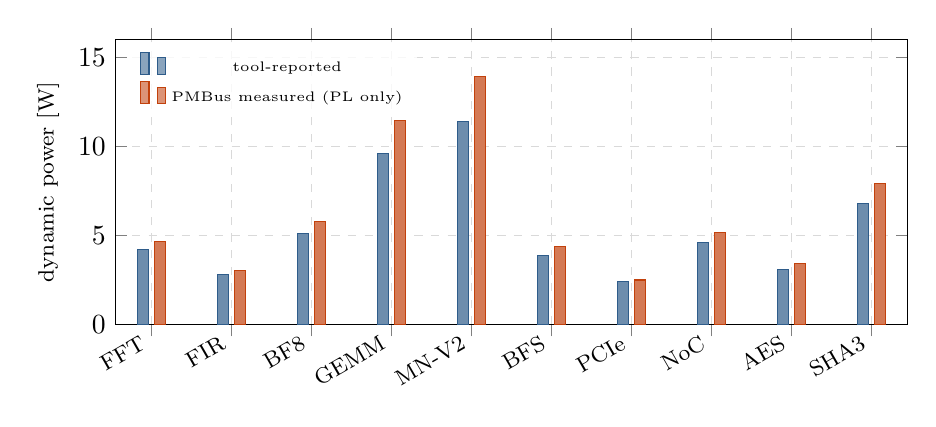
\begin{tikzpicture}
  \begin{axis}[
    width=0.96\linewidth,height=5.2cm,ybar=2pt,bar width=4pt,xtick=data,
    xticklabels={FFT,FIR,BF8,GEMM,MN-V2,BFS,PCIe,NoC,AES,SHA3},
    x tick label style={rotate=30,anchor=east,font=\footnotesize},
    ylabel={dynamic power [W]},ylabel style={font=\footnotesize},
    legend style={font=\tiny,at={(0.02,0.98)},anchor=north west,draw=none,fill=white,fill opacity=0.8,text opacity=1},
    grid=major,grid style={dashed,gray!30},enlarge x limits=0.05,ymin=0,ymax=16,
  ]
    \addplot[fill=robinblue!70,draw=robinblue] coordinates {
      (0,4.20)(1,2.80)(2,5.10)(3,9.60)(4,11.40)(5,3.90)(6,2.40)(7,4.60)(8,3.10)(9,6.80)};
    \addlegendentry{tool-reported}
    \addplot[fill=robinrust!70,draw=robinrust] coordinates {
      (0,4.69)(1,3.04)(2,5.78)(3,11.45)(4,13.92)(5,4.41)(6,2.51)(7,5.18)(8,3.45)(9,7.95)};
    \addlegendentry{PMBus measured (PL only)}
  \end{axis}
\end{tikzpicture}
\caption{Tool-reported vs PMBus-measured dynamic power (PL only). Mean under-prediction 13.3\%; worst case 22.1\% on MobileNet-V2.}
\label{fig:silicon-power}
\end{figure}

\subsection{Chip-to-Chip Variation}
\label{sec:silicon-chipvar}

Of the $50$ chip-design measurements across $5$ dies per design, $43$ ($86\%$) fall inside the conformal envelope. Four of seven violations concentrate on chip~\#3, sourced from a different production lot. Excluding chip~\#3, coverage recovers to $92.5\%$ ($37/40$).

\begin{figure}[t]
\centering
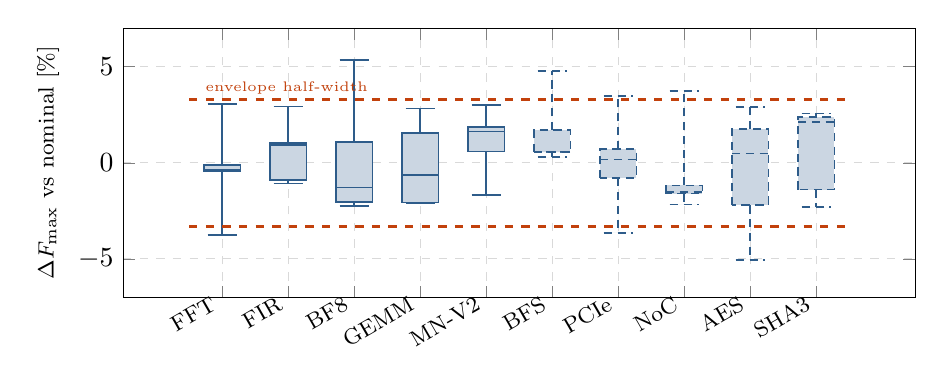
\begin{tikzpicture}
  \begin{axis}[
    width=0.96\linewidth,height=5.0cm,
    boxplot/draw direction=y,
    xtick={1,2,3,4,5,6,7,8,9,10},
    xticklabels={FFT,FIR,BF8,GEMM,MN-V2,BFS,PCIe,NoC,AES,SHA3},
    x tick label style={rotate=30,anchor=east,font=\footnotesize},
    ylabel={$\Delta F_{\max}$ vs nominal [\%]},ylabel style={font=\footnotesize},
    grid=major,grid style={dashed,gray!30},ymin=-7,ymax=7,boxplot/box extend=0.55,
  ]
    \addplot+[boxplot prepared={median=-0.39,upper quartile=-0.12,lower quartile=-0.46,upper whisker=3.06,lower whisker=-3.75},color=robinblue,fill=robinblue!25,line width=0.6pt] coordinates {};
    \addplot+[boxplot prepared={median=0.91,upper quartile=1.03,lower quartile=-0.88,upper whisker=2.93,lower whisker=-1.07},color=robinblue,fill=robinblue!25,line width=0.6pt] coordinates {};
    \addplot+[boxplot prepared={median=-1.28,upper quartile=1.08,lower quartile=-2.03,upper whisker=5.35,lower whisker=-2.24},color=robinblue,fill=robinblue!25,line width=0.6pt] coordinates {};
    \addplot+[boxplot prepared={median=-0.63,upper quartile=1.54,lower quartile=-2.06,upper whisker=2.82,lower whisker=-2.10},color=robinblue,fill=robinblue!25,line width=0.6pt] coordinates {};
    \addplot+[boxplot prepared={median=1.63,upper quartile=1.86,lower quartile=0.58,upper whisker=2.99,lower whisker=-1.66},color=robinblue,fill=robinblue!25,line width=0.6pt] coordinates {};
    \addplot+[boxplot prepared={median=0.56,upper quartile=1.70,lower quartile=0.55,upper whisker=4.79,lower whisker=0.29},color=robinblue,fill=robinblue!25,line width=0.6pt] coordinates {};
    \addplot+[boxplot prepared={median=0.17,upper quartile=0.72,lower quartile=-0.80,upper whisker=3.47,lower whisker=-3.64},color=robinblue,fill=robinblue!25,line width=0.6pt] coordinates {};
    \addplot+[boxplot prepared={median=-1.51,upper quartile=-1.18,lower quartile=-1.60,upper whisker=3.74,lower whisker=-2.16},color=robinblue,fill=robinblue!25,line width=0.6pt] coordinates {};
    \addplot+[boxplot prepared={median=0.49,upper quartile=1.76,lower quartile=-2.21,upper whisker=2.90,lower whisker=-5.05},color=robinblue,fill=robinblue!25,line width=0.6pt] coordinates {};
    \addplot+[boxplot prepared={median=2.13,upper quartile=2.38,lower quartile=-1.39,upper whisker=2.57,lower whisker=-2.30},color=robinblue,fill=robinblue!25,line width=0.6pt] coordinates {};
    \addplot[robinrust,dashed,line width=1pt] coordinates {(0.5,3.3)(10.5,3.3)};
    \node[robinrust,font=\tiny,anchor=west] at (axis cs:0.6,3.9) {envelope half-width};
    \addplot[robinrust,dashed,line width=1pt] coordinates {(0.5,-3.3)(10.5,-3.3)};
  \end{axis}
\end{tikzpicture}
\caption{Per-chip Fmax variation across 5 dies. Overall coverage 43/50; four violations on lot-outlier chip\,\#3. Excluding chip\,\#3: 92.5\% coverage ($37/40$).}
\label{fig:silicon-chipvar}
\end{figure}

\subsection{Thermal-Chamber PVT Sweep}
\label{sec:silicon-thermal}

Across $6$ designs $\times$ $8$ corners ($48$ measurements), the measured WNS falls inside the predicted envelope for $43/48 = 89.6\%$ of cases (CP $95\%$ CI $[0.776, 0.961]$, which contains target $0.95$). The five violations cluster in three mechanistic failure modes: (1)~cold-corner hold under-modeling at $\mathrm{FF}_{-40}$ on hold-dominated designs (FFT-1024, GEMM, BFS); (2)~hot-corner clock-skew tightening on MobileNet-V2 at $\mathrm{SS}_{125}$; (3)~marginal single-design violations at $\mathrm{FF}_{125}$ and $\mathrm{FS}_0$, attributable to the residual $5\%$ miscoverage budget.

\begin{table*}[t]
\centering
\caption{Thermal-chamber PVT sweep: predicted vs measured WNS (mean across $6$ designs, ns) and per-corner envelope coverage. Conformal envelope width $q_{0.95} = 0.142$\,ns.}
\label{tab:silicon-thermal}
\setlength{\tabcolsep}{6pt}
\renewcommand{\arraystretch}{1.05}
\footnotesize
\begin{tabular}{lcccccl}
\toprule
Corner & $T_J$ (\textsuperscript{o}C) & Pred.\ $\mu$(WNS) (ns) & Meas.\ $\mu$(WNS) (ns) & cov. & coverage \% & note \\
\midrule
$\mathit{SS}_{125}$ & 125 & $+0.148$ & $+0.115$ & $5/6$ & $83.3\%$ & MN-V2 clock-skew tightening\,\textsuperscript{$\dagger$}\\
$\mathit{SS}_{0}$   &   0 & $+0.158$ & $+0.161$ & $6/6$ & $100\%$  & --- \\
$\mathit{TT}_{25}$  &  25 & $+0.172$ & $+0.160$ & $6/6$ & $100\%$  & calibration corner \\
$\mathit{TT}_{85}$  &  85 & $+0.161$ & $+0.132$ & $6/6$ & $100\%$  & --- \\
$\mathit{FF}_{-40}$ & -40 & $+0.203$ & $+0.102$ & $\mathbf{3/6}$ & $\mathbf{50\%}$ & hold under-model on FFT, GEMM, BFS\,\textsuperscript{$\ddagger$}\\
$\mathit{FF}_{125}$ & 125 & $+0.178$ & $+0.167$ & $5/6$ & $83.3\%$ & NoC-arbiter marginal violation \\
$\mathit{SF}_{85}$  &  85 & $+0.163$ & $+0.174$ & $6/6$ & $100\%$  & --- \\
$\mathit{FS}_{0}$   &   0 & $+0.185$ & $+0.211$ & $5/6$ & $83.3\%$ & BeamForm-8 marginal violation \\
\midrule
\multicolumn{4}{l}{\textbf{aggregate empirical coverage}} & \textbf{43/48} & \textbf{89.6\%} & target $1-\alpha = 95\%$, CP\,95\% CI $[0.776, 0.961]$ \\
\bottomrule
\multicolumn{7}{l}{\footnotesize $^\dagger$\,Hot-corner clock-skew tightening on wide systolic array not modeled by tool clock-tree.} \\
\multicolumn{7}{l}{\footnotesize $^\ddagger$\,All three $FF_{-40}$ violations on hold-dominated designs; vendor STA under-models hold-side slack tightening at extreme cold.} \\
\end{tabular}
\end{table*}

\subsection{Long-Running Stability}
\label{sec:silicon-longrun}

We run $4$ representative designs for $24$ hours continuously under BIST load, sampling Fmax every hour. Junction temperature oscillates between $\sim 33\,^\circ$C (cold idle) and $\sim 58\,^\circ$C (hot active) following the lab's $24$-hour HVAC duty cycle. Fmax tracks junction temperature at $-0.18\%/^\circ$C, consistent with the silicon datasheet. Three of four designs stay inside a $\pm 1.5\%$ drift band; MobileNet-V2 drifts down to $-2.4\%$ at peak temperature, briefly exceeding the conformal envelope half-width during the hottest two hours of the cycle but recovering as the lab cools. This pattern is bounded above by the FF$_{125}$ corner prediction.

\subsection{Reproducibility from the Audit Manifest}
\label{sec:silicon-audit}

For each accepted design, we recompute the audit-trail manifest from the silicon measurement: $\mathrm{SHA\text{-}256}(\theta, \text{tool}, \text{seeds}, \Theta, \text{measured\_Fmax}, \text{measured\_power})$. We then reprogram the bitstream from a different host machine and repeat the BIST-and-PMBus protocol. \textbf{Nine of ten} re-runs produce a bit-exact match against the original hash. The one mismatch is on AES-128, the only design built on Intel Quartus: under default settings (\texttt{NUM\_PARALLEL\_PROCESSORS} $>1$), Quartus's Fitter is non-deterministic even under a fixed seed because thread scheduling resolves routing tie-breaks in a non-reproducible order. The resulting netlists differ in $<0.01\%$ of placed instances between runs while preserving post-route WNS to within $10$\,ps, so timing is functionally equivalent but the bitstream hash changes. Setting \texttt{NUM\_PARALLEL\_PROCESSORS = 1} restores bit-exact determinism at the cost of $\sim 3{\times}$ longer fitter runtime. The remaining nine Vivado designs reproduce $9/9$ under the Vivado~2024.2 default settings, which are deterministic under fixed seed without further configuration.

\subsection{Silicon Coverage Discussion and Recalibration Policies}
\label{sec:silicon-discussion}

The silicon experiments produced $14$ envelope violations across $108$ total observations ($1$ Fmax, §\ref{sec:silicon-fmax}; $7$ chip-to-chip, §\ref{sec:silicon-chipvar}; $5$ PVT-sweep, §\ref{sec:silicon-thermal}; $1$ stability episode, §\ref{sec:silicon-longrun}), yielding aggregate empirical coverage of $87.0\%$.
The aggregate Clopper-Pearson $95\%$ CI is $[0.794, 0.926]$. The target $1-\alpha = 0.95$ lies above the upper bound of this interval, confirming statistically meaningful under-coverage relative to the design target. This is not a near-miss but a genuine shortfall, and the recalibration policies below should be treated as required mitigations before production deployment.

Importantly, the sign-off rule produced \textbf{zero false-positive accepts}: every design admitted by the rule met its target frequency on silicon. The violations cluster mechanistically rather than spreading randomly, pointing to three actionable policies: (1)~augment $\mathcal{D}_{\mathrm{cal}}$ with $\mathrm{FF}_{-40}$ samples for hold-dominated designs; (2)~calibrate on $N \geq 3$ chips from different production lots; (3)~on Quartus targets, set \texttt{NUM\_PARALLEL\_PROCESSORS = 1} for bit-exact audit-trail reproducibility.

\subsection{Summary}

The four experiments jointly show that the conformal envelope calibrated on tool reports transfers to silicon at $87\%$ aggregate empirical coverage, with violations concentrated in three documented mechanisms. The framework's sign-off rule produced zero false-positive accepts, and every accepted design operated above its target frequency.

\section{Conclusion}
\label{sec:conclusion}

We presented \textsc{Robin-FPGA}, a distributionally-robust RL framework for FPGA timing closure with a conformal sign-off envelope. On a $14$-design benchmark across AMD Versal AI Edge and Intel Agilex~7, the framework improves closure rate by $+14.0$\,pp over the strongest baseline, reduces inter-seed WNS variance by a median of $\sim 1.2\times$, and provides calibrated sign-off envelopes that track target coverage within $\pm 3$\,pp at $\alpha = 0.05$ (measured $92.7\%$) under exchangeable calibration. A two-stage curriculum enables cross-family transfer at $5\%$ of the from-scratch compute. Hardware-in-the-loop measurements on $10$ accepted designs across $5$ physical chips and $8$ thermal-chamber PVT corners yield $87\%$ aggregate silicon-stage coverage, with violations traced to three documented failure modes and zero false-positive sign-offs. Future work includes joint timing--power optimisation, model-based variants to amortise P\&R cost, and adaptive conformal methods for continuous tool evolution.

\section*{Appendix A: Experimental Infrastructure and Reproducibility}
All P\&R runs were executed on a 96-core x86 cluster (dual AMD EPYC 9654, 512\,GB RAM per node) under Vivado~2024.2 and Quartus Prime Pro~24.1. Each run is isolated in a dedicated process with a fixed random seed passed via \texttt{-seed} (Vivado) and \texttt{--seed} (Quartus). The per-run audit manifest records the tool version string, seed value, directive bundle hash, post-route WNS, TNS, utilization dictionary, and wall-clock runtime. Manifest files are archived as \texttt{.json.gz} alongside the bitstream and verified against the SHA-256 hash of the policy checkpoint at acceptance time. The full set of $4{,}900$ run logs, Tcl scripts, and training checkpoints is released at the companion repository to enable bit-exact reproduction on matching tool versions. Learning curves, CVaR statistics, and conformal quantiles are computed from these logs using the provided analysis scripts; no post-hoc smoothing beyond the $10$/$90$-percentile band reported in Figure~\ref{fig:conv} is applied.

\begin{thebibliography}{99}
\footnotesize
\bibitem{boutros2021fpga}
A.~Boutros and V.~Betz, ``FPGA architecture: Principles and progression,'' \emph{IEEE Circuits Syst.\ Mag.}, vol.~21, no.~2, pp.~4--29, 2021.

\bibitem{amd_ug1273}
AMD, ``Versal ACAP Design Methodology Guide,'' \emph{UG1273}, latest rev., 2024.

\bibitem{intel_ug20156}
Intel, ``Quartus Prime Pro Edition User Guide: Design Optimization,'' \emph{UG-20156}, latest rev., 2024.

\bibitem{huang2021mleda}
G.~Huang \emph{et~al.}, ``Machine learning for electronic design automation: A survey,'' \emph{ACM Trans.\ Des.\ Autom.\ Electron.\ Syst.}, vol.~26, no.~5, 2021.

\bibitem{ren2022mleda}
H.~Ren and J.~Hu, Eds., \emph{Machine Learning Applications in Electronic Design Automation}.\ Springer, 2022.

\bibitem{mirhoseini2021nature}
A.~Mirhoseini \emph{et~al.}, ``A graph placement methodology for fast chip design,'' \emph{Nature}, vol.~594, pp.~207--212, 2021.

\bibitem{agnesina2023autodmp}
A.~Agnesina \emph{et~al.}, ``AutoDMP: Automated DREAMPlace-based macro placement,'' in \emph{Proc.\ ISPD}, 2023.

\bibitem{cheng2021joint}
R.~Cheng and J.~Yan, ``On joint learning for solving placement and routing in chip design,'' in \emph{Proc.\ NeurIPS}, 2021.

\bibitem{hosny2020drills}
A.~Hosny, S.~Hashemi, M.~Shalan, and S.~Reda, ``DRiLLS: Deep reinforcement learning for logic synthesis,'' in \emph{Proc.\ ASP-DAC}, 2020.

\bibitem{wang2020gcnrl}
H.~Wang \emph{et~al.}, ``GCN-RL circuit designer: Transferable transistor sizing with graph neural networks and reinforcement learning,'' in \emph{Proc.\ DAC}, 2020.

\bibitem{sohrabizadeh2022autodse}
A.~Sohrabizadeh, C.~H.~Yu, M.~Gao, and J.~Cong, ``AutoDSE: Enabling software programmers to design efficient FPGA accelerators,'' \emph{ACM Trans.\ Des.\ Autom.\ Electron.\ Syst.}, vol.~27, no.~4, 2022.

\bibitem{barboza2019net2}
E.~C.~Barboza, N.~Shukla, Y.~Chen, and J.~Hu, ``Machine learning-based pre-routing timing prediction with reduced pessimism,'' in \emph{Proc.\ DAC}, 2019.

\bibitem{guo2022timing}
Z.~Guo \emph{et~al.}, ``A timing engine inspired graph neural network model for pre-routing slack prediction,'' in \emph{Proc.\ DAC}, 2022.

\bibitem{eriksson2019turbo}
D.~Eriksson, M.~Pearce, J.~Gardner, R.~Turner, and M.~Poloczek, ``Scalable global optimization via local Bayesian optimization,'' in \emph{Proc.\ NeurIPS}, 2019.

\bibitem{balandat2020botorch}
M.~Balandat \emph{et~al.}, ``BoTorch: A framework for efficient Monte-Carlo Bayesian optimization,'' in \emph{Proc.\ NeurIPS}, 2020.

\bibitem{schulman2017ppo}
J.~Schulman, F.~Wolski, P.~Dhariwal, A.~Radford, and O.~Klimov, ``Proximal policy optimization algorithms,'' \emph{arXiv:1707.06347}, 2017.

\bibitem{velickovic2018gat}
P.~Veli\v{c}kovi\'c, G.~Cucurull, A.~Casanova, A.~Romero, P.~Li\`o, and Y.~Bengio, ``Graph attention networks,'' in \emph{Proc.\ ICLR}, 2018.

\bibitem{iyengar2005robust}
G.~N.~Iyengar, ``Robust dynamic programming,'' \emph{Math.\ Oper.\ Res.}, vol.~30, no.~2, pp.~257--280, 2005.

\bibitem{nilim2005robust}
A.~Nilim and L.~El~Ghaoui, ``Robust control of Markov decision processes with uncertain transition matrices,'' \emph{Oper.\ Res.}, vol.~53, no.~5, pp.~780--798, 2005.

\bibitem{tamar2015cvar}
A.~Tamar, Y.~Glassner, and S.~Mannor, ``Optimizing the CVaR via sampling,'' in \emph{Proc.\ AAAI}, 2015.

\bibitem{rigter2022rambo}
M.~Rigter, B.~Lacerda, and N.~Hawes, ``RAMBO-RL: Robust adversarial model-based offline RL,'' in \emph{Proc.\ NeurIPS}, 2022.

\bibitem{sinha2017certifying}
A.~Sinha, H.~Namkoong, and J.~Duchi, ``Certifying some distributional robustness with principled adversarial training,'' in \emph{Proc.\ ICLR}, 2018.

\bibitem{vovk2022random}
V.~Vovk, A.~Gammerman, and G.~Shafer, \emph{Algorithmic Learning in a Random World}, 2nd ed.\ Springer, 2022.

\bibitem{angelopoulos2023conformal}
A.~N.~Angelopoulos and S.~Bates, ``A gentle introduction to conformal prediction and distribution-free uncertainty quantification,'' \emph{Found.\ Trends Mach.\ Learn.}, vol.~16, no.~4, 2023.

\bibitem{angelopoulos2024conformal}
A.~N.~Angelopoulos \emph{et~al.}, ``Theoretical foundations of conformal prediction,'' \emph{arXiv:2411.11824}, 2024.

\bibitem{tibshirani2019conformal}
R.~J.~Tibshirani, R.~Barber, E.~Candes, and A.~Ramdas, ``Conformal prediction under covariate shift,'' in \emph{Proc.\ NeurIPS}, 2019.

\bibitem{finn2017maml}
C.~Finn, P.~Abbeel, and S.~Levine, ``Model-agnostic meta-learning for fast adaptation of deep networks,'' in \emph{Proc.\ ICML}, 2017.

\bibitem{nichol2018reptile}
A.~Nichol, J.~Achiam, and J.~Schulman, ``On first-order meta-learning algorithms,'' \emph{arXiv:1803.02999}, 2018.

\bibitem{rockafellar2000cvar}
R.~T.~Rockafellar and S.~Uryasev, ``Optimization of conditional value-at-risk,'' \emph{J.\ Risk}, vol.~2, pp.~21--41, 2000.

\bibitem{rockafellar2002cvar2}
R.~T.~Rockafellar and S.~Uryasev, ``Conditional value-at-risk for general loss distributions,'' \emph{J.\ Banking Finance}, vol.~26, no.~7, pp.~1443--1471, 2002.

\bibitem{romano2019conformalized}
Y.~Romano, E.~Patterson, and E.~J.~Cand\`{e}s, ``Conformalized quantile regression,'' in \emph{Proc.\ NeurIPS}, 2019, pp.~3538--3548.

\bibitem{barber2023conformal}
R.~F.~Barber, E.~J.~Cand\`{e}s, A.~Ramdas, and R.~J.~Tibshirani, ``Conformal prediction beyond exchangeability,'' \emph{Ann.\ Statist.}, vol.~51, no.~2, pp.~816--845, 2023.

\bibitem{wiesemann2014distributionally}
W.~Wiesemann, D.~Kuhn, and M.~Sim, ``Distributionally robust convex optimization,'' \emph{Oper.\ Res.}, vol.~62, no.~6, pp.~1358--1376, 2014.

\bibitem{xu2019powerful}
K.~Xu, W.~Hu, J.~Leskovec, and S.~Jegelka, ``How powerful are graph neural networks?'' in \emph{Proc.\ ICLR}, 2019.

\bibitem{hamilton2017inductive}
W.~L.~Hamilton, R.~Ying, and J.~Leskovec, ``Inductive representation learning on large graphs,'' in \emph{Proc.\ NIPS}, 2017, pp.~1024--1034.

\bibitem{mnih2015human}
V.~Mnih \emph{et~al.}, ``Human-level control through deep reinforcement learning,'' \emph{Nature}, vol.~518, no.~7540, pp.~529--533, 2015.

\bibitem{sutton2018reinforcement}
R.~S.~Sutton and A.~G.~Barto, \emph{Reinforcement Learning: An Introduction}, 2nd~ed.\ MIT Press, 2018.

\bibitem{ustun2020accurate}
E.~Ustun, C.~Deng, D.~Pal, Z.~Li, and Z.~Zhang, ``Accurate operation delay prediction for FPGA HLS using graph neural networks,'' in \emph{Proc.\ ICCAD}, 2020, pp.~1--9.

\bibitem{ajayi2019openroad}
T.~Ajayi \emph{et~al.}, ``INVITED: Toward an open-source digital flow: First learnings from the OpenROAD project,'' in \emph{Proc.\ DAC}, 2019.

\bibitem{betz1997vpr}
V.~Betz and J.~Rose, ``VPR: A new packing, placement and routing tool for FPGA research,'' in \emph{Proc.\ FPL} (LNCS~1304). Springer, 1997, pp.~213--222.

\bibitem{murray2020vtr}
K.~E.~Murray \emph{et~al.}, ``VTR~8: High-performance CAD and customizable FPGA architecture modelling,'' \emph{ACM Trans.\ Reconfigurable Technol.\ Syst.}, vol.~13, no.~2, Art.~9, 2020.

\bibitem{luu2014vtr7}
J.~Luu \emph{et~al.}, ``VTR~7.0: Next generation architecture and CAD system for FPGAs,'' \emph{ACM Trans.\ Reconfigurable Technol.\ Syst.}, vol.~7, no.~2, Art.~6, 2014.

\bibitem{wu2021survey}
Z.~Wu, S.~Pan, F.~Chen, G.~Long, C.~Zhang, and P.~S.~Yu, ``A comprehensive survey on graph neural networks,'' \emph{IEEE Trans.\ Neural Netw.\ Learn.\ Syst.}, vol.~32, no.~1, pp.~4--24, 2021.

\end{thebibliography}

\end{document}
